% Created 2018-04-28 Sat 02:33
% Intended LaTeX compiler: pdflatex
\documentclass[11pt]{report}
\usepackage[utf8]{inputenc}
\usepackage[T1]{fontenc}
\usepackage{graphicx}
\usepackage{grffile}
\usepackage{longtable}
\usepackage{wrapfig}
\usepackage{rotating}
\usepackage[normalem]{ulem}
\usepackage{amsmath}
\usepackage{textcomp}
\usepackage{amssymb}
\usepackage{capt-of}
\usepackage{hyperref}
\usepackage{minted}
\renewcommand\maketitle{}
\usepackage[margin=0.8in]{geometry}
\usepackage{amssymb,amsmath}
\usepackage{fancyhdr} %For headers and footers
\pagestyle{fancy} %For headers and footers
\fancyfoot[CE,CO]{}
\fancyhead[LE,LO]{}
\usepackage{lastpage} %For getting page x of y
\usepackage{float} %Allows the figures to be positioned and formatted nicely
\restylefloat{figure} %and this command
\usepackage{hyperref}
\hypersetup{urlcolor=blue}
\usepackage{titlesec}
\setcounter{secnumdepth}{4}
\usepackage{minted}
\setminted{frame=single,framesep=10pt}
\rfoot{\thepage\ of \pageref{LastPage}}
\usepackage[parfill]{parskip}
\usepackage{subfig}
\hypersetup{colorlinks=true,linkcolor=black, citecolor=black}
\usepackage{titlesec}
\usepackage{tabularx}
\usepackage{multicol}
\usepackage{array}
\usepackage[subfigure]{tocloft}
\newcolumntype{C}{ >{\centering\arraybackslash} m{10.4cm} }
\usepackage[usenames, dvipsnames]{color}
\usepackage[nocompress]{cite}
\renewcommand{\bibname}{References}
\usepackage{framed}
\usepackage{etoolbox}
\date{}
\title{\textbf{Modelling the effects of domestication in Wheat through novel computer vision techniques}}
\hypersetup{
 pdfauthor={nathan},
 pdftitle={\textbf{Modelling the effects of domestication in Wheat through novel computer vision techniques}},
 pdfkeywords={},
 pdfsubject={},
 pdfcreator={Emacs 27.0.50 (Org mode 9.1.9)},
 pdflang={English}}
\begin{document}

\newcommand{\zebra}[3]{%
    {\realnumberstyle{#3}}%
    \begingroup
    \lst@basicstyle
    \ifodd\value{lstnumber}%
        \color{#1}%
    \else
        \color{#2}%
    \fi
        \rlap{\hspace*{\lst@numbersep}%
        \color@block{\linewidth}{\ht\strutbox}{\dp\strutbox}%
        }%
    \endgroup
}

\newcommand{\listequationsname}{List of Equations}
\newlistof{myequations}{equ}{\listequationsname}
\newcommand{\myequations}[1]{%
\addcontentsline{equ}{myequations}{\protect\numberline{\theequation}#1}\par}
\setlength{\cftmyequationsnumwidth}{2.5em}% Width of equation number in List of Equations

\hyphenpenalty=10000

  \titleformat{\chapter}[display]
     {\normalfont\huge\bfseries}{\chaptertitlename\ \thechapter}{20pt}{\Huge}
  \titlespacing*{\chapter}{10pt}{10pt}{10pt}


  % Redefine the plain page style
  \fancypagestyle{plain}{%
    \fancyhf{}%
    \renewcommand{\headrulewidth}{0pt}% Line at the header invisible
    \rfoot{\thepage\ of \pageref{LastPage}}
    \fancyfoot[CE,CO]{}
  }

  % \patchcmd{\chapter}{\thispagestyle{fancy}}{\thispagestyle{fancy}}{}{}


  \thispagestyle{empty}
  \renewcommand{\headrulewidth}{0pt}
  \begin{center}
    \fontsize{10}{12}
    \selectfont

    \textbf{\huge Modelling the effects of domestication in Wheat through novel computer vision techniques}

    \vspace{0.3in}

    \begin{tabular}[t]{ll}
      Author: & Mr. Nathan Hughes (nah26@aber.ac.uk) \\
      Supervisor: & Dr. Wayne Aubrey (waa2@aber.ac.uk) \\
      Degree Scheme &  G401 \hspace*{0.05in}(Computer Science)\\
      \\
      \\
      Date: & \today \\
      Revision: & 0.1\\
      Status: & Draft\\
      \\
    \end{tabular}
    \\
    \vspace{0.1in}
    This report was submitted as partial fulfilment \\of a BSc degree in Computer Science (G401)
  \end{center}
  \clearpage
  \renewcommand{\headrulewidth}{1pt}

  \thispagestyle{plain}

  \begin{center}
    {\LARGE\bf Declaration of originality}
  \end{center}

  I confirm that:

  \begin{itemize}
  \item{This submission is my own work, except where
      clearly indicated.}

  \item{I understand that there are severe penalties for Unacceptable Academic Practice, which can lead to loss of marks or even the withholding of a degree.}

  \item{I have read the regulations on Unacceptable Academic Practice from the University's Academic Quality and Records Office (AQRO) and the relevant sections of the current Student Handbook of the Department of Computer Science.}

  \item{In submitting this work I understand and agree to abide by the University's regulations governing these issues.}
  \end{itemize}

  \vspace{2em}
  Name ............................................................  \\

  \vspace{1em}
  Date ............................................................ \\

  \vspace{1em}
  \begin{center}
    {\LARGE\bf Consent to share this work}
  \end{center}

  By including my name below, I hereby agree to this dissertation being made available to other students and academic staff of the Aberystwyth Computer Science Department.

  \vspace{2em}
  Name ............................................................  \\

  \vspace{1em}
  Date ............................................................ \\

  \clearpage

  \thispagestyle{plain}

  \begin{center}
    {\LARGE\bf Acknowledgements}
  \end{center}

\vspace{3cm}

This work is a product of all the things Aberystwyth University has taught me, unfortunately
there is not enough space here for everyone who should be thanked and acknowledged.

\vspace{1cm}

However, in relation to this project it would be a great crime to not thank my project supervisor Dr. Wayne Aubrey for his help and guidance;
Professor. John Doonan, who provided the project and trusted me with it;
Dr. Candida Nibau who taught me practically everything I know about biology; Dr. Kevin Williams for allowing all my questions about maths and statistics;

\vspace{1cm}

My headphones, my books and all the art that kept me sane. Without J.K. Rowling, Arthur Conan-Doyle, Ben Howard and Bob Dylan
 my motivation would have dried up long ago.

\vspace{1cm}

Finally, and most importantly, my mother Barbara Hughes. Who believed in me, always.



  \clearpage
  \tableofcontents
  \clearpage
  \listoftables
  \clearpage
  \listoffigures
  \clearpage
  \listofmyequations
  \clearpage
  \listoflistings
  \clearpage

\chapter{Introduction, Analysis and Objectives}
\label{sec:org4b0a4eb}

This project aims to answer a biological research question through the use of computer science, whilst also creating a software suite which will enable further studies to be carried out with ease.

Primarily the focus has been on the data science elements of my degree, creating, cleaning and discerning meaning in it.

Using a population of genetically diverse wheat, several hypothesis and questions are explored in the hopes of contributing to the scientific understanding of plant domestication. A mixture of image analysis through three-dimensional micro-computed tomography and computational analysis are used to provide these much needed solutions.


Additionally, as this is very much multi-disciplinary research, specific terms and definitions have been outlined in the glossary (table:\ref{tab:org48f7e61}).

\section{Background}
\label{sec:org7f2ed58}

Western society and agriculture has been dominated by the ability to create successful crops for the past 10,000 years \cite{Ozkan2002}. Of these crops wheat is considered to be one of the most vital and is estimated to contribute to 20\% of the total calories and proteins consumed worldwide, and accounts for roughly 53\% of total harvested area (in China and Central Asia) \cite{Shiferaw2013}.

During domestication, the main traits selected for breeding were most likely plant height and yield. This meant that important non-expressed traits such as disease resistance and drought tolerance were often neglected and lost overtime.

Whilst the choices made for selective breeding were successful, effects are now being felt as it is estimated that as much as a 5\% dip is observed yearly for  wheat production \cite{Shiferaw2013}. This decrease in efficiency is attributed to climate change bringing in more hostile conditions, which these elite and  domesticated genotypes are unprepared for.

Furthermore, with increasing population and less arable land there is an even greater pressure for the optimisation of grain and spike characteristics. With studies showing that spikelet, the collective for seeds sharing the same node on a spike, count can be controlled by specific and sometimes recessive genes \cite{Finnegan2018}, which could drastically enhance overall yield, and a general public distrust towards genetically modification \cite{Aleksejeva2014,Twardowski2015,Lynas} the reliance on breeding programs for optimisation is further stressed.

Modern breeding programs have had some success in selecting primitive undomesticated genotypes and using them to breed back in useful alleles which would have been lost during domestication \cite{Charmet2011}.

As such, there are questions still left open about how best to make selections for crop breeding. There is also a lack of formalised modelling of information which could be of use in these areas of research.

\section{Biological Question and Materials}
\label{sec:org2b0a5da}

The driving question for this research asks "Can \textmu{}-Computed Tomography data be used to model domestication in wheat?". Using an already grown and harvested range of genetically diverse wheat this project has generated a collection of 3D images, processed these images into raw phenotypic data and produced biologically significant information.

Here, ploidy has been used as a distinguishable and important attribute of the study. Ploidy refers to the number of sets of chromosomes that an organism has, usually this is denoted by an N.

The genotypes used in this study are listed here, denoted by "\emph{X} N" where \emph{X} indicates the ploidy. 2N - Diploid; 4N - Tetraploid; 6N - Hexaploid. A \emph{W} indicates wild genotypes, \emph{D} domesticated ones.

\begin{multicols}{3}

  \begin{itemize}
  \item{\textit{T. boeoticum} (2N|W)}
  \item{\textit{T. monococcum} (2N|D)}
  \item{\textit{A. Tauschii} (2N|D)}
  \end{itemize}

  \columnbreak

  \begin{itemize}
  \item{\textit{T. durum} (4N|D)}
  \item{\textit{T. dicoccum} (4N|D)}
  \item{\textit{T. dicoccoides} (4N|W)}
  \item{\textit{T. ispahanicum}(4N|D)}
  \item{\textit{T. timopheevii} (4N|D)}
  \end{itemize}

  \columnbreak

  \begin{itemize}
  \item{\textit{T. spelta} (6N|D)}
  \item{\textit{T. aestivum} (6N|D)}
  \item{\textit{T. compactum} (6N|D)}
  \end{itemize}

\end{multicols}
Full species names are found in table:\ref{tab:orge0a0129}.

\subsection{Why use \textmu{}-CT image analysis?}
\label{sec:org4d67591}
In the past, science has been greatly limited by the amount of data which could be processed in an experiment. In the last few decades the inclusion of computer science has reduced this bottleneck. Now, the challenge for many fields of research is producing more data and this is often cited as the new limiting factor in creating robust studies \cite{Furbank2011}.

Many experiments aim to meet the demand for data by using high-throughput automated imaging systems \cite{Naumann2007,Prasanna2013,Humplik2015}. These systems have, in the last decade, become a standard and accepted tool for data generation in plant phenotype studies. However, they will only produce 2-dimensional data on a per-plant basis. Image processing research has had success in modifying these automated systems in order to produce a pseudo 3-dimensional structure using stero-imaging \cite{Roussel2016}. Even so, these techniques require destructive harvesting of plant materials and do not provide information of internal structure.

For decades medical research has found success with X-Ray imaging technology \cite{Wang2008}. From this, plant science has been able to benefit from the wealth of prior knowledge and more and more studies are being augmented with the use of X-Ray/\textmu{}-CT imaging \cite{Jhala2015,Tracy2012,Metzner2015,Hughes2017,Staedler2013}.

In this study, \textmu{}-CT has enabled the study of individual seeds of wheat, which is the product that plant breeders, commercial growers and farmers are truly interested in. Other imaging techniques could not provide as much detail, whilst retaining developmental and positional information, or in such a high throughput or quality/resolution.

\subsection{Extracted Data}
\label{sec:org18589be}

These samples come from over 70 plants and provided in excess of 2000 seeds. These data form the basis for this research and testing of the software libraries created. The traits recorded are labelled in figure:\ref{fig:orgb543efe} and are as follows:

\begin{multicols}{2}

  \begin{itemize}
  \item Length
  \item Width
  \item Depth

  \end{itemize}

  \columnbreak

  \begin{itemize}
  \item Volume
  \item Surface Area
  \item Crease Depth / Volume
  \end{itemize}
\end{multicols}


\begin{figure}[htbp]
\centering
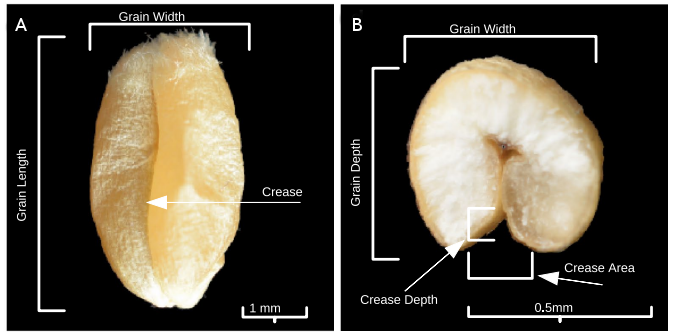
\includegraphics[width=17cm]{./images/seeds.png}
\caption{\label{fig:orgb543efe}
Wheat grain labelled (\emph{left}), wheat grain cut in half horizontally (\emph{right}), adapted from Hughes et al. \cite{Hughes2017}}
\end{figure}

\section{Significance to Current Research}
\label{sec:org58d3978}
The biological interest in this area has been expressed in several areas of research \cite{Leigh2013}, it is proposed that the key to unlocking diversity in the wheat genus lies in these ancestor, undomesticated species \cite{Cockram2007}.

This research has the potential to be useful in several areas including: crop breeding; disease resistance; environmental stress. Each of these areas depend on making informed decisions in order to direct experiments. By producing information at an individual seed level, this study has been able to provide data that can offer suggestions of grain potential and the developmental behaviour/effects of polyloidization.

Often, the most sought after traits are centred around thousand-grain-weight (TGW) as well as standard deviation of seed shapes. During harvesting, filters are used to only allow ideal shaped seeds through. This means that, potentially, despite a breed of wheat providing a high average volume of seed in reality much of it may go to waste if the shapes are not uniform. This research aims to alleviate this problem and provides low level information which is sorely required.

The individual images in figure:\ref{fig:org36de1ea} show, at a glance, the diversity and also the difference in the wild and cultivated (domesticated)
species. This work allows for these differences to be quantified and evaluated into useful metrics for answering research based questions.

By better understanding the morphometric deviations in wheat species, more informed choices can be made when it comes to breeding wheat for the future and to fulfil ever-changing requirements.

\clearpage

\begin{figure}[htbp]
\centering
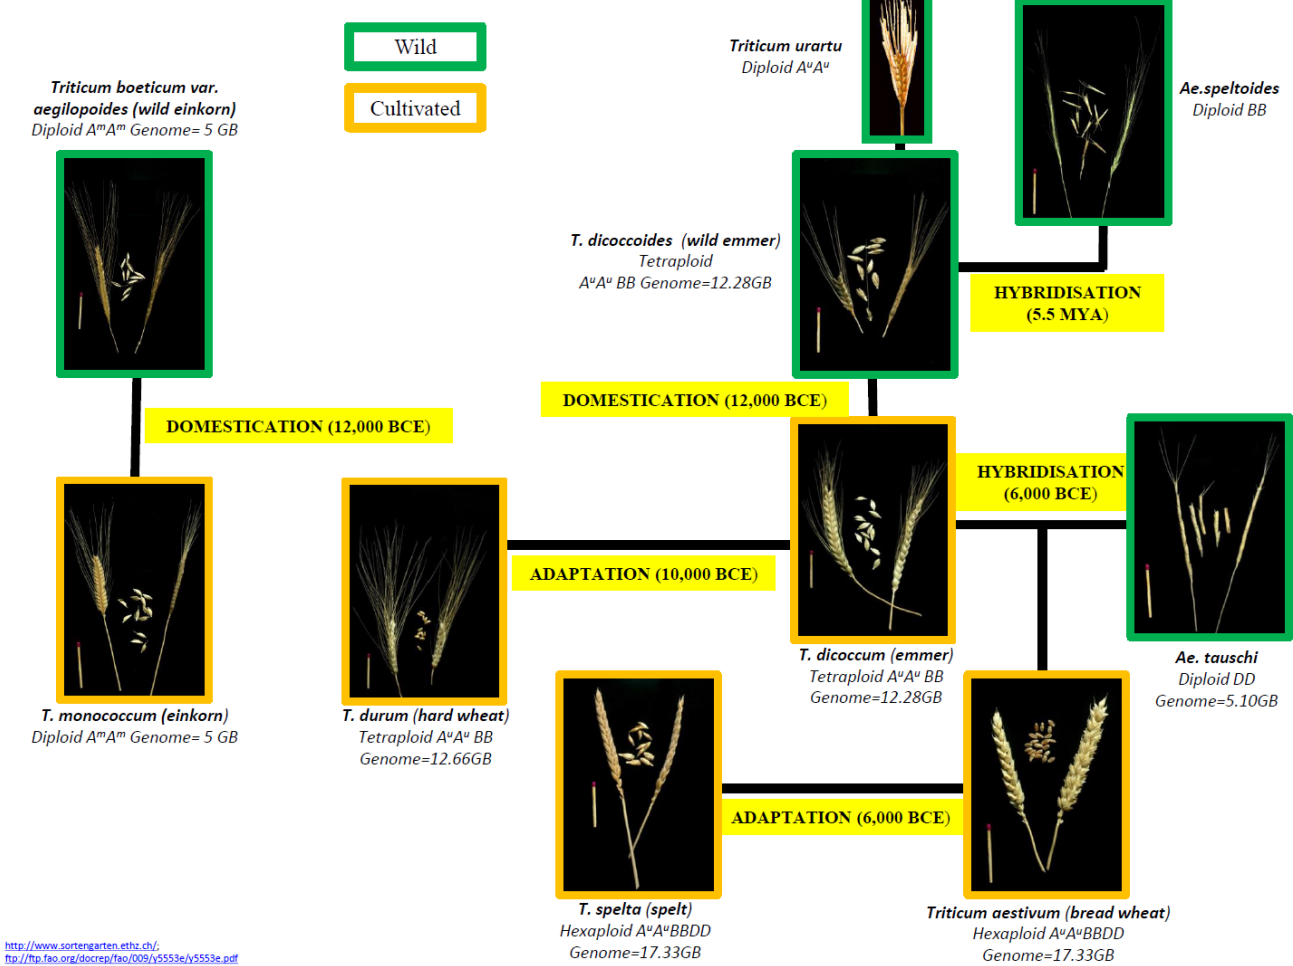
\includegraphics[width=17cm]{./images/philotree.png}
\caption{\label{fig:org36de1ea}
Phylogeny of wheat genotypes (Provided by Dr. Hugo Oliveira)}
\end{figure}

\section{Aims and Objectives}
\label{sec:orga091535}

The overarching aim of this project has been to create several pieces of software which aid in answering the biologically significant questions outlined. As well as to prove/disprove the hypothesis stated below.

The software created is robust in order to duplicate results and is flexible as to allow for further studies to be carried out and to use the same method.

Novel additions have been made to existing image analysis libraries in order to make them more flexible for this project. Figure:\ref{fig:org56794b6} illustrates the range of diversity

Furthermore, the library written allows for easy data organisation and automation of otherwise difficult tasks such as concatenating data from multiple sources and graphing of information. Full documentation and integrated testing allows for a suite of tools which can be built upon in future and reduce the amount of effort required for similar studies to be carried out and analysed.

\section{Hypothesis}
\label{sec:orga0637ed}
To provide a full spectrum of analysis the null-hypothesis of this work is presented as investigating if there are morphometric differences in the seeds of several wheat varieties outlined in figure:\ref{fig:org36de1ea}.

The comparison pairs are as follows (where W indicates wild genotypes and D domesticated.):

\begin{enumerate}
\item \emph{T. monococcum} (2N|D) and \emph{T. beoticum} (2N|W)
\item \emph{T. dicoccum} (4N|D) and \emph{T. dicoccoides} (4N|W)
\item \emph{T. spelta} (6N|D) and \emph{T. aestivum} (6N|D)
\item \emph{T. dicoccum} (4N|D) and \emph{T. durum} (4N|D)
\item \emph{T. beoticum} (2N|W) and \emph{T. dicoccoides} (4N|W)
\item \emph{T. dicoccum} (4N|D) and /T. aestivum (6N|D)
\item \emph{T. durum} (4N|D) and /T. aestivum (6N|D)
\end{enumerate}

These comparison groups where chosen, with help from researchers at the National Plant Phenomics Centre and the University of Manchester, based on their ploidy and also on their domestication grouping. This maximises the potential of this research by isolating features and attributes of wheat based on domestication status.
\begin{figure}[htbp]
\centering
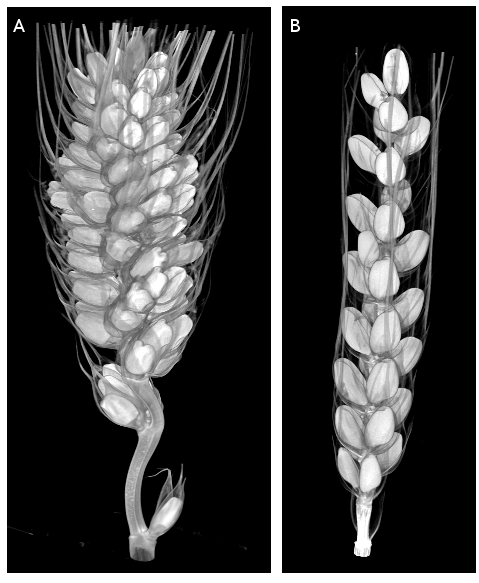
\includegraphics[width=10cm]{./images/spikes.png}
\caption{\label{fig:org56794b6}
Scans of wheat, showing diversity in Population, Compactum (6N) left, Durum right (4N)}
\end{figure}

\section{Challenges Overview}
\label{sec:org1f548fa}

The challenges which this project tackles come in two flavours: Computational and Biological. As such keen awareness of these is needed to appreciate the novelty of this work.

\subsection{Biological Challenges}
\label{sec:orgd9a20fd}
Previous studies have been able to demonstrate that variation in wheat grain morphology can be partially explained, in 2010 Gegas et al. demonstrated this through a 99.4\% 2 component PCA \cite{Gegas2010}. However there is much left to do in terms of formal classifications and descriptions of these differences. This project deals with this problem through computational analysis.

Two effects run parallel in this study, both of these need to be accounted for in the analysis, and questions need asked in a manner to extract each effect independently:

\begin{enumerate}
\item The effects of polyploidization in wheat.
\item The effects of domestication in wheat.
\end{enumerate}

Both of these effects will need to be taken into consideration so as not to misidentify results, and falsely attribute effect.

\subsection{Computational Challenges}
\label{sec:orgafe4848}
Using \textmu{}-CT data in plant sciences is becoming more and more common \cite{Tracy2017,Jhala2015,Hughes2017,Metzner2015} and whilst a lot of studies focus on the traits of grains specifically no formal model has been created, and no accepted data format. This is a data engineering problem and the methods described in this project address this.

Further to data organisation, proposals are made for the statistical analysis which should be used. This allows for studies to become more robust and repeatable, thus strengthening the studies overall and giving more confidence to results.

The biological material used in this research is much more diverse a population than has been previously studied with \textmu{}-CT image analysis. This requires current computer vision methods to be adapted in order to analyse this added diversity.

\section{Deliverables}
\label{sec:org21a0cf8}

This project provides three final deliveribles:

\begin{enumerate}
\item A flexible software suite written in \emph{Python} that provides a standardised method for analysing and interpreting \textmu{}-CT data output.
\item A Graphical User Interface (GUI) which offers a point and click method for data gathering, graphing and manipulating \textmu{}-CT data, using the library from deliverable 1 as a backend.
\item Answers to the proposed questions (hypotheses), provided in the \emph{Results} and \emph{Discussion} sections of this report.
\end{enumerate}

\chapter{Software Design, Implementation and Testing}
\label{sec:orgdc6fc3f}
This chapter outlines choices and methodologies employed in the software engineering aspect of this project, as well as highlighting the key functional requirements and implementation decisions.

\section{Functional Requirements}
\label{sec:org450e8cb}
Requirements for this project are split between software requirements for both the CT Analysing Library and the CT GUI Application and the research requirements (i.e. the answers to the proposed hypothesis). Here the requirements for the software are discussed:
\subsection{Requirements for CT Analysing Library}
\label{sec:orga3fbd63}

These are the functional requirements for the Python library produced:

\begin{multicols}{2}

  \begin{enumerate}
  \setcounter{enumi}{-1}
  \item Provide an OOP means to deal with data
  \item Make gathering of data simplified
  \item Handle Saving of data in a usable format
  \item Easily enable data transformations
  \item Perform hypothesis testing
  \end{enumerate}

  \columnbreak

  \begin{enumerate}
  \setcounter{enumi}{4}
  \item Process rejoining of split scans
  \item Handle Removing of erroneous data
  \item Enable matching data to external information
  \item Auto plot data (boxplots, histograms etc.)
  \item Allow easy filtering of data
  \end{enumerate}

  \columnbreak

\end{multicols}

\subsection{Requirements for CT GUI Application}
\label{sec:orgabe6075}


\begin{multicols}{2}

  \begin{enumerate}
  \setcounter{enumi}{9}
  \item Provide a intuitive user interface for working with CT data
  \item Allow a interaction with data without the need for programming
  \item Implement the Matplotlib plotting utility
  \item Easily join experiment data with CT data
  \item Use an MVC model
  \end{enumerate}

  \columnbreak

  \begin{enumerate}
  \setcounter{enumi}{14}
  \item Implement the CT Analysis Library
  \item Display data visually
  \item Dynamically create graphs
  \item Provide hypothesis testing
  \end{enumerate}

  \columnbreak

\end{multicols}

\section{Software Development Methodology}
\label{sec:orgc4043cb}
This project made use of formal design methods and strict organisation whilst being flexible to change. Overall the design took a hybridised form in order to best suit the scientific environment which this domain specific software is built for.

Data analysis drove the direction of the project, as a result an agile methodology was adopted.
Weekly sprints were implemented as a list of "todo's", these were written on a Monday morning based on the previous week's list.

Critical self-evaluation was performed by means of a "one-man SCRUM" meeting, this is a technique which requires self-discipline in order to accurately find faults and areas for improvement \cite{Andrews}.

Further to this, regular meetings with research staff, at the National Plant Phenomics Centre,  allowed for a developer-client relationship which SCRUM defines as being key. During these meetings details of the research was discussed and ideas given as to how future experiments could proceed. This allowed for critical decisions to be made regarding software design and overall structure.
\section{Sprint Timeline}
\label{sec:org97b53e3}
The implementation of this work was done following agile sprint planning, treating each week as a encapsulated working frame, for each of these a detailed organisational programme was created, discussed with supervisors and then used to formulate plans of action for following up on.

A full account of the sprints, which are in part running documentation for this project, are available in appendix:\ref{org8882545}.

\section{Language Choices}
\label{sec:org15b2a17}
Both the CT Analysing Library and the CT Analysing GUI are implemented using the Python programming language, it has been developed and tested in versions 3.5 and 3.6 (Python 2 is not supported at all by this project, there is an ongoing effort to move forward in scientific computing, away from Python 2.X  \cite{Ozgur2016}).

In scientific programming three of the most commonly used languages are Python, R and MATLAB \cite{Ozgur2016}.

These three languages are able to provide all the features which this project requires. However Python was chosen for several reasons.

MATLAB could not be used as a potential language due to it being pay to use software, as this project aims to be accessible, the cost of software would greatly reduce the scope of access.

R is a valid candidate, it provides all of the statistical capabilities required by the project, it also provides packages for creating GUI based applications, it is fast and it is widely used in scientific computing and data science.

The main deciding factor is Python's wealth of resources, adoption rate and the developer of this project being vastly more experienced with Python's ecosystem than R's.

\section{Designing Process}
\label{sec:orgdb0186b}
Through meetings and emails, the agile principles of communication over comprehensive documentation was used. Where conversations were decidedly much more beneficial than complex planing prior to developing a product.

Graphical elements, such as the graphing functionality of the CT Analysing Library and the CT GUI Application were sketched using wire-frames whilst in meetings where the potential users (clients) could provide their ideas.

In figure:\ref{fig:orgb3ae0e8} an example of the wire-frames created during meetings is show (A), next to it is displayed the final look of the loading window (B).
\begin{figure}[htbp]
\centering
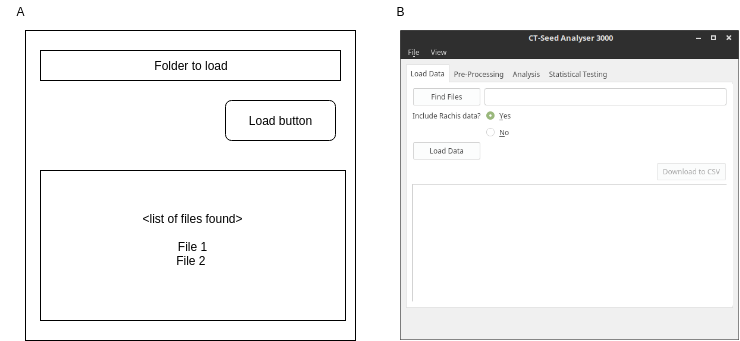
\includegraphics[width=16cm]{./images/wireframe1.png}
\caption{\label{fig:orgb3ae0e8}
Wire-frame (A) of the GUI loading data window (B)}
\end{figure}

Similarly, figure:\ref{fig:orgea83e71} provides the initial wire-frame (A) of how the analysis window could have looked and what kind of GUI elements would be required, again, next to it is the final analysis window (B)
\begin{figure}[htbp]
\centering
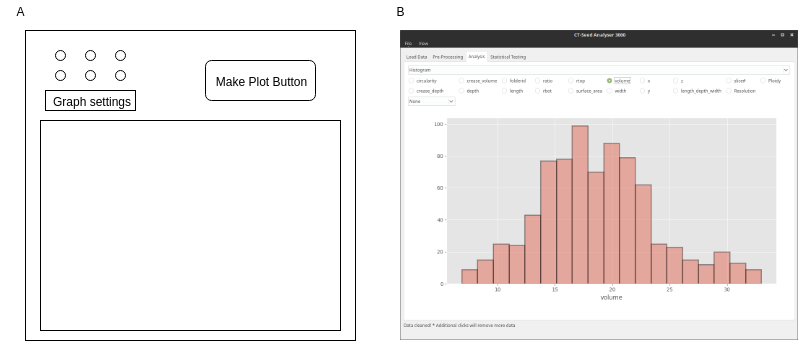
\includegraphics[width=16cm]{./images/wireframe2.png}
\caption{\label{fig:orgea83e71}
Wire-frame (A) of the GUI analysis window (B)}
\end{figure}
\section{Documentation}
\label{sec:org608c0ab}
Whilst an agile approach was used, some documentation was created for use with the CT Analysing Library.

The provided CT Analysing Library comes with "human-readable" format. Where as most documentation generators (Doxygen, Pydocs, Javadocs etc.) implement very well structured and comprehensive documentation, the output is generally not very friendly and easy to read. Particularly for non-career-programmers. A core feature of these provided software implementations are that they are well suited for a biologist, researcher or statistician to use.

This documentation generator was purpose created, implemented in LISP and provided in listing:\ref{orgaf430bd}.

Beyond this, inline commenting is provided for supplied software. Keeping in line with the agile development ethos the software is self-documented and self-evident. A brief example of this is shown in listing:\ref{orgeb46770}

Documentation for the CT GUI application is provided as a visual user guide, and provides sample data for the user to test with.
\section{Software Library Choices}
\label{sec:org256eeae}
The software libraries used for this project focus around data manipulation. Where possible, only core libraries of the Python language were used and only well supported, established and documented libraries were chosen. Software support is a major requirement for reproducible results.

All software packages used in the Analysing Library are required by the CT Analysing GUI as the Library is a dependency of it. The GUI has a single separate requirement \emph{PyQT5}.
Table:\ref{tab:org8925f5a} contains a full listing of all software used and required by this project.
\subsection{Numpy}
\label{sec:orgb9b1c6c}
The Numpy library is one of the most commonly used additions to the Python ecosystem, it is fundamental to many data science projects. Here it is used to handle data lists, arrays and structures. The data model used in this project is able to be optimised through Numpy and allows results to be calculated in seconds.
\subsection{Matplotlib/Seaborn}
\label{sec:org8c6d02b}
Matplotlib acts as the plotting backend for the project. The Seaborn package acts as a porcelain for matplotlib and makes graph creation and decoration much easier.
\subsection{SciPy}
\label{sec:orgee44eb3}
Data transforms such as Box Cox and PCA are dependant on the functions of the Scipy library. Alternatives are available, however this is the most well established and often used library for these functions. SciPy provides many of the required functions in a single package and helps reduce further software dependencies.
\subsection{Pandas}
\label{sec:org8dbfe52}
Pandas is used to read the CSV files which the raw data is stored in. This library converts and stores data in dataframes which are used throughout this project to manipulate data. Dataframes are used as the core of \emph{CTData} objects in the analysis library.
\subsection{Xlrd}
\label{sec:org527081c}
This extension library is required in order to read Microsoft encoded files. Extra experiment information can be provided with the "xlsx" extension.
\subsection{Statsmodels}
\label{sec:org64dfd64}
The backbone of the data analysis model is handled by this library, it also provides an implementation of the Markov chain Monte Carlo system used to generate random samples from the model population.
\subsection{PyQT5}
\label{sec:org67ff57f}
There were many options for creating a user interface in Python, the language provides its own core library via the \emph{TKinter} module. However PyQT is a port of the QT framework, one of the most widely used libraries for GUIs in software development. It is cross platform, robust and has excellent documentation and user-guides.

\section{Version control}
\label{sec:org2784320}
This project has used Git version 2.7.4 throughout. The structure of the project has been as submodules of a larger project.

By using submodules the CT Grain Analysing Library could be kept in sync with the GUI aspect of the project.

Additionally, \emph{setup.py} has been used to provide installation of the library, the code for this can be seen in listing:\ref{org39ea4a7}. Using \emph{setup.py} provides a quick and easy way for any user to install the software, along with any dependencies.

\subsubsection{Issue Tracking}
\label{sec:org32656d2}
Issues were tracked during the project, both in personal notes and in the Git interface as illustrated in figure:\ref{fig:orgba1d68c}
\begin{figure}[htbp]
\centering

\includegraphics[width=10cm]{./images/github.png}
\caption{\label{fig:orgba1d68c}
Github Issue Tracking}
\end{figure}

\section{Implementation Methodology}
\label{sec:org1ac5f39}
Strict software engineering principles were applied during creation of this project. The use of standards, design patterns and code-linters have been used throughout to minimise the possibility of errors and to create wholly extendable software. These devices enable understandable and self-documented code allowing future users to quickly start using the provided packages.
\subsection{Standards}
\label{sec:org994ab39}
The main standard adhered to for software provided by this project is the PEP8 style guide \cite{VanRossum}. The principle behind this coding style, as stated by Guido van Rossum, is "Code is read much more often than it is written". This makes this styling guide perfect for the chosen agile methodology of self-evident documentation in the software.

In addition to PEP8, a Python code linter Flake8 has been used to prevent "code smells", bad formatting, incorrect white space usage etc.

\subsection{CT Analysing Library Design Pattern}
\label{sec:org532219c}
The CT Analysing Library uses a Singleton style design pattern. A single data object is created from a \emph{CTData} class.

A very functional paradigm is used by this library. By applying mapping and filter style functions data elements can be passed to the supporting modules: \emph{data\_transforms.py}; \emph{graphing.py}, \emph{statistical\_tests.py}. These modules enable scientific functions to be applied to the \emph{CTData} object. A UML style class diagram is shown in figure:\ref{fig:org9fd874d}, here the interactions of the classes can be seen, as well as their internal functions.

\begin{figure}[htbp]
\centering
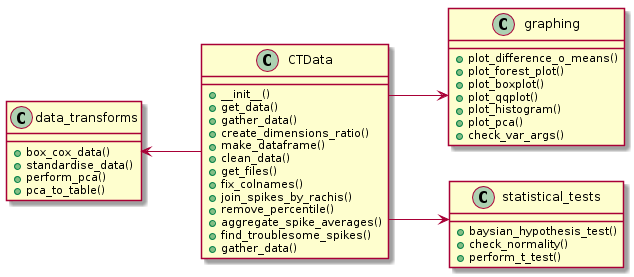
\includegraphics[width=12cm]{./images/ctdata.png}
\caption{\label{fig:org9fd874d}
CT Analysing Library UML}
\end{figure}

\subsection{CT GUI Application Design Pattern}
\label{sec:orga535361}
The Model-View-Controller (MVC) design pattern is one of the most commonly structures for creating user interfaces. It allows for the user's view/interface code to be separated from the model, the code which changes the data. The model and the view communicate and update each other via the controller element of the design.

The QT framework provides "connectors" which act as triggers/activations for functions, these are set off by the user providing either keyboard or mouse based input.

\begin{figure}[htbp]
\centering
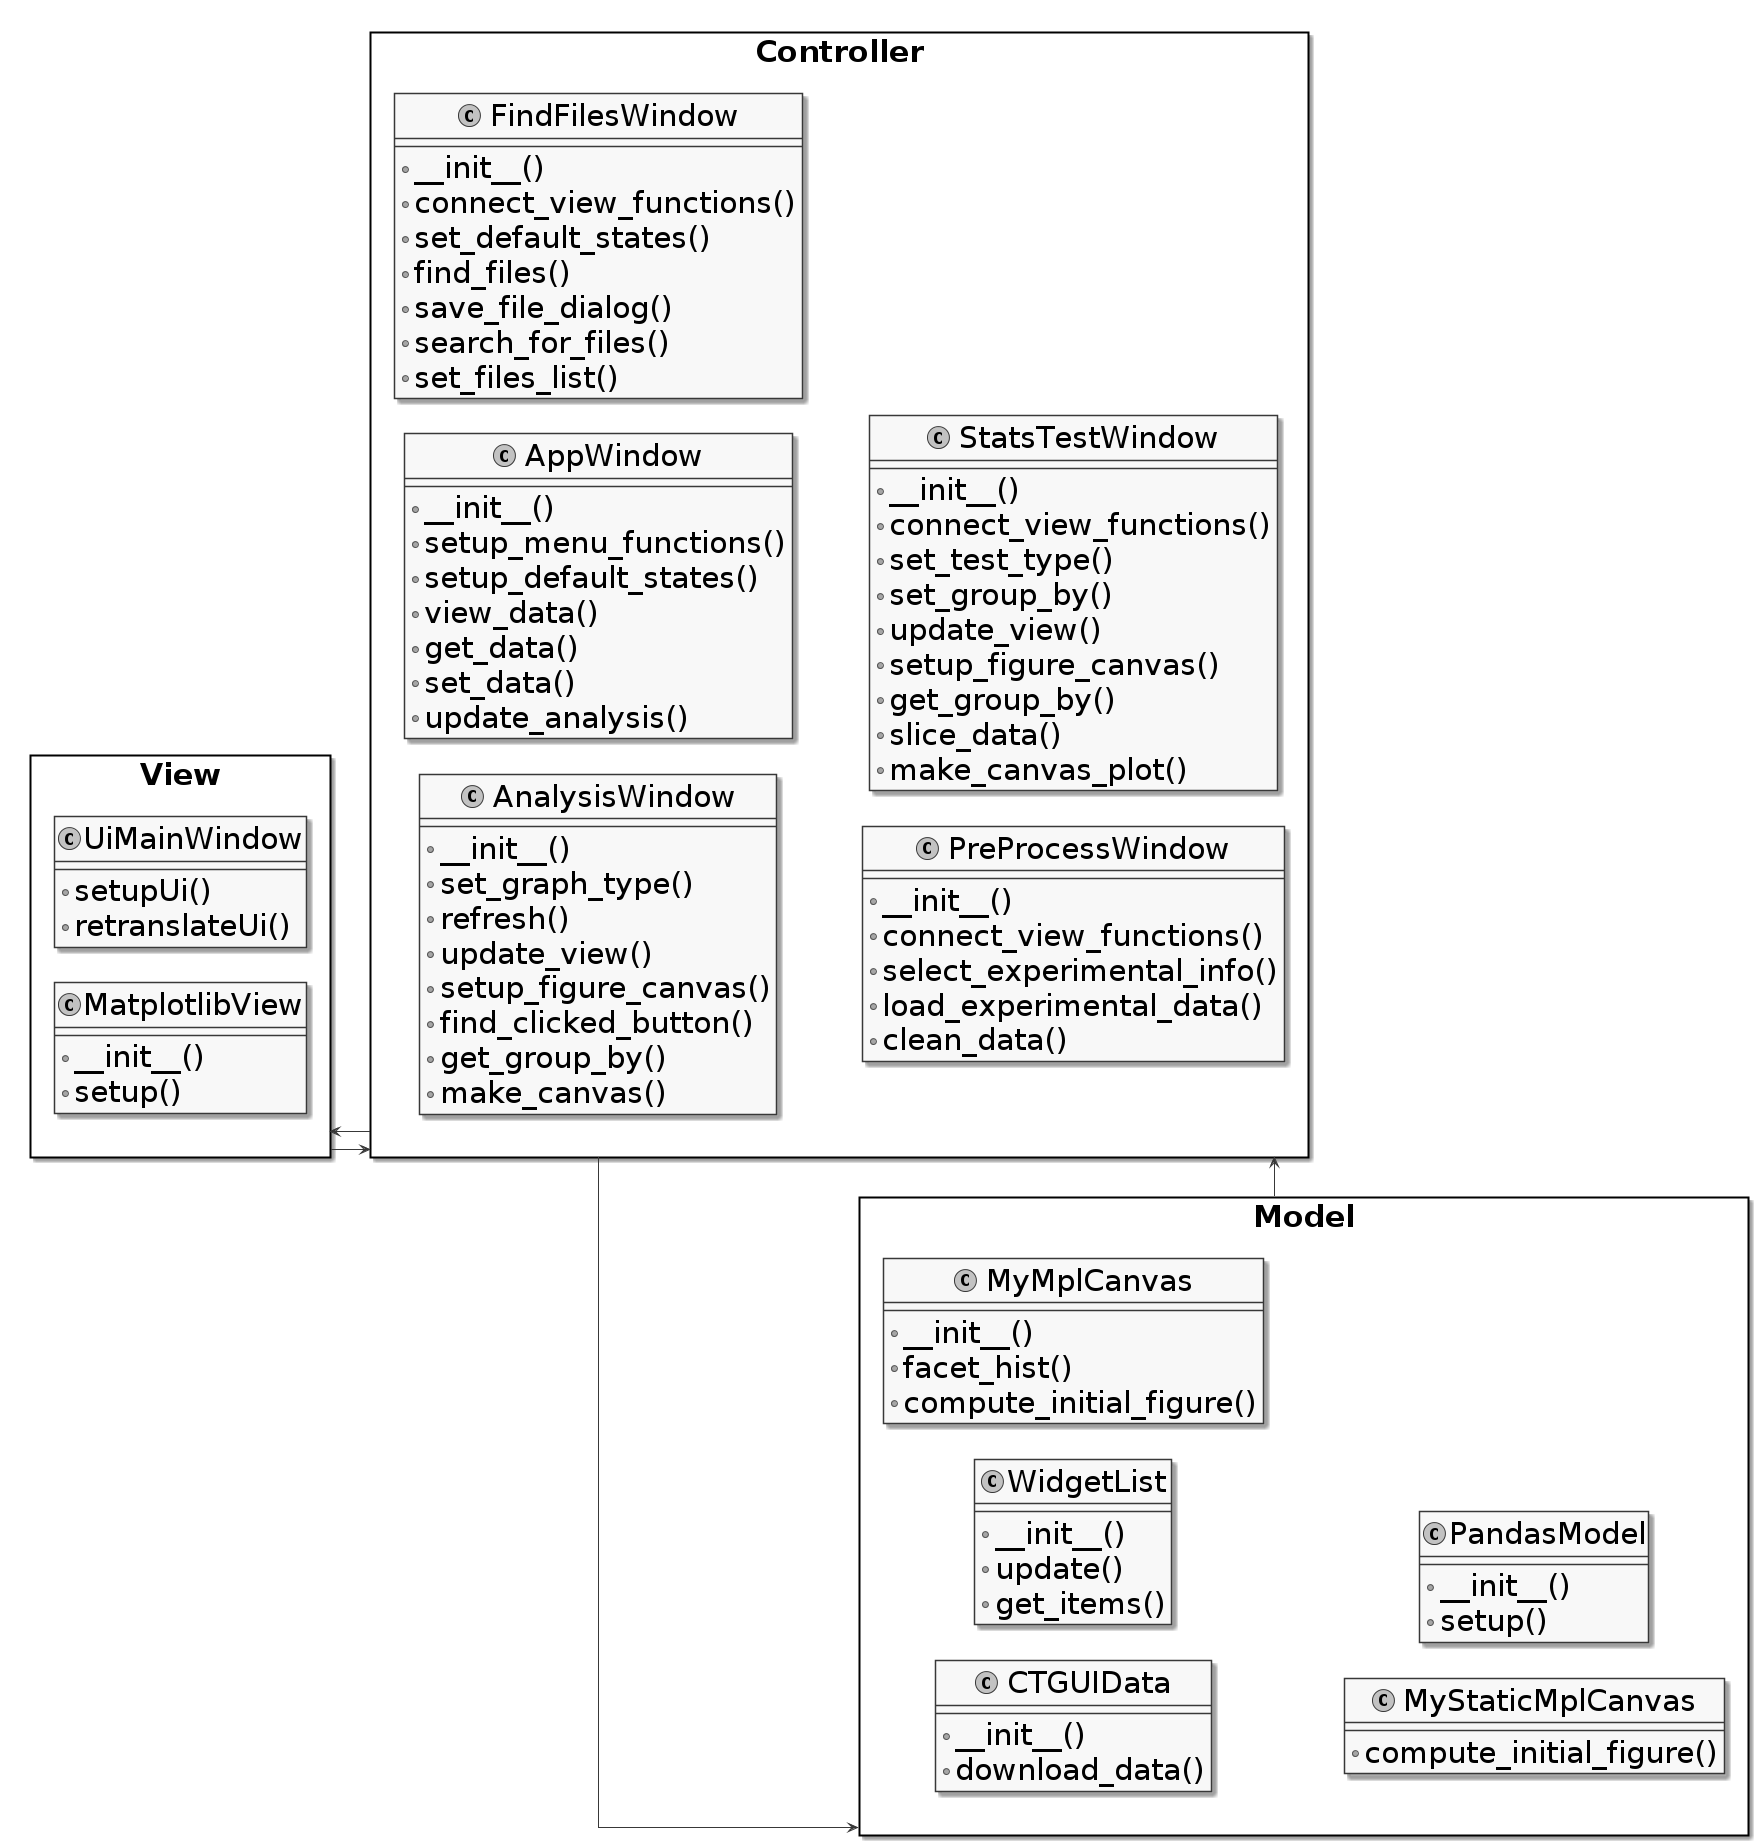
\includegraphics[width=15.2cm]{./images/ctgui.png}
\caption{\label{fig:orgfd5c317}
CT Analysing GUI UML}
\end{figure}
\section{Library Versioning}
\label{sec:org664dca2}
The development of this project was performed using the Python \emph{virtualenv}. This is a virtual environment package which Python offers, it allows for an isolated working copy of the project.

By developing in this manner, libraries were ensured to be using the correct versions required by the software.
 \clearpage
\section{Testing}
\label{sec:org8b532c5}
Testing was performed both in acceptance testing by using user feedback, the functional requirements and the ability to use the software to answer the hypothesis of the research elements of this project. Further to this, unit testing was performed to allow for automated testing as well as test-driven-development of features.
\subsection{Feedback Forms}
\label{sec:org8307c7c}
Feedback and constructive suggestions were made by researchers at the National Plant Phenomics Centre, these were submitted via the Google forms service.

These provided a method of acceptance testing by those who would be using the software to help with investigating data. Page 1 of the given form is shown in figure:\ref{fig:org0cc9015}. This form was completed by 3 researchers at the National Plant Phenomics Centre, feedback was very positive overall.
\begin{figure}[htbp]
\centering
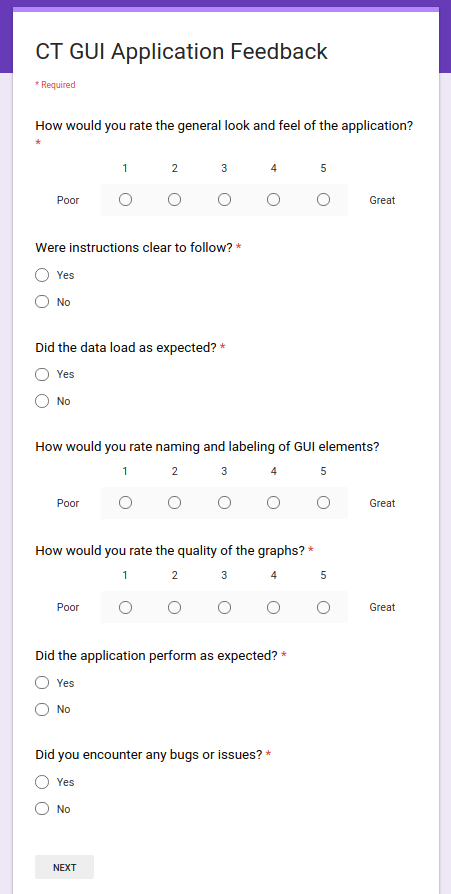
\includegraphics[width=7.3cm]{./images/feedbackform.png}
\caption{\label{fig:org0cc9015}
CT Feedback form}
\end{figure}

\clearpage

\subsection{Unit Testing CT Analysing Library}
\label{sec:org9f05182}
The unit tests for the CT Analysing Library were straightforward, using the \emph{PyTest} framework and a subset of data from a data set, these tests assert that features are implemented correctly and that the correct results are given.


\begin{table}[htbp]
\caption{\label{tab:orgbe5bfa9}
Output of \emph{pytest} Unit Tests and results for CT Analysing Library}
\centering
\begin{tabularx}{\textwidth}{|l|l|X|}
\hline
\textbf{I.D.} & \textbf{Result} & \textbf{Test}\\
\hline
0 & Passed & CTData.py::test\_aggregate\_spike\_averages\\
\hline
1 & Passed & CTData.py::test\_clean\_data\_maximum\_removed\\
\hline
2 & Passed & CTData.py::test\_clean\_data\_minimum\_removed\\
\hline
3 & Passed & CTData.py::test\_load\_additional\_data\\
\hline
4 & Passed & CTData.py::test\_load\_additional\_data\_no\_data\\
\hline
5 & Passed & CTData.py::test\_load\_data\\
\hline
6 & Passed & CTData.py::test\_NoDataFoundException\\
\hline
7 & Passed & Data\_transforms.py::test\_box\_cox\_data\\
\hline
8 & Passed & Data\_transforms.py::test\_pca\_to\_table\\
\hline
9 & Passed & Data\_transforms.py::test\_perform\_pca\\
\hline
10 & Passed & Data\_transforms.py::test\_standardise\_data\\
\hline
11 & Passed & Graphing.py::test\_plot\_boxplot\_as\_dataframe\\
\hline
12 & Passed & Graphing.py::test\_plot\_boxplot\_as\_object\\
\hline
13 & Passed & Graphing.py::test\_plot\_difference\_of\_means\\
\hline
14 & Passed & Graphing.py::test\_plot\_histogram\_as\_dataframe\\
\hline
15 & Passed & Graphing.py::test\_plot\_histogram\_as\_object\\
\hline
16 & Passed & Graphing.py::test\_plot\_pca\\
\hline
17 & Passed & Graphing.py::test\_plot\_qqplot\\
\hline
18 & Passed & Statistical\_tests.py::test\_baysian\_hypothesis\_test\\
\hline
19 & Passed & Statistical\_tests.py::test\_t\_test\\
\hline
20 & Passed & Statistical\_tests.py::test\_test\_normality\\
\hline
\end{tabularx}
\end{table}


\clearpage

\subsection{Unit Testing CT GUI Application}
\label{sec:org3ffd5c0}

The unit testing used for the CT GUI Application was more sophisticated than that of the Library. This testing required visual confirmation that figures and graphs generated were displayed correctly and that they showed what the user would expect, given the data.

To do this a \emph{PyTest} plugin was used, \emph{QtBot} which provides simulated user input. This allows for the GUI to be thoroughly tested, automatically.

In table:\ref{tab:org7fc80f7} the results of the automated testing is given along side an image of several of the tests, tests of the same graphs but with different parameters were also generated and manually verified and provided as supplemental data.

\begin{longtable}{|l|l|p{4.4cm}|C|}
\caption{\label{tab:org7fc80f7}
Output of \emph{pytest} Unit Tests and results for CT GUI Application}
\\
\hline
\textbf{I.D.} & \textbf{Result} & \textbf{Test} & \textbf{Image}\\
\hline
\endfirsthead
\multicolumn{4}{l}{Continued from previous page} \\
\hline

\textbf{I.D.} & \textbf{Result} & \textbf{Test} & \textbf{Image} \\

\hline
\endhead
\hline\multicolumn{4}{r}{Continued on next page} \\
\endfoot
\endlastfoot
\hline
21 & Passed & analysis.py:: box\_groupby\_1\_rb\_1 & \begin{center}
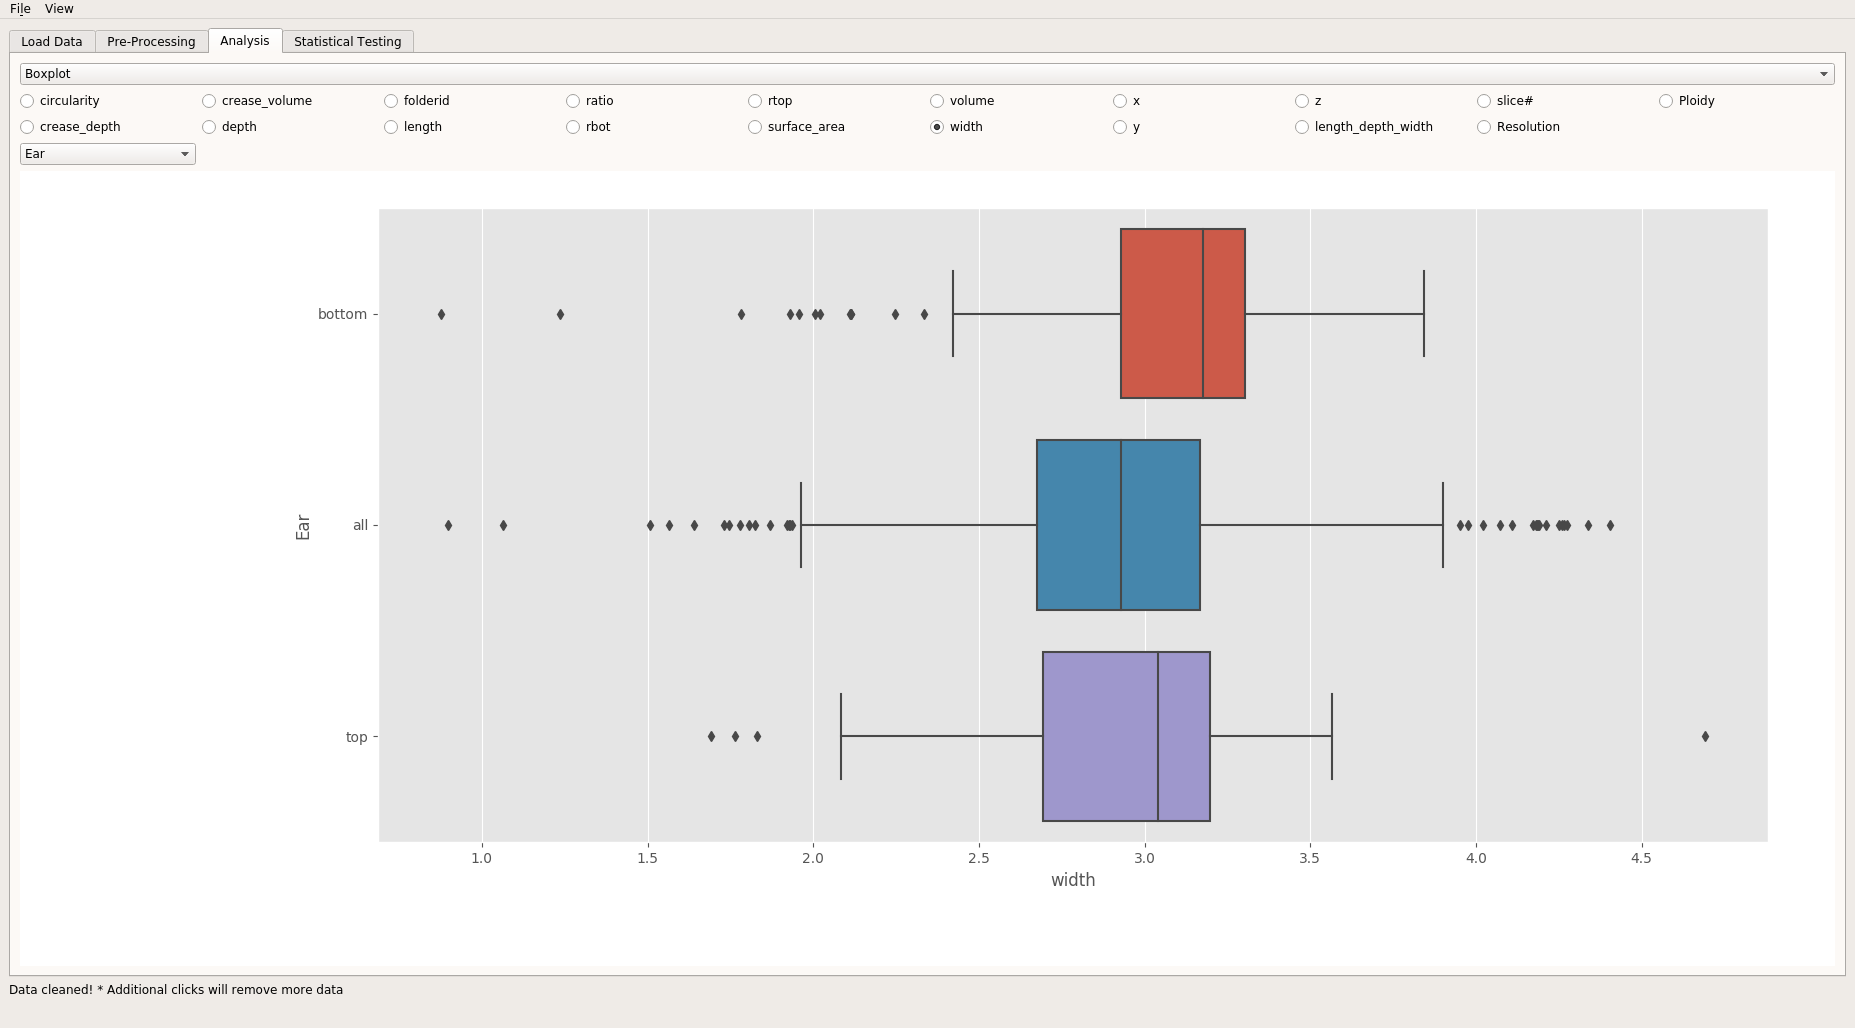
\includegraphics[width=.9\linewidth]{./images/Screenshots/analysis_window_box_groupby_1_rb_1.png}
\end{center}\\
\hline
22 & Passed & analysis.py:: box\_groupby\_2\_rb\_2 & \begin{center}
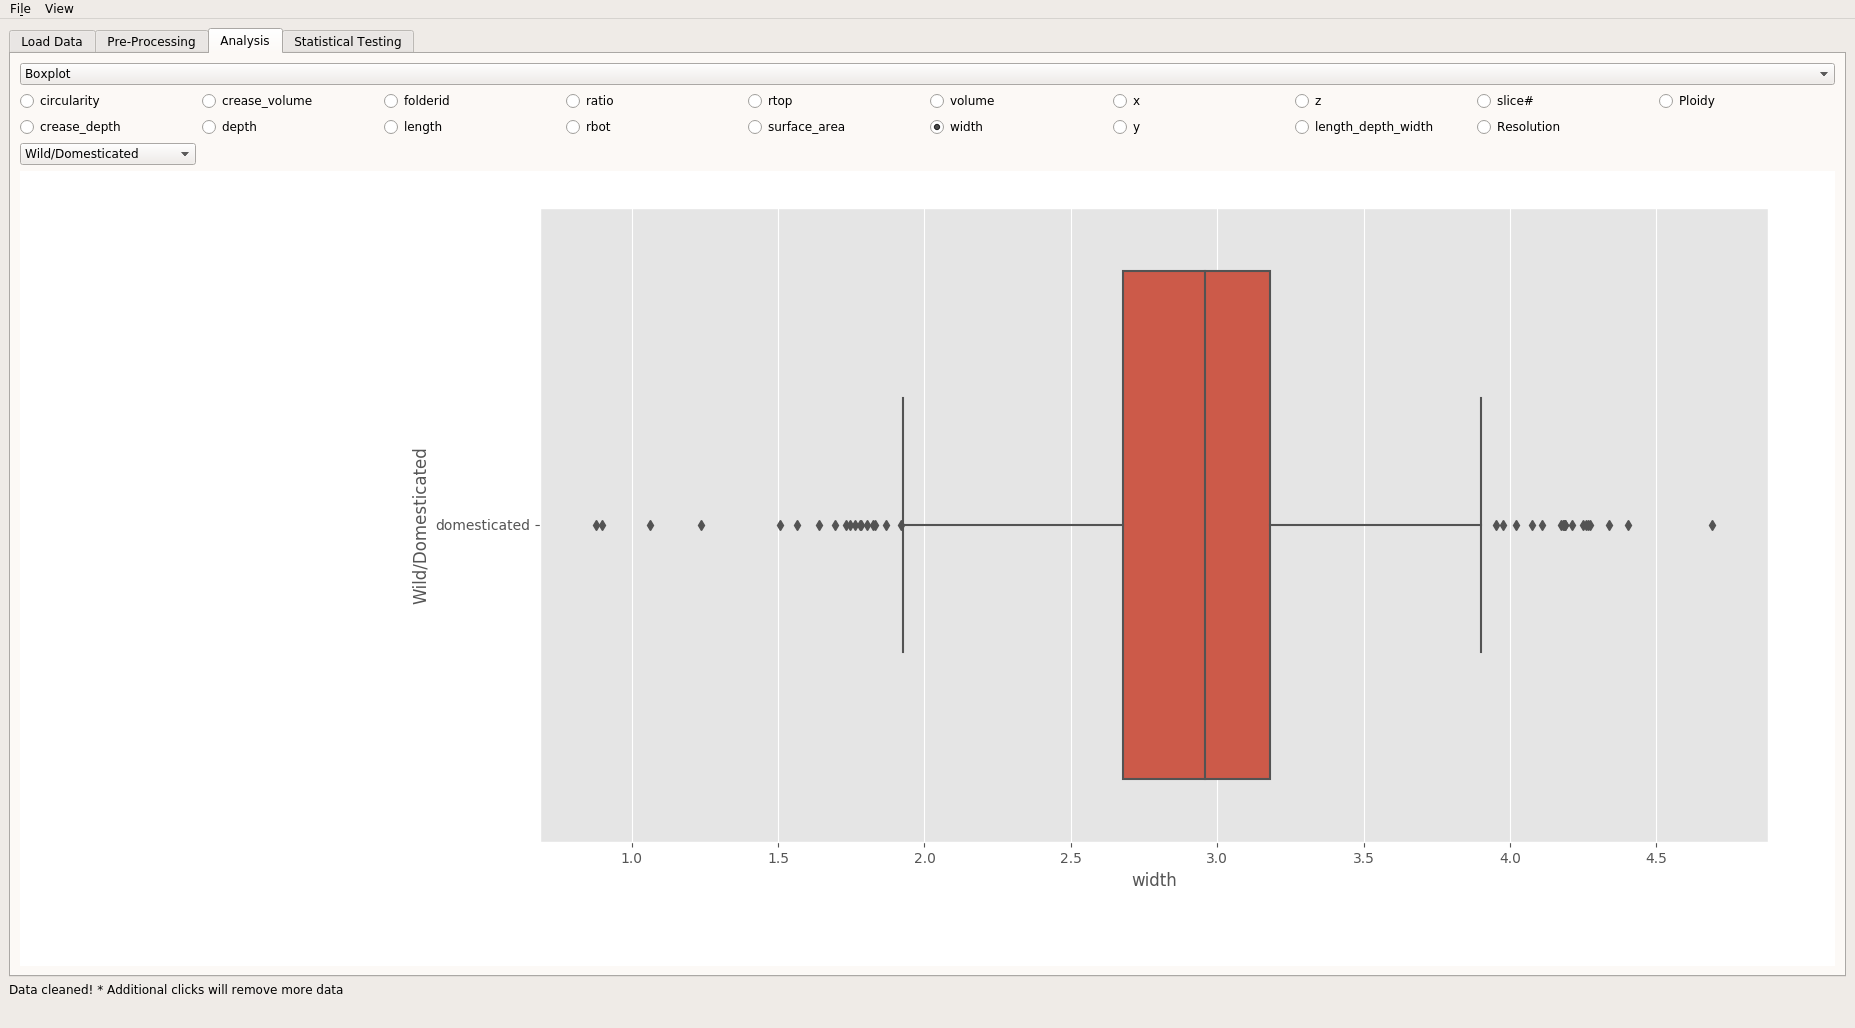
\includegraphics[width=.9\linewidth]{./images/Screenshots/analysis_window_box_groupby_2_rb_2.png}
\end{center}\\
\hline
23 & Passed & analysis.py:: box\_rb\_1 & \begin{center}
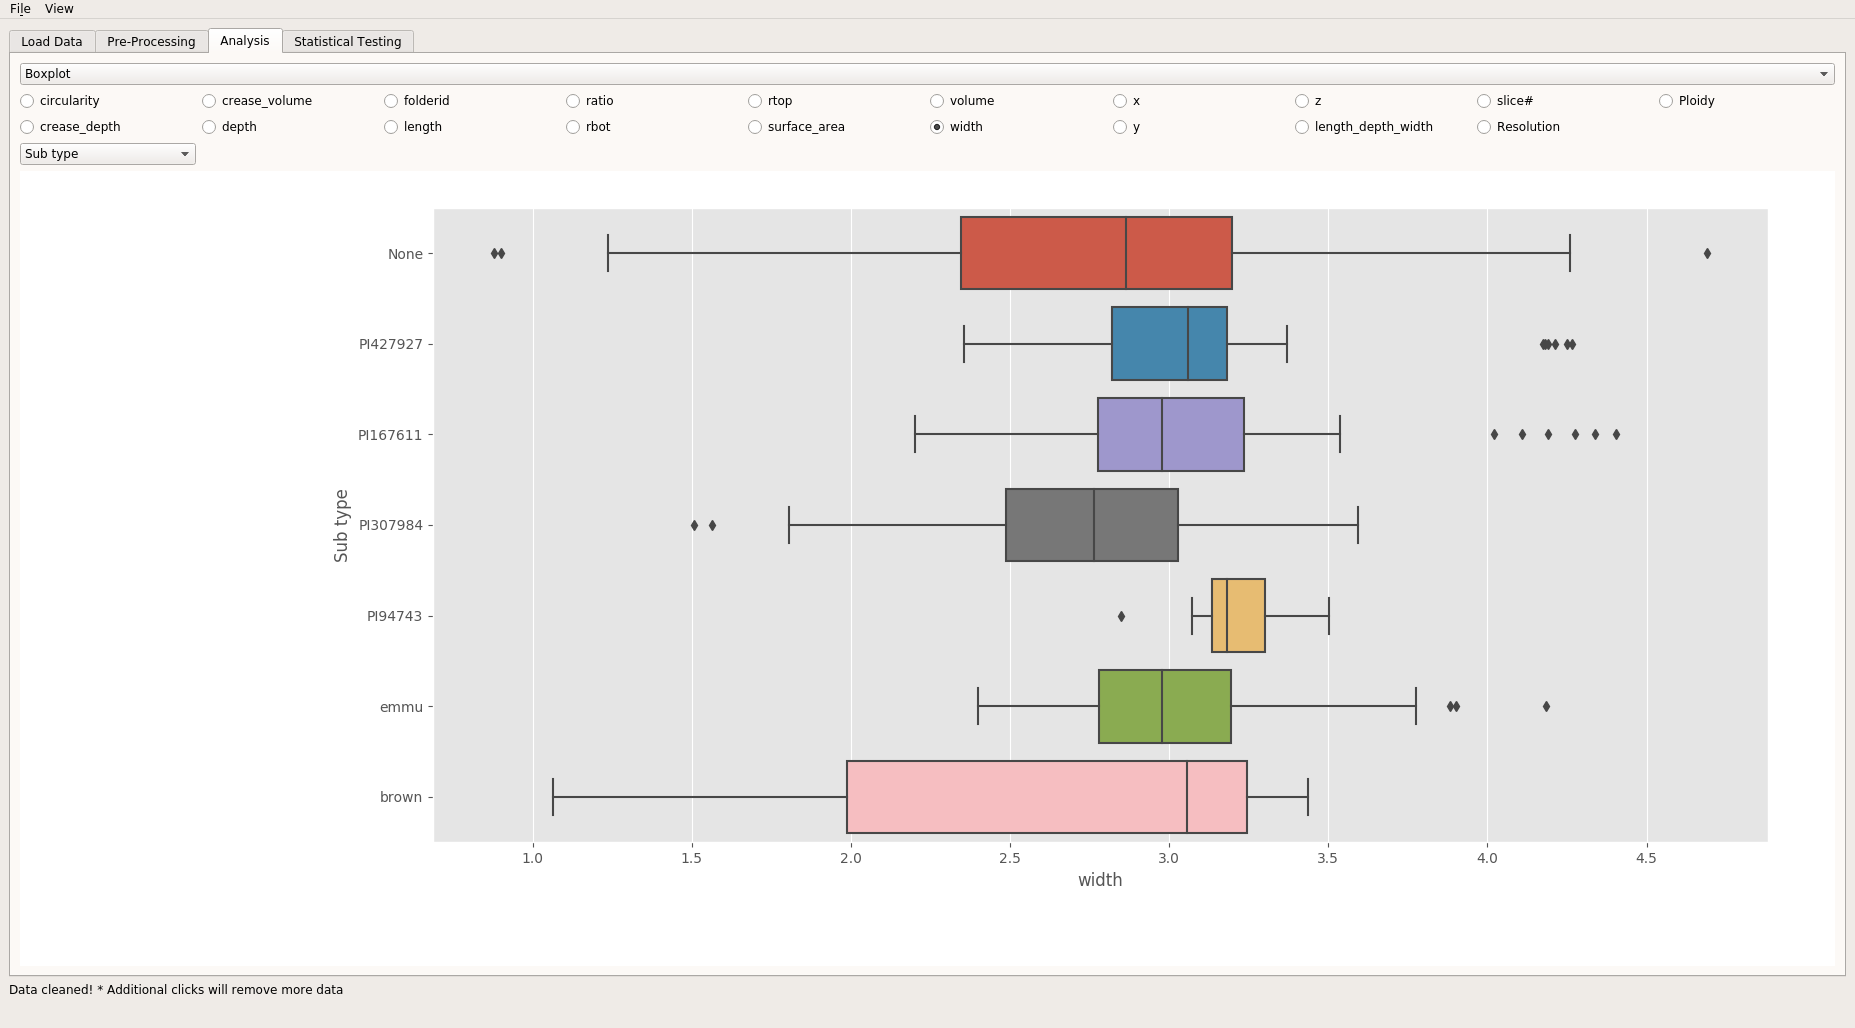
\includegraphics[width=.9\linewidth]{./images/Screenshots/analysis_window_box_rb_1.png}
\end{center}\\
\hline
24 & Passed & analysis.py:: hist\_groupby\_1\_rb\_1 & \begin{center}
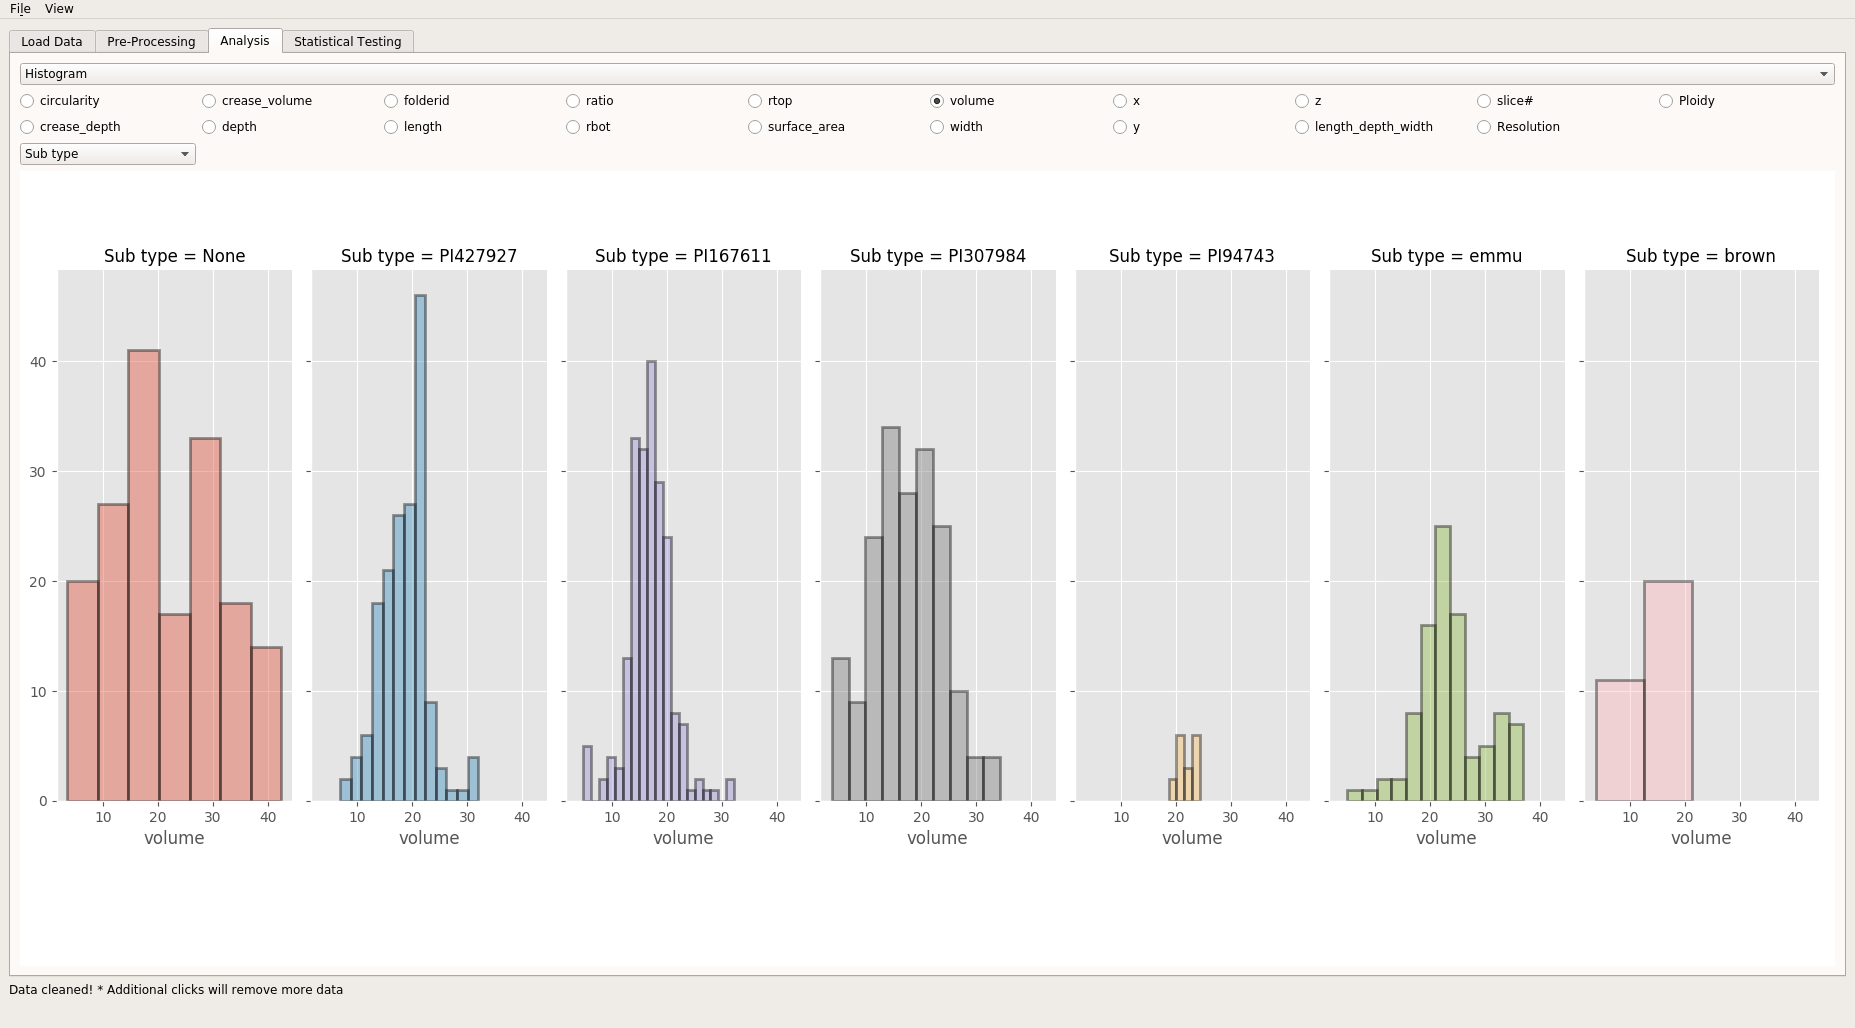
\includegraphics[width=.9\linewidth]{./images/Screenshots/analysis_window_hist_groupby_1_rb_1.png}
\end{center}\\
\hline
25 & Passed & analysis.py:: hist\_rb\_1 & \begin{center}
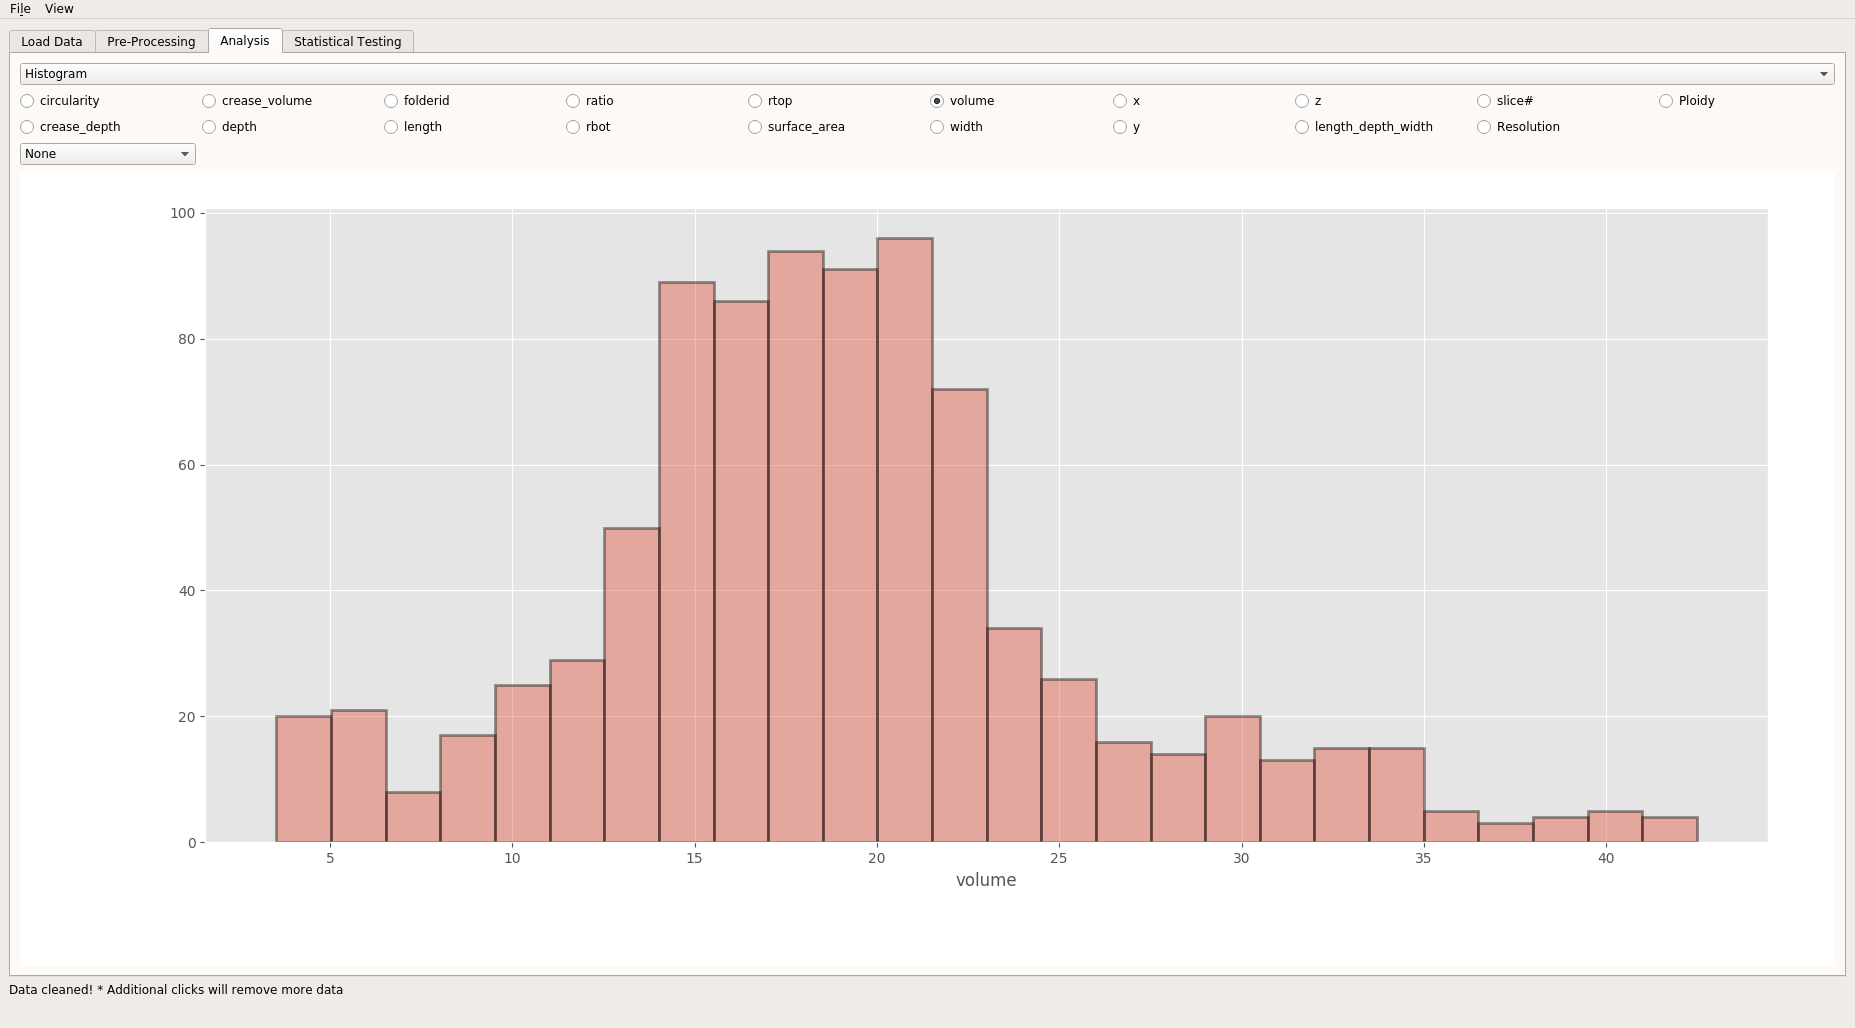
\includegraphics[width=.9\linewidth]{./images/Screenshots/analysis_window_hist_rb_1.png}
\end{center}\\
\hline
26 & Passed & hypothesis\_tests.py:: bayesg1\_att\_1 & \begin{center}
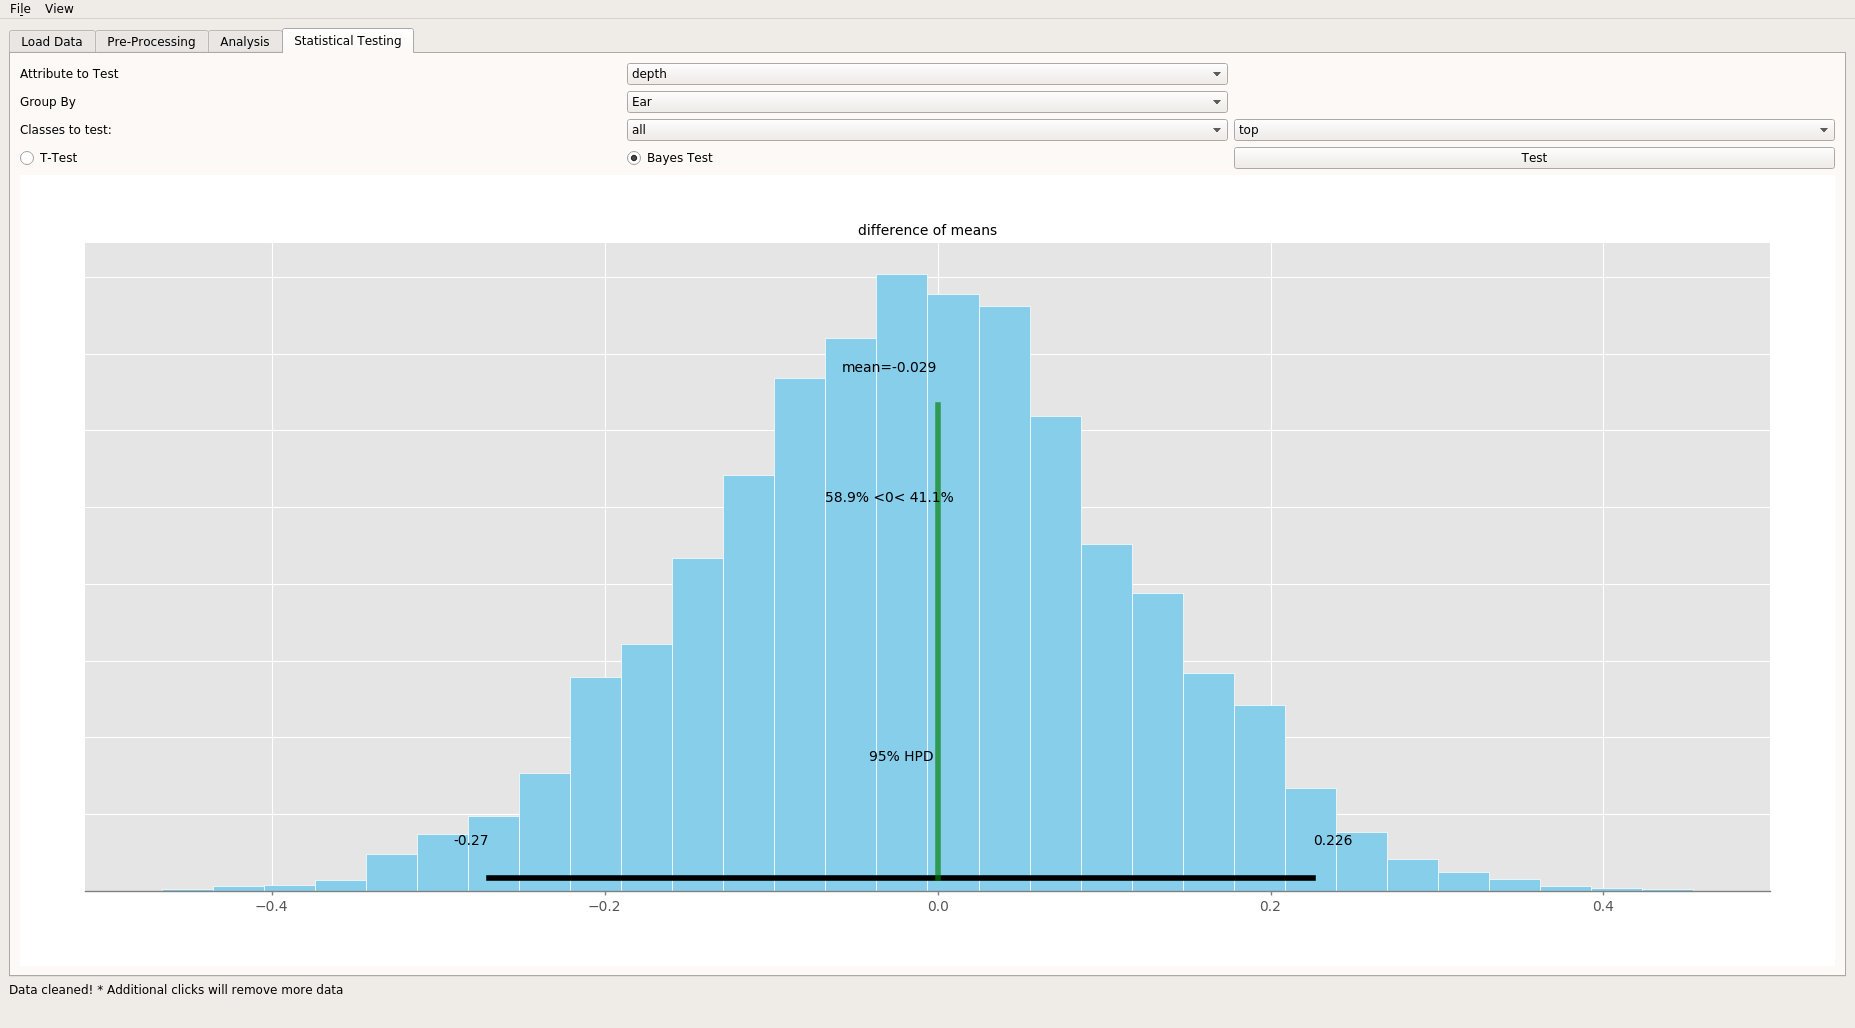
\includegraphics[width=.9\linewidth]{./images/Screenshots/hypothesis_bayestest_g1_att_1.png}
\end{center}\\
\hline
27 & Passed & hypothesis\_tests.py:: tg1\_att\_1 & \begin{center}
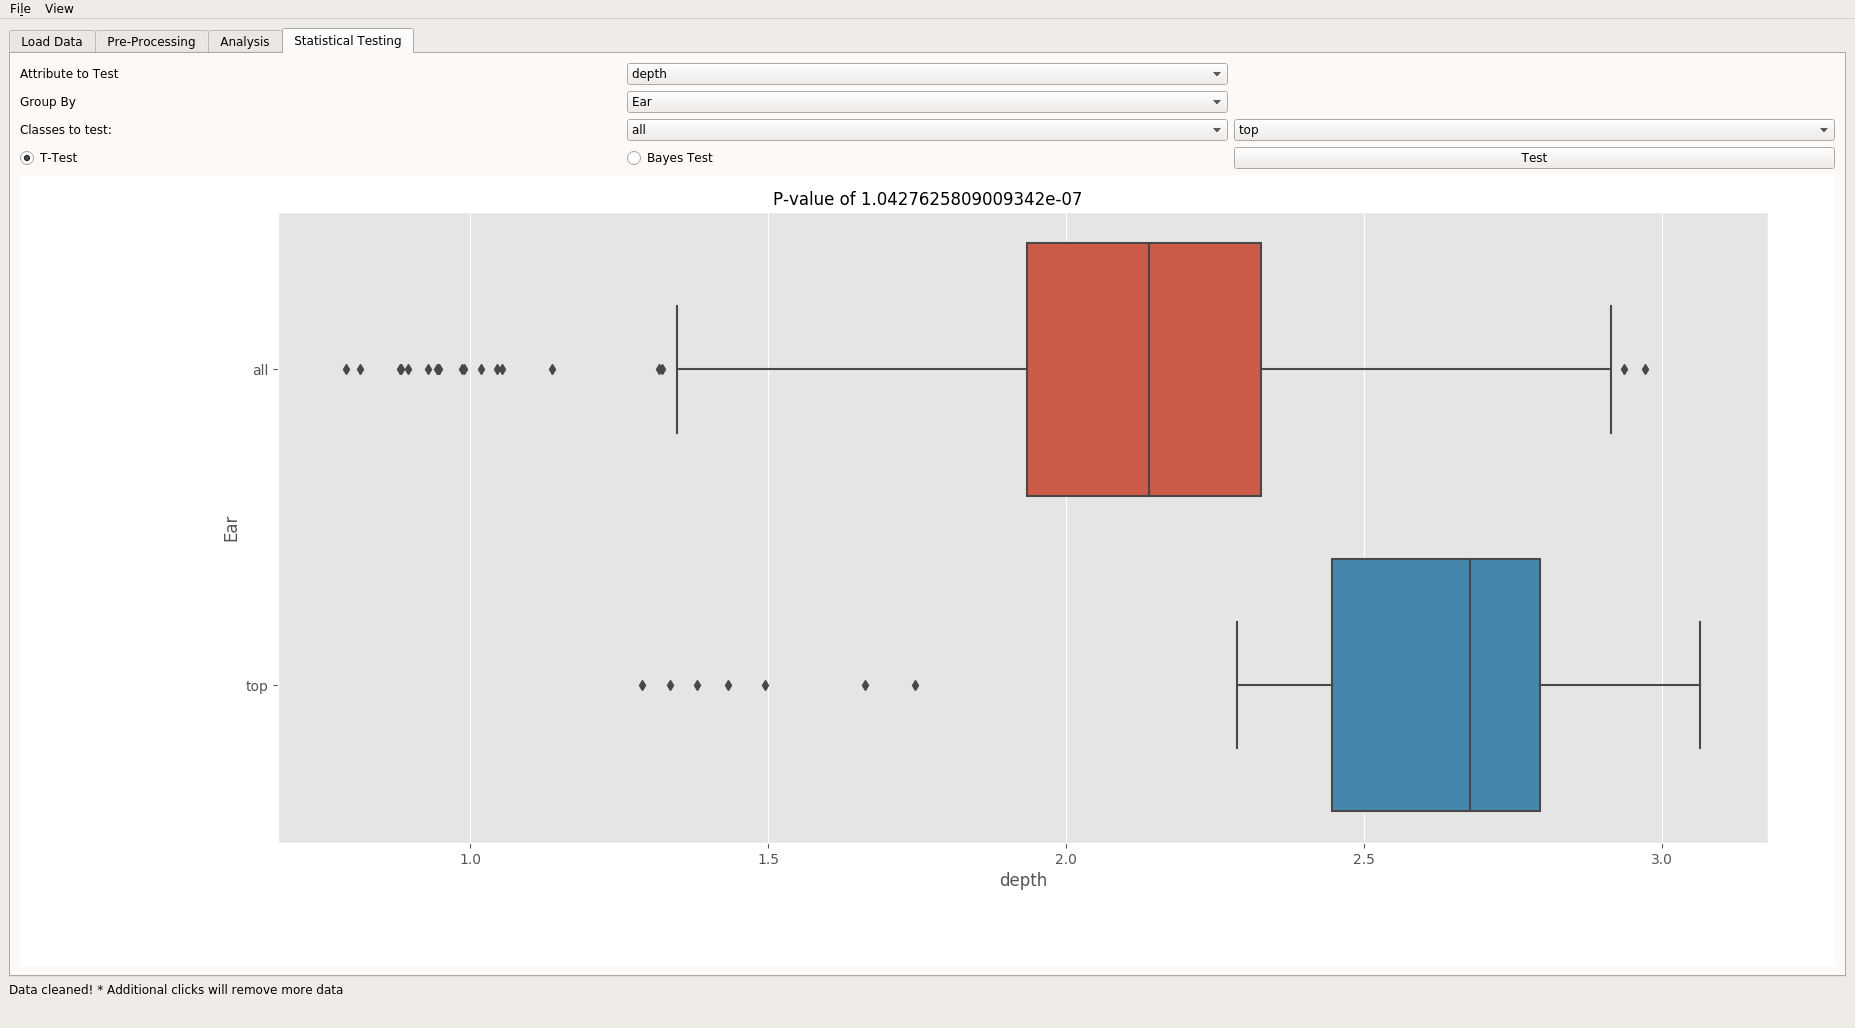
\includegraphics[width=.9\linewidth]{./images/Screenshots/hypothesis_ttest_g1_att_1.png}
\end{center}\\
\hline
28 & Passed & analysis.py:: box\_rb\_2 & N/A\\
\hline
29 & Passed & analysis.py:: hist\_groupby\_1\_rb\_2 & N/A\\
\hline
30 & Passed & analysis.py:: hist\_rb\_2 & N/A\\
\hline
31 & Passed & analysis.py:: loads & N/A\\
\hline
32 & Passed & hypothesis\_tests.py:: bayesg1\_att\_2 & N/A\\
\hline
33 & Passed & hypothesis\_tests.py:: bayesg2\_att\_1 & N/A\\
\hline
34 & Passed & hypothesis\_tests.py:: bayesg2\_att\_2 & N/A\\
\hline
35 & Passed & hypothesis\_tests.py:: tg1\_att\_2 & N/A\\
\hline
36 & Passed & hypothesis\_tests.py:: tg2\_att\_1 & N/A\\
\hline
37 & Passed & hypothesis\_tests.py:: tg2\_att\_2 & N/A\\
\hline
38 & Passed & hypothesis\_tests.py:: loads & N/A\\
\hline
39 & Passed & GUI.py:: startup & N/A\\
\hline
40 & Passed & load\_data.py:: load\_data\_with\_rachis & N/A\\
\hline
41 & Passed & load\_data.py:: load\_data\_without\_rachis & N/A\\
\hline
42 & Passed & preprocessing.py:: clean\_data\_remove\_large & N/A\\
\hline
43 & Passed & preprocessing.py:: clean\_data\_remove\_none & N/A\\
\hline
44 & Passed & preprocessing.py:: clean\_data\_remove\_small & N/A\\
\hline
45 & Passed & preprocessing.py:: clean\_data\_remove \_small\_and\_large & N/A\\
\hline
46 & Passed & preprocessing.py:: load\_additional\_data & N/A\\
\hline
47 & Passed & preprocessing.py:: load\_additional\_data \_expected\_fail & N/A\\
\hline
\end{longtable}

\subsection{Acceptance Testing}
\label{sec:orgd1b1f32}
These unit tests, alongside user tests have been used to meet the outlined functional requirements; specific tests are shown in table:\ref{tab:org51e9c82} to match them to the associated functional requirement.

\begin{longtable}{|l|l|p{14cm}|}
\caption{\label{tab:org51e9c82}
Functional requirements and Unit tests}
\\
\hline
\textbf{F.R.} & \textbf{U.T.} & \textbf{How is the F.R. met?}\\
\hline
\endfirsthead
\multicolumn{3}{l}{Continued from previous page} \\
\hline

\textbf{F.R.} & \textbf{U.T.} & \textbf{How is the F.R. met?} \\

\hline
\endhead
\hline\multicolumn{3}{r}{Continued on next page} \\
\endfoot
\endlastfoot
\hline
0 & n/a & An OOP interface is provided by the \emph{ct\_data} object\\
\hline
1 & 3,4,5 & Loading of data is tested multiple times specifically through unit tests\\
\hline
2 & 4,5 & Unit tests carry out saving loaded data into appropriate formats, in particular python \emph{pandas} tables and CSV files, this was also user tested\\
\hline
3 & 7,8,9,10 & All the functions in the \emph{data\_transforms.py} library are unit tested automatically on test data of known output\\
\hline
4 & 26,27,32-38 & Hypothesis testing was tested with known data 8+ times in automated unit testing for both CT GUI Application and the CT Analysis Library group of tests , testers also used these functions\\
\hline
5 & 6,7 & Loading of spikes was tested both for data which was known to exist and could be successfully done, and for data which was know to throw errors\\
\hline
6 & 1,2,7,42-46 & Finding and removing erroneous data was unit tested by having a combination of parameters tested for both the GUI and the Analysis Library\\
\hline
7 & 3-6,40,41 & Matching of pre-existing experiment information to the extracted data was tested for bad inputs through unit testing, users tested this too and reported no unexpected results\\
\hline
8 & 11-17,28-38 & Plotting of data automatically, inferring of axis, titles and measurements was tested, with images automatically recorded by unit tests.\\
\hline
9 & 0,1,2,3 & Unit testing checked if given data could easily be separated and divided into subsections, this was specifically tested and tested by proxy in other tests when hypothesis testing was performed\\
\hline
10 & 21,26 39,40,42 & Multiple tests are taken to check that the GUI loads as expected, planning sessions and user feedback was also used to meet this particular functional requirement\\
\hline
11 & 40,42 & Data is loaded through GUI elements with little prior knowledge of the software in order to have data processed, this was unit tested and user feedback was used to make more accessible\\
\hline
12 & 21-27 & Testing of \emph{Matplotlib} and \emph{Seaborn} interfacing with, and integrating with the CT Analysing GUI.\\
\hline
13 & 43-47 & Loading of experiment data is pivotal for most functionality of the GUI, it is tested multiple times in an isolated formatted, as well as by other future functions which require it\\
\hline
14 & n/a & The entire software is wrapped in an MVC model, this cannot be tested but the functional requirement has been met\\
\hline
15 & 21-47 & All of the unit tests for the CT Analysing GUI depend on the CT Analysing Library, it is reasonable that the integration is well tested, by product of all other tests\\
\hline
16 & 21-27 & Several tests, those shown in table:\ref{tab:org7fc80f7} are specifically recorded visually and presented as images in order to automatically unit test that visual data is intact\\
\hline
17 & 21-27 & By using automatic image capturing of unit testing in progress, visual checking can be carried out and confirmed that data is visually what is expected and to a high standard\\
\hline
18 & 26,27, 32-28 & With multiple known outputs, several different groupings and combinations the hypothesis tests were unit tested and this functional requirement is known to be acceptably implemented\\
\hline
\end{longtable}

\chapter{Methods and Solutions}
\label{sec:org5704188}
This chapter will discuss and expand upon the software implementations which were carried out in the course of this project, with particular focus on novel and non-trivial elements of software engineering.

Where appropriate code segments are provided to illustrate how a feature has been implemented in software.

\section{Data Processing Methods}
\label{sec:org42efe4d}
This project presents a start to finish style of data analysis, data are generated by extracting information from raw scans, the resulting data is then post-processed and statistical analysis draws information from this.

Historically, these processes and tasks are huge time sinks in terms of manual work, this project emphasises an increase in automation.

Two separate pipelines are provided to carry out these tasks.

\subsection{Image-Data Requisition Pipeline}
\label{sec:orgfdc4baf}

Acquiring data for this study first required Wheat plants to be grown and harvested, the process outlined here begins with scanning samples from these plants in a \textmu{}-CT machine.

These scans are processed by MATLAB \cite{MATHWORKS2017}. This process is defined as a method by Hughes et al. \cite{Hughes2017}, new and novel additions are added in the watershedding and segmentation processes.

The process begins by loading the scans into greyscale images, the pixel values (which translate to density values) are used to calculate a threshold that is used to define and segment material of interest (seeds).

Due to the low resolution of the imaging technique (68.6\textmu{} meters per pixel) objects can appear connected which are not, a three dimensional watershedding algorithm is used to correct any objects which appear connected when they should not be.

Finally, each isolated object is exported for measuring (objects are defined by groups of connected pixels), measurements are recorded into tables and saved as CSV files. The data is recorded as pixel values and converted to appropriate real-world measurements.

The entire process is represented as a diagram in figure:\ref{fig:org00c86e5}

\begin{figure}[htbp]
\centering
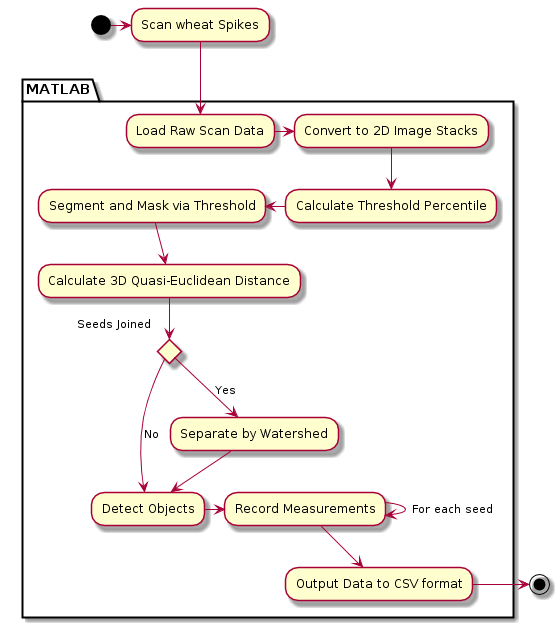
\includegraphics[width=15cm]{./images/matlab.png}
\caption{\label{fig:org00c86e5}
Image Processing Pipeline}
\end{figure}

\subsection{Morphometric Features}
\label{sec:orgdb76a91}

The features/phenotypes used are extracted during the imaging process.
\begin{itemize}
\item Length is calculated using the major axis of the whole grain.
\item Width and depth are the major and minor axis of a cross section, found by selecting the grain's midpoint.
\item Volume is a complete connected pixel count per grain
\item Surface area is a single pixel perimeter calculation mapped in 3 dimensions
\item Length X Depth X Width is a post-image-processing value calculated by the interaction between the three dimension descriptors.
\end{itemize}

Values used in statistical functions and measurements are presented as metric units, derived from \textmu{}-CT image pixel values. The equation:\ref{eq:orge17ff34} is presented here.

\begin{align}
\label{eq:orge17ff34}
  &\begin{aligned}
mm = \frac{pixel \times 68.8}{1000}
  \end{aligned}
\end{align}
\myequations{Pixel to metric milimeter conversion}


\subsection{Data Analysis Pipeline}
\label{sec:orgbc664e3}
The data analysis and research in this project is performed in part by automated software, the CT Analysis Library, and by human decision making as to statistical methods which need to be applied.

Here, the pipeline presented in figure:\ref{fig:orgbb38b02} demonstrates the process used by the CT Analysis Library, and by result the CT Analysing GUI.

The first stage of this process is loading in the data exported by the MATLAB software. These data are loaded on a per scan basis, meaning that the previously mentioned process of spike splitting is initially still an issue, a resulting \emph{CT Data} object is created, this holds the data and carries out the proper treatment for it.

The data needs to be checked for false positives, this is done by first removing outliers which are found by upper and lower percentiles of the data. Additionally constraints are applied to the data based on findings from previous studies \cite{Hughes2017}, this adds robustness.

When the data has been cleaned, additional data is added. The added data provides information about the experiment, plant names; genotypes; top and bottom scans. With this data, information on scans which need to be joined is provided.

Using data on \(x,y,z\) coordinates a approximation is made to join spikes at the most likely point at which they were initially cut for imaging.

An additional phenotype is created to describe the interaction between the geometric parameters; the interaction is described in equation:\ref{eq:org9f4b214}.

 \begin{align}
\label{eq:org9f4b214}
   &\begin{aligned}
\text{geometry interaction} = length \times depth \times width
   \end{aligned}
 \end{align}
\myequations{Pixel to metric milimeter conversion}

When data are usable columns can be aggregated to form averages, medians, standard deviations etc. on a per plant (sample) basis.

Finally, a decision is made by way of human input as to what type of statistics should be used to test hypothesis. This decision is mostly based on the distribution of the data where \(X \sim \mathcal{N}(\mu,\,\sigma^{2})\) data is tested with parametric tests (e.g. Student's T-Test) else non-parametric tests are used (e.g. Welch's T-Test).

From statistical testing a final result(s) can be used to answer scientific questions on the data. The entire process is represented in figure:\ref{fig:orgbb38b02}.
\clearpage
\begin{figure}[htbp]
\centering
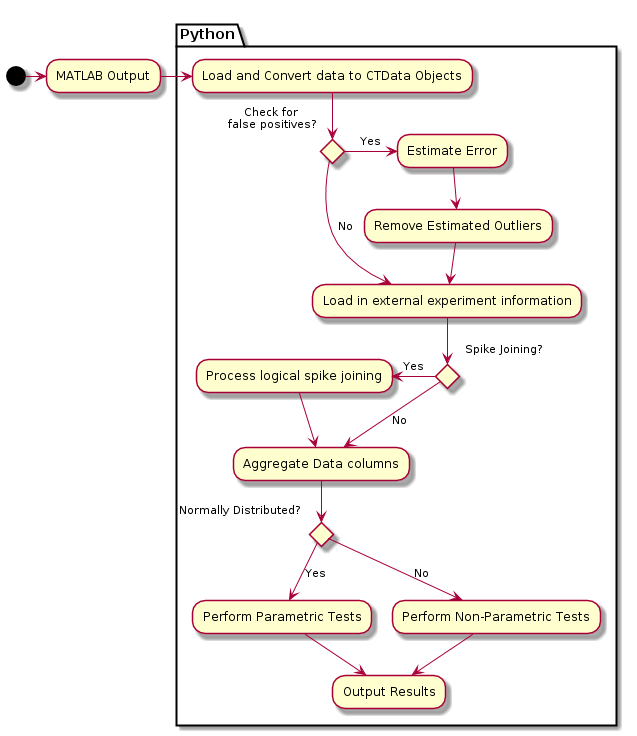
\includegraphics[width=18cm]{./images/pipeline.png}
\caption{\label{fig:orgbb38b02}
How data is integrated with the CT Analysing Library}
\end{figure}

\section{Image Analysis Methods}
\label{sec:org1cad466}
Initially, this project aimed to use existing software for feature extraction, however the range of data (due to the spectrum of genotypes in the study) meant that software which worked well for certain genotypes of wheat did not work well on others.

The issue became in seeds becoming erroneously joined, research and investigation lead to a new solution being implemented in a forked version of the open source software used for image analysis \cite{Hughes2017}

\subsection{New Watershed Algorithm}
\label{sec:orgba46190}

In order to solve the problem of misidentified and joint seeds, from the primitive collection,
a  \emph{quasi-euclidean} distance transform was implemented into the analysis pipeline (figure:\ref{fig:org00c86e5}). This provided much better results than the previous
\emph{chessboard} transform which had been successful on more uniform data in previous studies \cite{Hughes2017}.

\subsubsection{Quasi-Euclidean algorithm}
\label{sec:org2d5b820}

This algorithm measures the total euclidean distance along a set of horizontal, vertical and diagonal
line segments \cite{Pfaltz1966}.

\begin{align}
\label{eq:org0a035d4}
  &\begin{aligned}
&|x_1-x_2|+(\sqrt{2}-1)|y_1-y_2|, |x_1-x_2| > |y_1-y_2| \\
      &(\sqrt{2}-1)|x_1-x_2| + |y_1-y_2|, \textup{otherwise.}
  \end{aligned}
\end{align}
\myequations{Quasi-Euclidean Distance}

In order to apply this to a 3D space Kleinberg's method is used  \cite{Kleinberg1997}. This allows for nearest neighbour pixels to be sorted by \(k\) dimensional trees
and enabling fast distance transforms via Rosenfeld and Pfaltz's \emph{quasi-euclidean} method stated in equation:\ref{eq:org0a035d4}.

\subsection{Implementation}
\label{sec:orga4ee9f8}

The software implementation for this was done in MATLAB \cite{MATHWORKS2017}, this meant that it could instantly and easily be inserted into the existing pipeline in the open source software which was forked and modified to add this feature. In code listing:\ref{orgd81a0b2} this new algorithm, in full, is shown.

\begin{listing}[htbp]
\begin{minted}[linenos,firstnumber=1,frame=lines,linenos=true,fontfamily=DejaVuSans]{octave}
function [W] = watershedSplit3D(A)
  % Takes image stack A and splits it into stack W.
  % This is done by using a watershedding
  % algorithm based on quasi-euclidean distance

  % Convert to BW
  bw = logical(A);
  % Create variable for opening and closing
  se = strel('disk', 5);
  % Minimise object missshapen-ness
  bw = imerode(bw, se);
  bw = imdilate(bw, se);
  % Fill in any left over holes
  bw = imfill(bw,4,'holes');
  % Use chessboard for distance calculation for more refined splitting
  chessboard = -bwdist(~bw, 'quasi-euclidean');
  % Modify the intensity of our bwdist to produce chessboard2
  mask = imextendedmin(chessboard, 2);
  chessboard2 = imimposemin(chessboard, mask);
  % Calculate watershed based on the modified chessboard
  Ld2 = watershed(chessboard2);
  % Take original image and add on the lines calculated for splitting
  W = A;
  W(Ld2 == 0) = 0;
end
\end{minted}
\caption{\label{orgd81a0b2}
MATLAB Watershedding function}
\end{listing}

The process creates a black and white copy of the image, performs erosion and dilation to remove holes and erroneous pixels. A distance map is then created, this represents each pixel, which is plant material (grains), as an integer value of distance from the closest non-plant pixel. This map combines with the watershed algorithm to provide an estimate of where objects are incorrectly connected (fused grains), subtracting this from the original 3D image provides cleaning split and segmented grains which can be passed through to the next stage of the pipeline.

\subsubsection{Reasons for Improvement}
\label{sec:org5bb21a6}

This improved algorithm for measuring distance between points works well with this data because of the variation in seed morphology.

Where previous studies \cite{Hughes2017} found their methods worked well, they also used elite well-bred wheat varieties. These varieties have a more round more even shape with a low standard deviation in shape, generally.

This study, with such a varied group of genotypes has encountered many seeds which do not have a reasonable degree of regularity in shape. As such, a simple distance based method of splitting from the centre of objects was ill suited. By using a quasi-euclidean distance a more flexible shape is afforded in grains and the resulting segmentation is less prone to over-zealous splitting due to non-uniform shape.

\subsubsection{Effect of Enhanced Watershed algorithm in 2D}
\label{sec:orga918651}

Figure:\ref{fig:org6ee021c} shows in two dimensional flat images how this problem was solved. As well as what the previous method was doing to cause errors in data.
\begin{figure}[htbp]
\centering
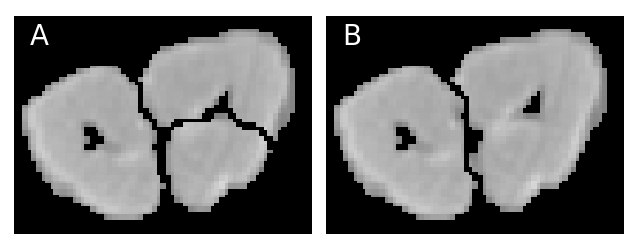
\includegraphics[width=16cm]{./images/chess_quasi.png}
\caption{\label{fig:org6ee021c}
\emph{A} showing the chessboard method, \emph{B} improved quasi-euclidean method}
\end{figure}

\clearpage
\subsubsection{Effect of Enhanced Watershed algorithm in 3D}
\label{sec:org7f79f49}

Figure:\ref{fig:org56eafe0} shows the effects on grains in three dimensions, where the seeds which where incorrectly split have now been vastly improved, leading to an increase in result accuracy.

\begin{figure}[htbp]
\centering
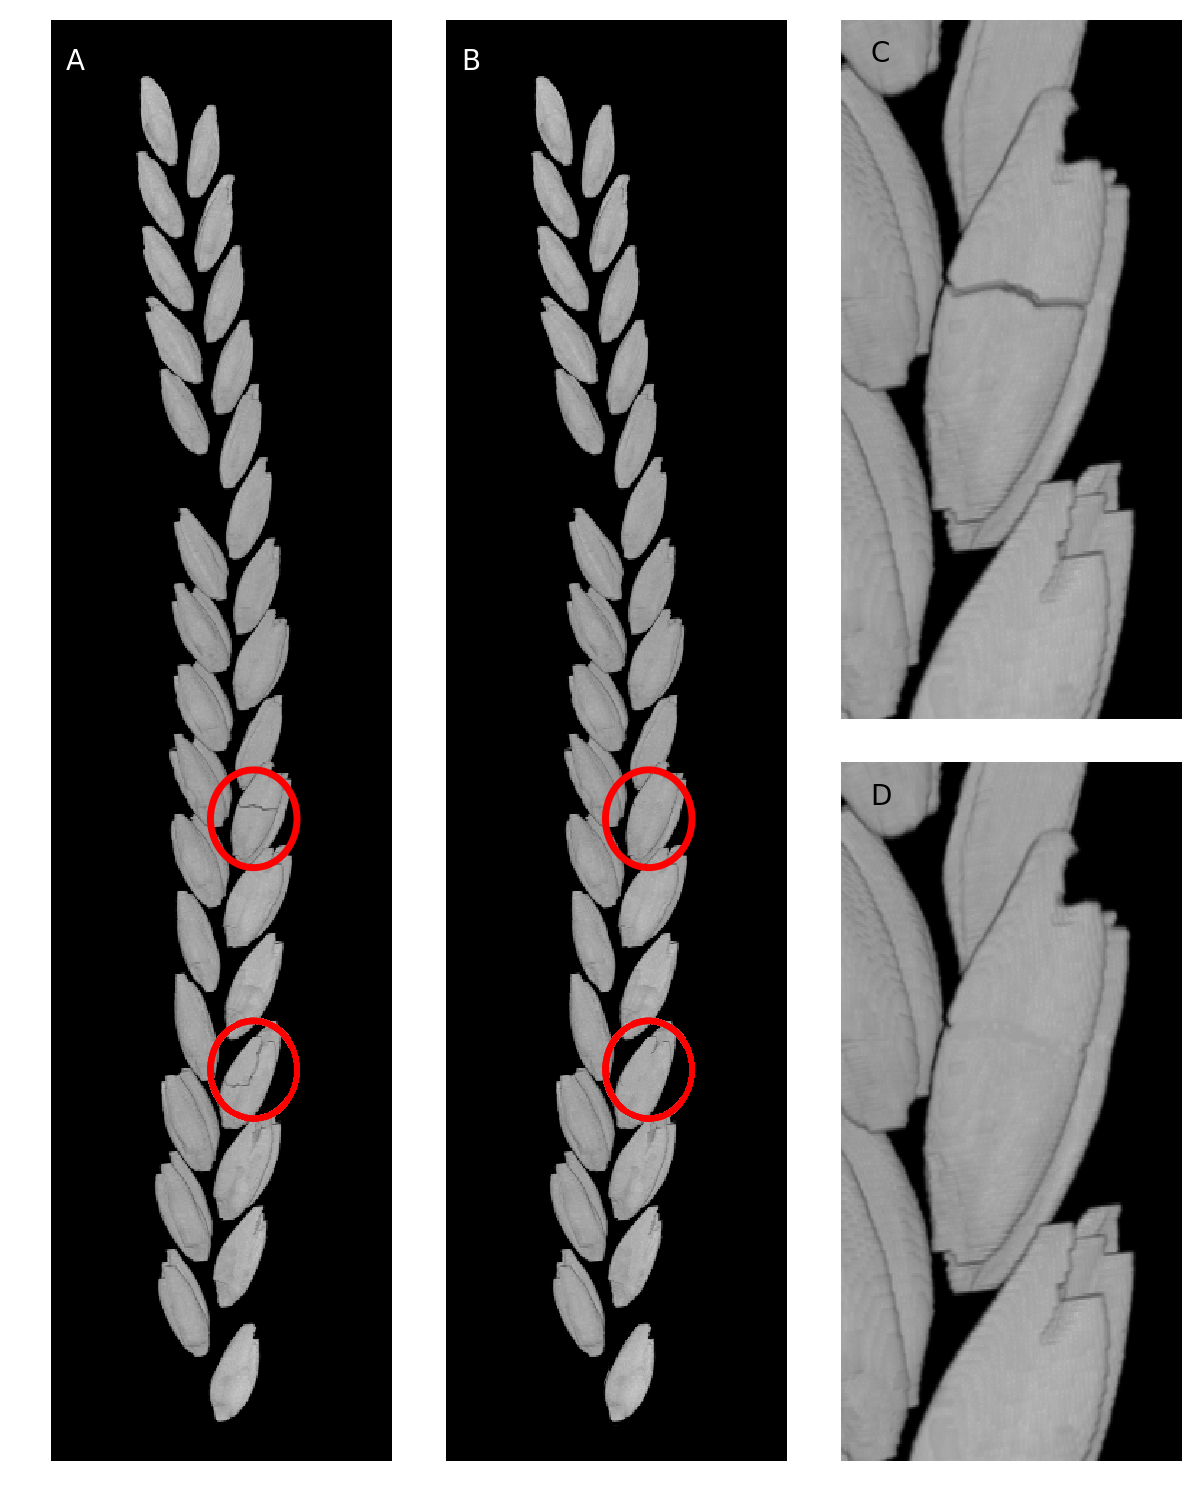
\includegraphics[width=14cm]{./images/watershedfigure.png}
\caption{\label{fig:org56eafe0}
\emph{A} showing before the new method, \emph{B} after, \emph{C} zoomed before, \emph{D} zoomed after.}
\end{figure}

\clearpage
\section{CT Analysing Library Methods}
\label{sec:orgc496d19}
The CT Analysing Library provided by this project, aims to reduce the amount of work and time required to organise, analyse and pull meaning out of \textmu{}-CT data.
Here several of the more novel features of the library are explained.

\subsection{CT Data Object}
\label{sec:org598ea5e}

The CT Analysing Library uses a mixture of object orientated (OOP) and functional programming paradigms, the main initialisation function for the object \emph{CTData} enables the storing of data and application of functions upon it, making data organisation much more straightforward.

\begin{listing}[htbp]
\begin{minted}[linenos,firstnumber=1,frame=lines,linenos=true,fontfamily=DejaVuSans]{python}
class CTData():
    def __init__(self, folder, rachis):
        """
        This is the initialise function for the CTData object,
        this will only need called once.

        @param folder the folder to look for data in
        @param rachis a boolean to decide to load in rachis data or not
        """
        try:
            self.make_dataframe(folder, get_rachis=rachis)
            self.clean_data()
            self.create_dimensions_ratio()
            self.df = self.df.reset_index(drop=True)
        except (ValueError, NoDataFoundException):
            raise NoDataFoundException
        self.additional_data = None
\end{minted}
\caption{\label{org20e137f}
CT Data Object Initialisation Method}
\end{listing}

\clearpage
\subsection{Loading Data}
\label{sec:org3dcdc76}

Initial data loading is performed by the \emph{gather\_data} function, it takes a folder string and performs a regular expression check for all CSV files. From the files found in this search this function performs separation of rachis information (data about the spike's inner nodes) and the files containing seed/grain data.

These are returned together as a tuple, the data found is stored as part of the \emph{CTData} object for use in the processing pipeline.

\begin{listing}[htbp]
\begin{minted}[linenos,firstnumber=1,frame=lines,linenos=true,fontfamily=DejaVuSans]{python}
def gather_data(self, folder):
    """
    this function gathers together all
    the data of interest

    @param folder is a starting folder
    @returns tuple of (seed files, rachis files)
    """

    # check the end of the folder has a '/'
    if folder[-1] != '/':
        folder = folder + '/'

    search_params = '{0}*/*.csv'
    candidate_files = glob(search_params.format(folder))

    # Check data was found
    if len(candidate_files) == 0:
        raise NoDataFoundException

    # we aren't bothered about the raw files so lets remove them
    candidate_files = [f for f in candidate_files if 'raw' not in f]

    # now let's separate out the rachis
    rachis = [f for f in candidate_files if 'rachis' in f]

    # and just assume the rest is what we want
    candidate_files = [f for f in candidate_files if 'rachis' not in f]

    return (candidate_files, rachis)
\end{minted}
\caption{\label{org77348df}
Loading Data Function}
\end{listing}

\clearpage
\subsection{Adding Spike Experiment Information}
\label{sec:org1be6507}

Using a loosely defined Microsoft excel (.xlsx) file, a file of additional information can be loaded into the \emph{CTData} object. This new information can be any information which is relevant to the individual scans.

This function \emph{get\_spike\_info} works by finding the matching column to join data on, then using the provided excel file it adds these new columns of information into the \emph{CTData} object.

By using \(\lambda\) functions (named \emph{look\_up} and \emph{gather\_data}) rapid allocation of information can be done in sections, applying hundreds of data entries to the existing data. This is one of many elements in this project which solves challenges in a very functional programming manner.

\begin{listing}[htbp]
\begin{minted}[linenos,firstnumber=1,frame=lines,linenos=true,fontfamily=DejaVuSans]{python}
def get_spike_info(df, excel_file, join_column='Folder#'):
    """
    This function should do something akin to adding additional
    information to the data frame

    @note there is some confusion in the NPPC about whether to use
    folder name or file name as the unique id when this is made into
    end-user software, a toggle should be added to allow this

    @param excel_file a file to attach and read data from
    @param join_column if the column for joining data is required
    """
    # Grab the linking excel file
    info = pd.read_excel(excel_file,
                         index_col='Folder#')
    # These are the features to grab
    features = list(info.columns)
    # Lambda to look up the feature in excel spreadsheet
    def look_up(x, y): return info.loc[x['folderid']][y]
    # Lambda form a series (data row) and apply it to dataframe
    def gather_data(x): return pd.Series([look_up(x, y) for y in features])
    df[features] = df.apply(gather_data, axis=1)
    # Return the copy
    return df
\end{minted}
\caption{\label{orgf059726}
Spike Information Joining Algorithm}
\end{listing}

\clearpage
\subsection{Spike Rejoining}
\label{sec:orgbb100ca}
The \emph{Scanco} \textmu{}-CT100 scanner (\emph{Scanco} Medical, Switzerland) allows for a carousel loading of samples, the maximum allowed length of a sample is \textasciitilde{}10cm, in this study the majority of wheat spikes exceed this limit. A solution was found in splitting these samples in half and creating two separated \textmu{}-CT scans.

This process means that post imaging these sample data need to be reconnected and the \(z\) axis of all scans need adjusted.

One of the main issues of this task is that there are multiple ways that rejoining could be implemented, this library provides a function that standardises the process. Making repeatable results much easier to produce.

The implementation for this searches through the provided data frame for spikes which are not marked as being 'all', that is to say complete and non-split. From these spikes left, they are either marked 'top' or 'bottom', using an associated 'Sample name' these can be linked. Once linked the top of the spikes need to have their \(z\) attribute increased by the size of the bottom spike.

\begin{listing}[htbp]
\begin{minted}[linenos,firstnumber=1,frame=lines,linenos=true,fontfamily=DejaVuSans]{python}
def join_spikes_by_rachis(self):
    """
    Important part of this function is that we accept that the data is what it is
    that is to say: rtop, rbot and Z are all orientated in the proper direction
    It's main purpose is to join split spikes by rachis nodes identified in the
    analysis process

    @param grain_df is the grain dataframe to take on-board
    """
    # So we are only really interested in grains which are not labelled with
    # 'all' in partition, so let's id them to start with
    for sn in self.df[self.df['Ear'] != 'all']['Sample name'].unique():

        # Calculate estimated bottom location of a spike
        bot = self.df.loc[(self.df['Sample name'] == sn)
                          & (self.df['Ear'] == 'bot')]['rbot']

        # Apply bottom measurement where required by incrementing
        # 'z' values to top scans
        self.df.loc[
            (self.df['Sample name'] == sn) &
            (self.df['Ear'] == 'top'), 'z'] =
                    self.df.loc[(self.df['Sample name'] == sn) &
                    (self.df['Ear'] == 'top'), 'z'] + bot
\end{minted}
\caption{\label{orgdf1c882}
Spike Rejoining Function}
\end{listing}

\clearpage
\subsection{Data Aggregating}
\label{sec:org70c385b}
The analysis method used is focused on extracting data on a per-grain basis, grains have a many to one relationship of spikes.

In order to look at the data on a spike-per-spike basis rather than from seed-to-seed the data needs to aggregated.

The function \emph{aggregate\_spike\_averages} takes a list of attributes to be aggregated and a manner of grouping the data. Using this data new columns are created based on median; mean; standard deviation; sum. These new columns are stored in the \emph{CTData} object directly.

\begin{listing}[htbp]
\begin{minted}[linenos,firstnumber=1,frame=lines,linenos=true,fontfamily=DejaVuSans]{python}
def aggregate_spike_averages(self, attributes, groupby):
    """
    This will aggregate features (specified by attributes) into their medians
    on a per-spike basis.

    Makes direct changes to the dataframe (self.df)

    @param attributes list of features to average
    @param groupby how the data should be aggregated
    """

    # Functions which are used as an apply to the dataframe
    trans_funcs = {'median': np.median,
                   'mean': np.mean, 'std': np.std, 'sum': np.sum}

    # For each attribute apply
    for att in attributes:

        # For each function apply to each attribute in turn
        for col, func in trans_funcs.items():

            # Add straight to the dataframe using appropriate formatting to keep
            # naming straightforward
            self.df['{0}_{1}'.format(col, att)] = self.df.groupby(groupby)[
                att].transform(func)

    # Also add some information on the counts of seeds per plant
    self.df['grain_count'] = self.df.groupby(
        groupby)[groupby].transform(len)
\end{minted}
\caption{\label{org6f251f9}
Aggregating Data Function}
\end{listing}

\clearpage
\subsection{Cleaning and Removing Erroneous Data}
\label{sec:orge5e6542}

Data are cleaned by calculating percentiles of minimum data, these extreme values are removed. In addition to this, values found in seed/grain literature are used to remove data based on known extremes \cite{Gegas2010,Hughes2017}.

\begin{listing}[htbp]
\begin{minted}[linenos,firstnumber=1,frame=lines,linenos=true,fontfamily=DejaVuSans]{python}
def clean_data(self, remove_small=False, remove_large=False):
    """
    Following parameters outlined in the
    CT software documentation I remove outliers
    which are known to be errors

    @param remove_small a boolean to remove small grains or not
    @param remove_large a boolean to remove larger grains or not
    """
    # Remove all data which has any null or none types
    self.df = self.df.dropna(axis=1, how='all')

    # Remove obviously wrong and too large grains
    self.df = self.df[self.df['surface_area'] < 100]
    self.df = self.df[self.df['volume'] > 3.50]  # this is given for brachy
    self.df = self.df[self.df['volume'] < 60]

    # If the large parameter is set then remove the upper 5th percentile of volume
    if remove_large:
        self.df = self.df[self.df['volume'] <
                          self.df['volume'].quantile(.95)]
    # If the large parameter is set then remove the lower 5th percentile of volume
    if remove_small:
        self.df = self.df[self.df['volume'] >
                          self.df['volume'].quantile(.05)]

\end{minted}
\caption{\label{orgad07663}
Cleaning Data}
\end{listing}

\clearpage
\subsection{Data Transformations (PCA)}
\label{sec:org260b48d}
In this project several data transformation algorithms are implemented uses the \emph{Scipy} library \cite{Oliphant2007}.

For principal component analysis (PCA), the CT Analysis Library implements it using two principal components (PCs) only. The decision to limit this library
to using only two PCs was made to keep data as easy to interpret as possible. Additionally experimentation with this transform shows a high percentage of
coverage and data explanation from only two PCs.

Prior to using the PC function, data are standardised, this is either done through log transforms or by Box Cox power transforms. This provides more normal data and allows for information to be more likely to provide a significant output.

\begin{listing}[htbp]
\begin{minted}[linenos,firstnumber=1,frame=lines,linenos=true,fontfamily=DejaVuSans]{python}
def perform_pca(df, features, groupby, groupby2=None,
                groupby3=None, standardise=False):
    """
    This function will perform a PCA and return the principle components as a
    dataframe.

    @param n_components components to check form
    @param df dataframe of the data to analyse
    @param features features from the dataframe to use
    @param groupby the column in the df to use
    @param standardise=False asks whether to standardise the data prior to PCA
    @returns a dataframe of the data, the pca object & the scaled data for reference
    """
    # Only use 2 pcs
    pca = PCA(components=2)
    # Standardise the data if requested
    data = standarise_data(
        df, features, groupby) if standardise else df.loc[:, features].values
    # Perform pca fitting on the chosen data
    principalComponents = pca.fit_transform(data)
    # form the pca into a dataframe with pca1 and 2 labelled
    principalDf = pd.DataFrame(data=principalComponents, columns=[
                               'principal component 1', 'principal component 2'])
    # Decide how to group the data into the final pca table to return
    # three options are given as multiple analysis may be required
    if groupby2 is None:
        return (pd.concat([principalDf, df[[groupby]]],
                          axis=1), pca, data)
    if groupby3 is None:
        return (pd.concat([principalDf, df[[groupby]],
                           df[[groupby2]]], axis=1), pca, data)
    else:
        return (pd.concat([principalDf, df[[groupby]],
                           df[[groupby2]], df[[groupby3]]], axis=1), pca, data)
\end{minted}
\caption{\label{orge55a0ff}
PCA Data Transform}
\end{listing}

\clearpage
\subsection{Bayesian Hypothesis Testing}
\label{sec:orgf2405ff}

Null-hypothesis significance testing (NHST) is done typically through T-test like functions, where the means of two groups are tested.
As a novel addition, this library provides an improvement upon NHST by using a Bayesian approach proposed by Kruschke in 2012 \cite{Kruschke2012}.

Here a full model is produced where data are first normalised through log transforms, model parameters set and then 1000 simulations ran via Markov chain Monte Carlo to produce a larger data sample to perform mean testing on.

The 1000 simulations are ran twice, these form two independent chains, checking of convergence and agreement on these random chains is performed to reduce the chance of error.

This function returns a \emph{trace} object which contains all of the data generated, the data of particular interest is the "difference of means" that this method calculates and the credible interval graphs which it returns the values for, figure:\ref{fig:org5fb2891} provides an example of such. The example provided shows the likelihood of two means of an interaction term of
\(length \times  depth \times width\) overlapping.

\begin{figure}[htbp]
\centering
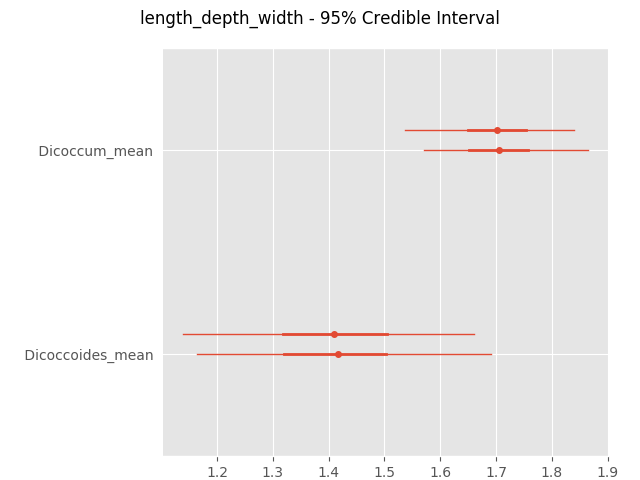
\includegraphics[width=15cm]{./images/ci.png}
\caption{\label{fig:org5fb2891}
An example credible interval produced by this method}
\end{figure}


The full model is explained later in this chapter in a much more informative manner and fully defined in terms of relevance to results of this project. Listing:\ref{org995f521} provides the python model implemented.

\begin{listing}[htbp]
\begin{minted}[linenos,firstnumber=1,frame=lines,linenos=true,fontfamily=DejaVuSans]{python}
def baysian_hypothesis_test(group1, group2, group1_name, group2_name):
    """
    Implements and uses the hypothesis test outlined as a robust replacement
    for the t-test
    @param group1 a numpy array to test
    @param group2 a numpy array to test
    @param group1_name the name of the first group
    @param group2_name the name of the second group
    @returns a summary dataframe
    """
    group1 = np.log10(group1)
    group2 = np.log10(group2)
    y = pd.DataFrame(dict(value=np.r_[group1, group2], group=np.r_[
                     [group1_name]*len(group1), [group2_name]*len(group2)]))
    mu_m = y.value.mean()
    mu_s = y.value.std()*2
    with pm.Model() as model:
        group1_mean = pm.Normal('{0}_mean'.format(group1_name), mu_m, sd=mu_s)
        group2_mean = pm.Normal('{0}_mean'.format(group2_name), mu_m, sd=mu_s)
    sig_low = 1
    sig_high = 1000
    with model:
        group1_std = pm.Uniform('{0}_std'.format(
            group1_name), lower=sig_low, upper=sig_high)
        group2_std = pm.Uniform('{0}_std'.format(
            group2_name), lower=sig_low, upper=sig_high)

    with model:
        nu = pm.Exponential('nu_minus_one', 1/29.) + 1
    with model:
        lambda_1 = group1_std**-2
        lambda_2 = group2_std**-2
        group1 = pm.StudentT(group1_name, nu=nu, mu=group1_mean,
                             lam=lambda_1, observed=group1)
        group2 = pm.StudentT(group2_name, nu=nu, mu=group2_mean,
                             lam=lambda_2, observed=group2)
    with model:
        diff_of_means = pm.Deterministic(
            'difference of means', group1_mean - group2_mean)
        diff_of_stds = pm.Deterministic(
            'difference of stds', group1_std - group2_std)
        effect_size = pm.Deterministic('effect size',
                                       diff_of_means /np.sqrt((group1_std**2 +
                                       group2_std**2) / 2))
    with model:
        trace = pm.sample(2000, cores=2)
        return trace, pm.summary(trace, varnames=['difference of means',
                                                  'difference of stds','effect size'])
\end{minted}
\caption{\label{org995f521}
Bayesian Model Function}
\end{listing}


\clearpage


\section{CT GUI Application Methods}
\label{sec:org48765c6}
The CT GUI Application enables a researcher to perform analysis with a high degree of automation and ease of use. Here several of the elements of software engineering behind this application and its design are explored.

\subsection{Windows}
\label{sec:org2d7de63}
The CT GUI Application uses a tabbed interface, each tab carries out a specific task. This follows Gestalt themes of making user interfaces inherently clear with grouping together functionality in specific areas.

\subsubsection{The Load Data Window}
\label{sec:org4de37cd}
This window acts as the opening to the software, where a user can select loading of files and data. As well as options such as whether to load spike rachis information.
\begin{figure}[htbp]
\centering
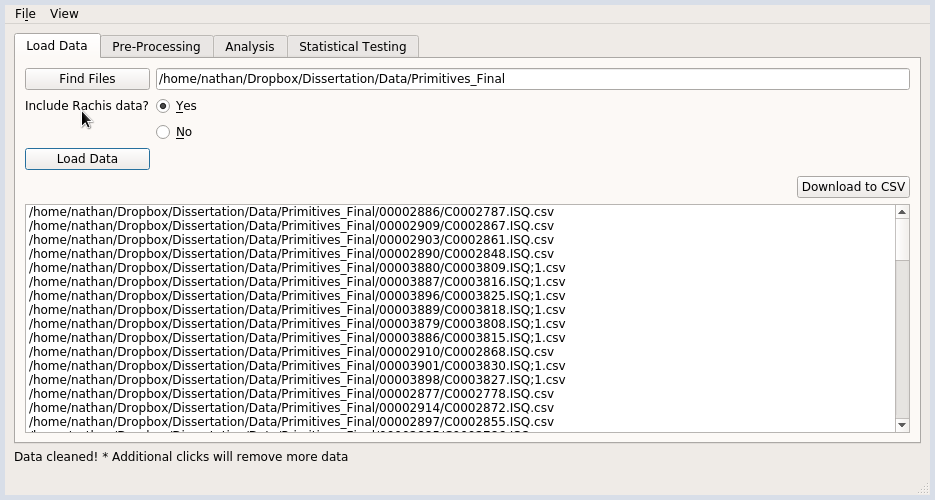
\includegraphics[width=11.5cm]{./images/Screenshots/clean_data_remove_large.png}
\caption{\label{fig:org16a5f21}
The Initial Data Loading Window for the GUI}
\end{figure}
\subsubsection{Table View}
\label{sec:orgadca926}
In addition to the tabs provide by the application, a table view is accessed via the system menu bar. This allows an alternative view of the data which is not pictorial.
\begin{figure}[htbp]
\centering
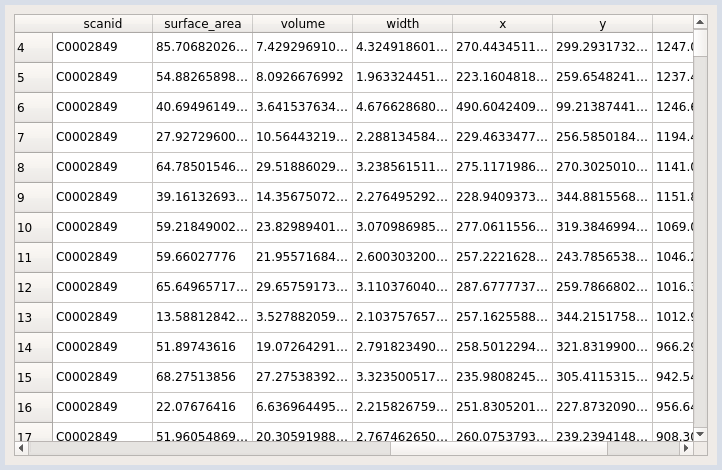
\includegraphics[width=5cm]{./images/table.png}
\caption{\label{fig:orgb03ce40}
The Table view in used in the GUI}
\end{figure}
\subsubsection{The Clean Data Window}
\label{sec:orgf01cae6}
The second tab this software introduces is a data cleaning and preparation window. This tab allows additional data to be loaded into an experiment such as scan names, genotype information etc. Options to clean the data by removing outliers is also presented with various options.
\begin{figure}[htbp]
\centering
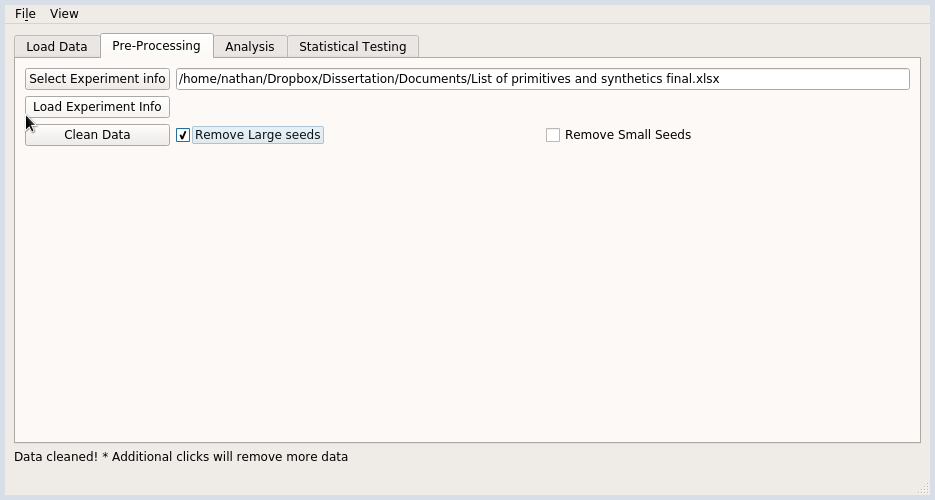
\includegraphics[width=11.5cm]{./images/clean.png}
\caption{\label{fig:org5070cda}
The Data Cleaning and Loading Window for the GUI}
\end{figure}

\subsubsection{The Analysis Window}
\label{sec:orgbaad1fe}
The third tab is made available once data has been loaded, access to it prior to loading data will cause the application to provide the user with a warning that it will not function correctly without loading information first.

This window gives a user the ability to rapidly investigate data, it enables the plotting of data via histograms and box plots, both of these are incredibly useful for initial investigation of data. It tells researchers a lot about the shape of their data and allows them to see an estimate of means, averages and spread of data.

\begin{figure}[htbp]
\centering
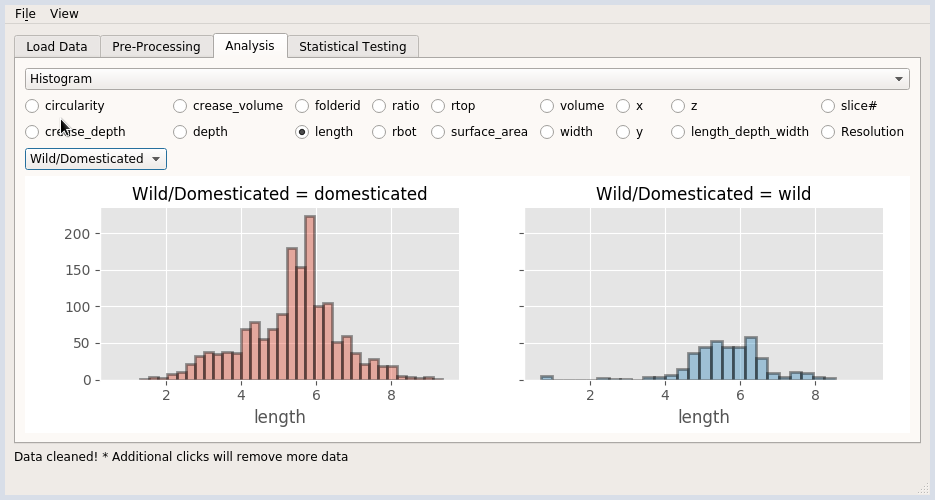
\includegraphics[width=11.5cm]{./images/analysiswindow.png}
\caption{\label{fig:orgbcbd211}
The Analysis/Investagation Window for the GUI}
\end{figure}

\subsubsection{The Hypothesis Testing Window}
\label{sec:orgf64c877}
The fourth and final window which this application presents is a method for performing hypothesis testing on the loaded data.

The method for implementing tests is flexible and more could be easily implemented; currently the Student's T-test, Welch's T-test and a Bayesian T-test are implemented to give a range of NHSTs.

\begin{figure}[htbp]
\centering
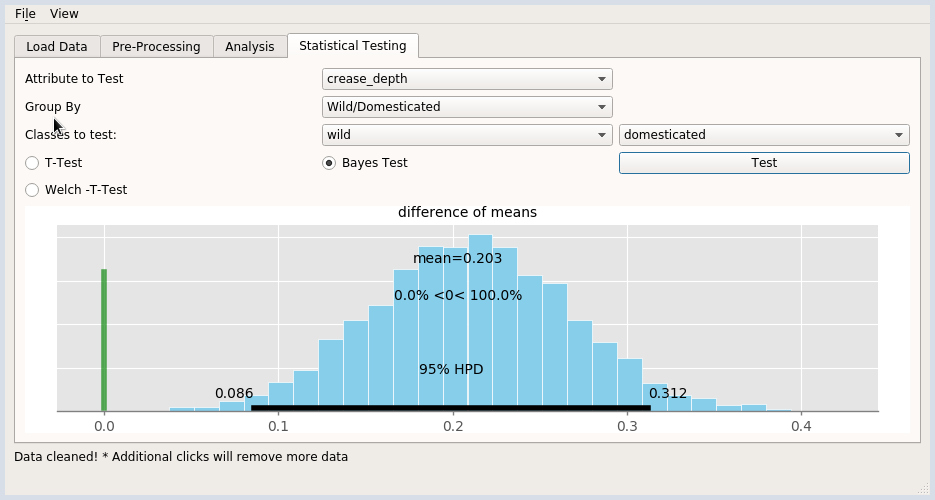
\includegraphics[width=11.5cm]{./images/differenceofmeanswindow.png}
\caption{\label{fig:org7f2def2}
The Hypothesis Testing Window for the GUI with a difference of means plot}
\end{figure}

\begin{figure}[htbp]
\centering
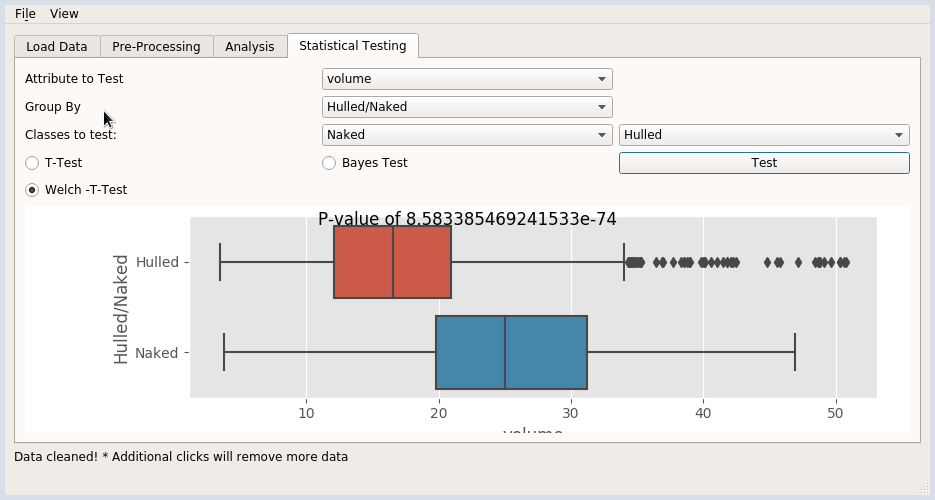
\includegraphics[width=11.5cm]{./images/pvaltest.png}
\caption{\label{fig:org903243d}
The Hypothesis Testing Window for the GUI with a T-test and boxplot}
\end{figure}

\clearpage
\subsection{QT GUI Loading}
\label{sec:orgc3a679b}

The GUI is started from a minimal main method, as dictated by standard model-view-controller (MVC) convention. This leads to an \emph{AppWindow} object which inherits from the \emph{Qt}'s library \emph{QMainWindow}. The MVC model comes into full effect in the constructor for this class.

This constructor assigns a \emph{PyQt5} GUI file to itself. This allows for a predefined series of objects with rigid layout to be used in the software.

A series of setup functions are called which connect triggers (functions called when GUI elements are interacted with) to the correct controllers.

This main window spawns and hosts the controllers which dictate handling of their respective window (tab).


\begin{listing}[htbp]
\begin{minted}[linenos,firstnumber=1,frame=lines,linenos=true,fontfamily=DejaVuSans]{python}
class AppWindow(QMainWindow):
    def __init__(self):
        super().__init__()
        self.ui = Ui_MainWindow()
        self.ui.setupUi(self)
        self.setup_menu_functions()

        # Load in Controllers
        self.find_files_controller = FindFilesWindow(self, self.ui)
        self.analysis_controller = AnalysisWindow(self, self.ui)
        self.ui.master_tab.currentChanged.connect(self.update_analysis_view)
        self.pre_process_controller = PreProcessWindow(self, self.ui)
        self.stats_test_controller = StatsTestWindow(self, self.ui)

        # Set GUI icon for beautification
        self.setWindowIcon(QtGui.QIcon('./images/logo.png'))

        # init some variables
        # Words cannot describe the importance of this object
        self.data = None

        # init states
        self.setup_default_states()
        self.show()
\end{minted}
\caption{\label{org362567d}
The AppWindow Class' initialisation function}
\end{listing}

\clearpage

\subsection{Connecting Signals from GUI to Function Calls}
\label{sec:org499f582}
In example:\ref{orgc08b216} lines 11,12,13 show how the UI object has individual members, each of these has a "clicked" trigger, which when triggered calls a function pointer which this controller handles.
\begin{listing}[htbp]
\begin{minted}[frame=lines,linenos=true,fontfamily=DejaVuSans]{python}
class FindFilesWindow():
    def __init__(self, window, ui):
        self.ui = ui
        self.window = window
        self.connect_view_functions()
    def connect_view_functions(self):
        # Load data page
        self.ui.btn_find_files.clicked.connect(self.search_for_files)
        self.ui.btn_load_data.clicked.connect(self.find_files)
        self.ui.btn_to_csv.clicked.connect(self.save_file_dialog)
\end{minted}
\caption{\label{orgc08b216}
Example of connecting function pointers}
\end{listing}

\subsection{Integration with CT Analysis Library}
\label{sec:org96329f2}

The integration with the CT Analysis Library is frequent and spread throughout this application and functions as a key dependency for data organisation.

One example of this is in the load data function shown in example:\ref{org36b57d4}. Here the custom exception classes are imported and used for data already loaded, as well as the loading functions itself.

\begin{listing}[htbp]
\begin{minted}[linenos,firstnumber=1,frame=lines,linenos=true,fontfamily=DejaVuSans]{python}
def find_files(self):
    try:
        if self.window.get_data() is not None:
            raise DataAlreadyLoaded
        self.window.set_data(CTGUIData(self.ui.directory.text(),
                                       self.ui.rdb_rachis_yes.isChecked()))
        if self.window.get_data():
            self.ui.btn_to_csv.setEnabled(True)
            self.ui.tab_preprocess.setEnabled(True)
            self.ui.tab_analysis.setEnabled(True)
            self.set_files_list()
            self.ui.lbl_status.setText('Data loaded!')
    except TypeError as e:
        QMessageBox.warning(self.window, "Finding Files Error",
                            "Couldn't find files in given location")
    except DataAlreadyLoaded as e:
        QMessageBox.warning(self.window, "Data Already Loaded",
                            "Sorry! You've already loaded in data")
\end{minted}
\caption{\label{org36b57d4}
The load data function from the load\_data window}
\end{listing}
\subsection{Plot Window Rendering}
\label{sec:orgfae34d6}

Plots where rendered in this application by creating a custom object which inherited from the \emph{matplotlib} backend \emph{qt5agg}. This object is both a \emph{Qt} widget and a \emph{matplotlib} figure. This class provided a straightforward mechanism that would allow for any style of plot (which \emph{matplotlib} supports) to be created.

This object also acts as a template class for actual implementations, each window type of this application that uses plots (\emph{Analysis Tab}; \emph{Hypothesis Testing Tab}) creates a custom \emph{MyMplCanvas} child class. To specifically handle inputs which are unique to that window.

The unique inheritance of this class allows it to be treated as a \emph{Qt} widget, when it is created by a controller it  can be added to the view with no alterations required.

\begin{listing}[htbp]
\begin{minted}[frame=lines,linenos=true,fontfamily=DejaVuSans]{python}
from matplotlib.backends.backend_qt5agg import FigureCanvasQTAgg as FigureCanvas
...
  class MyMplCanvas(FigureCanvas):
      """Ultimately, this is a QWidget (as well as a FigureCanvasAgg, etc.)."""

      def __init__(self, parent=None, window=None, df=None,
                   column=None, width=5, height=4,
                   dpi=100, plot_type=None, group_by=None, ttest=False):

          if group_by == 'None':
              self.group_by = None
          else:
              self.group_by = group_by
          self.ttest = ttest
          self.window = window
          self.plot_type = plot_type
          self.column = column

          if plot_type == 'histogram' and self.group_by is not None:
              self.fig = self.facet_hist(df, column, group_by)
              FigureCanvas.__init__(self, self.fig)
          else:
              self.fig = Figure(figsize=(width, height), dpi=dpi)
              self.axes = self.fig.add_subplot(111)
              FigureCanvas.__init__(self, self.fig)
              self.compute_initial_figure(self.axes, df)

          self.setParent(parent)
          FigureCanvas.setSizePolicy(self,
                                     QtWidgets.QSizePolicy.Expanding,
                                     QtWidgets.QSizePolicy.Expanding)
          FigureCanvas.updateGeometry(self)
\end{minted}
\caption{\label{orgf1895f8}
The Matplotlib FigureCanvas Polymorphic Class}
\end{listing}

\subsection{Creating GUI Elements When Required}
\label{sec:org317a1b5}

One of the key features of this project, and this GUI application specifically is the ability to handle dynamic input. The loading additional experiment information allows for the opportunity for never-before seen data to be presented. This allows users to define custom classification and testing groups. An example from the research element of this project is shown in figure:\ref{fig:orgbe7fc79}.

\begin{figure}[htbp]
\centering
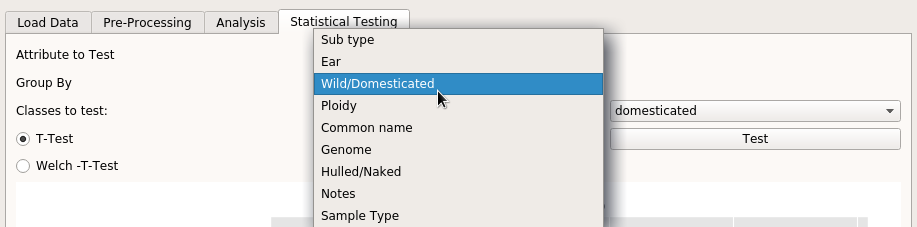
\includegraphics[width=10cm]{./images/dynamicselection.png}
\caption{\label{fig:orgbe7fc79}
Showing how groups are loaded from columns for potential data splitting and testing}
\end{figure}

Here in example:\ref{org13e2c0d} lines 16,17 show that combo buttons are created for the \emph{Hypothesis Testing} window to display to a user. A similar system is added for the \emph{Analysis Window} where decisions are carried out as to what columns could be potentially used for object grouping. This is calculated by dividing the columns contents, if it is numeric and has repeating elements or if the contents are text then they are (generally) applicable for use in grouping grains for testing or plotting.

\begin{listing}[htbp]
\begin{minted}[frame=lines,linenos=true,fontfamily=DejaVuSans]{python}
class TestWindowView():
    def __init__(self,df,ui,plot_type):
        """
        Given a dataframe and a layout spec
        this class populates appropriate radio button functionality
        """
        self.df = df
        self.ui = ui
        self.plot_type = plot_type
        self.ui.cb_test_grouping.clear()
        self.ui.cb_test_attribute.clear()
        # Line up attributes
        self.ui.cb_test_attribute.addItems(list(
            filter(lambda x: is_numeric_dtype(df[x]), df.columns)))

        # Find groups
        self.ui.cb_test_grouping.addItems(
            self.find_candidates_for_grouping(self.df))

    def find_candidates_for_grouping(self, df):
        lst = []
        for c in df.columns:
            if len(df[c].unique()) < 30:
                if not is_numeric_dtype(df[c]):
                    lst.append(c)
        return lst
\end{minted}
\caption{\label{org13e2c0d}
The Hypothesis Testing Window class}
\end{listing}

\subsection{Dynamically Generating Plots}
\label{sec:orga768ce7}
This application provides the ability to make plots instantly, without requiring input from the user to refresh or reload a window.

To do this, the existing canvas window is repainted based on parameter input. Example:\ref{orgf9c8736}
shows how this is implemented. A series of conditionals based on UI elements provides data about what data to use and type of plot to use also.

When a hypothesis test is being carried out, this function will call the \emph{CTData} library to perform the test and return a P-value which is then applied to the plot's title.

\begin{listing}[htbp]
\begin{minted}[frame=lines,linenos=true,fontfamily=DejaVuSans]{python}
def compute_initial_figure(self, axes, df):
    try:
        if self.plot_type == 'histogram':
            sns.distplot(df[self.column], ax=self.axes,
                         kde=False, hist_kws=dict(edgecolor="k", linewidth=2))
        elif self.plot_type == 'boxplot' or self.plot_type == 'welch':
            sns.boxplot(data=df, x=self.column,
                        y=self.group_by, ax=self.axes)
            if self.ttest:
                u = list(df[self.group_by].unique())
                s1 = df[df[self.group_by] == u[0]][self.column]
                try:
                    s2 = df[df[self.group_by] == u[1]][self.column]
                except IndexError:
                    s2 = s1
                if self.plot_type == 'welch':
                    p = perform_t_test(s1, s2, equal_var=False)
                else:
                    p = perform_t_test(s1, s2)
                self.fig.suptitle('P-value of {0}'.format(p))
            elif self.plot_type == 'bayes':
                u = list(df[self.group_by].unique())
                s1 = np.array(df[df[self.group_by] == u[0]][self.column])
                try:
                    s2 = np.array(df[df[self.group_by] == u[1]][self.column])
                    trace, x = baysian_hypothesis_test(s1, s2, u[0], u[1])
                    plot_difference_of_means(trace, ax=self.axes)
\end{minted}
\caption{\label{orgf9c8736}
Example code of how figures are computed and implemented using \emph{Seaborn} and \emph{Matplotlib}}
\end{listing}

\clearpage
\subsection{Creating Facet Plots}
\label{sec:org30f7d5a}

To compare data in more than a single dimension the \emph{FacetFrid} function from the \emph{Seaborn} library is used. This provides a simple method of creating multiple plots in a single figure.

An example of this is shown when dividing data by ploidy and comparing distributions via histograms in figure:\ref{fig:orgb6a9721}.

\begin{figure}[htbp]
\centering
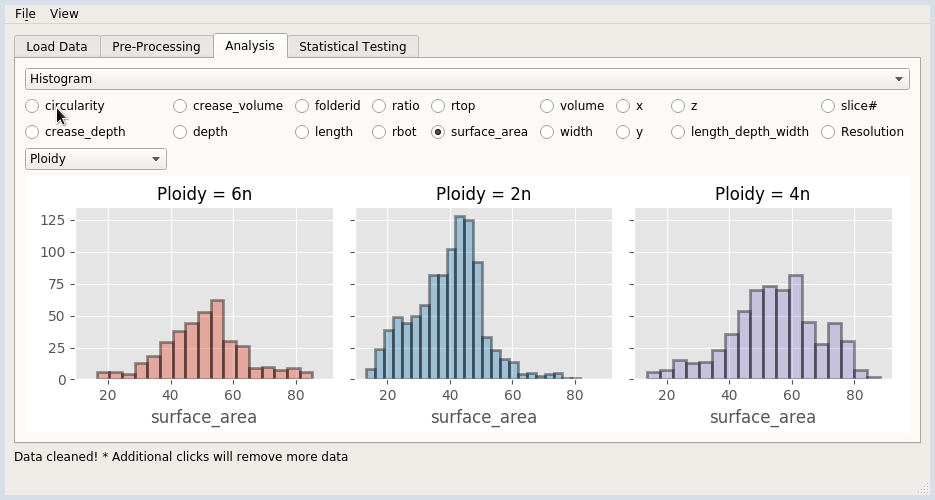
\includegraphics[width=12cm]{./images/facet_example.png}
\caption{\label{fig:orgb6a9721}
Example of facet plotting by ploidy by grain surface area}
\end{figure}

The implementation of \emph{facet plots} would be simple, however the ability to create sensible plots that organise into a well spaced grid requires additional input.

Example:\ref{org7f01c57} shows on lines 3,5,7 how decisions are made to best arrange the grid. Decisions are made based on the unique number of columns a grouping variable provides. As well this,  additional arguments are  used to indicate further aesthetics of the plots.

\begin{listing}[htbp]
\begin{minted}[frame=lines,linenos=true,fontfamily=DejaVuSans]{python}
def facet_hist(self, df, column, group_by):
    col_wrap = len(df[group_by].unique()) // 2
    if col_wrap < 4:
        col_wrap = None
    g = sns.FacetGrid(df, hue=group_by, col=group_by,
                      col_wrap=col_wrap)
    g = g.map(sns.distplot, column, kde=False,
              hist_kws=dict(edgecolor="k", linewidth=2))
    g.fig.tight_layout()
    return g.fig
\end{minted}
\caption{\label{org7f01c57}
Using Facet wrapping to provide}
\end{listing}

\section{Data Analysis Methods}
\label{sec:orgb8367bb}
The research elements of this project went through two distinct phases; the first round of investigation made use of statistical methods most commonly used in similar fields of research. \emph{ANOVA}, Students T-Test and PCA have been heavily used and are well accepted in grain analysis studies \cite{Gegas2010,Hughes2017,Xie2015}.

Initial findings showed that a more complex model would be required in order to make the best use out of the scientific data which this study produced.

The data which had been gathered, being from such a wide range of samples meant that sample count was relatively low. Distributions of data would also indicate that there were missing elements, with such wide standard deviations.

The solution devised to solve these problems is a Bayesian based model. The choice of this model comes from Bayesian statistics being more and more frequent in biological studies \cite{Kruschke2012,Pullen2014}. Additionally, a major strength of Bayesian statistics is its ability to adapt to missing data points and make best use of data available.

\subsection{Bayesian Analysis Model}
\label{sec:orge3c98a0}

Douglas H. Johnson stated that "Despite their wide use in scientific journals \ldots{}, statistical  hypothesis tests add very little value to the products of research" \cite{Johnson1999a}. In order to answer more complex, more meaningful questions about biological data more detailed and informative approaches are needed, classical methods which involve "p-values" are felt to not be complete solutions \cite{Goodman1999}.

By moving towards an evidence based model with Bayesian statistics, it is possible to provide interpretable answers, such as “the true parameter \(\theta\) has a probability of 0.95 of falling in a 95\% credible interval.”

The model provided by this project is an interpretation of the Bayesian T-test proposed by Kruschke in 2012 \cite{Kruschke2012}.

\subsubsection{Bayes Theorem}
\label{sec:orgf87da98}

Modern Bayesian interpretations use the simplified model of Bayes original theorem, equation:\ref{eq:org04b0f96} is the basis of the implemented model in this project. This states that: the posterior is proportional to the likelihood times the prior.

\begin{align}
\label{eq:org04b0f96}
  &\begin{aligned}
  P(A|B) \propto P(B|A) \times P(A)
  \end{aligned}
\end{align}
\myequations{Bayesian Statement}


\subsection{Likelihood}
\label{sec:org9ecf6bd}
The likelihood is described by the Student's T-test. Where each group \(g\) to be tested presents element \(y_i\) to a percentage likelihood of fitting a distribution \(T\) .

 \begin{align}
\label{eq:orgaa8f721}
   &\begin{aligned}
y_i^{(g)} \sim T(\nu, \mu, \sigma)
   \end{aligned}
 \end{align}
\myequations{Likelihood of Model}

\subsubsection{\(\nu\) (Degrees of freedom)}
\label{sec:org246eaaa}
The degrees of freedom used is given as an exponential as described by
Krusche \cite{Kruschke2012}. This is represented as \(\nu = 30\).

 \begin{align}
\label{eq:orged47056}
   &\begin{aligned}
\nu = 30
   \end{aligned}
 \end{align}
\myequations{Degrees of freedom used in Bayesian model}

\begin{figure}[htbp]
\centering
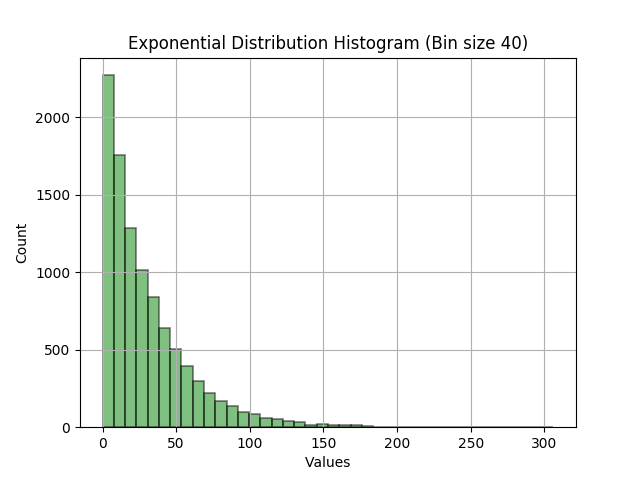
\includegraphics[width=7cm]{./images/dist2.png}
\caption{\label{fig:org2925053}
Exponential Distribution of 30}
\end{figure}

\subsubsection{\(\mu\) (Mean)}
\label{sec:org6cf8013}
This is assumed similar for groups \(g\). The data are real-values and normal priors are applied (to ensure the posterior is treated similarly).
Twice the standard deviation ensures no values are favoured in the model initially.

 \begin{align}
\label{eq:orge98fbcd}
   &\begin{aligned}
\mu_k \sim N(\bar{x},2s)
   \end{aligned}
 \end{align}
\myequations{Mean equation used in Bayesian model}

\begin{figure}[htbp]
\centering
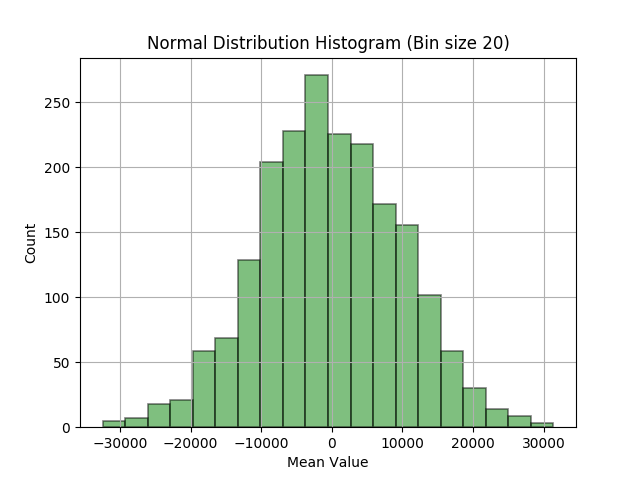
\includegraphics[width=7cm]{./images/mu.png}
\caption{\label{fig:org90ba37b}
Normal\((\bar{x},2s)\)}
\end{figure}


\subsubsection{\(\sigma\) (Standard Deviation)}
\label{sec:orge784012}
A large window for standard deviation is used (1,10000). Whilst no values in the model will have this range, it makes no difference due to random sampling via Markov chain Monte Carlo.

 \begin{align}
\label{eq:orgca61c38}
   &\begin{aligned}
\text{Uniform}(1,10000)
   \end{aligned}
 \end{align}
\myequations{Standard Deviation used in Bayesian model}


\begin{figure}[htbp]
\centering
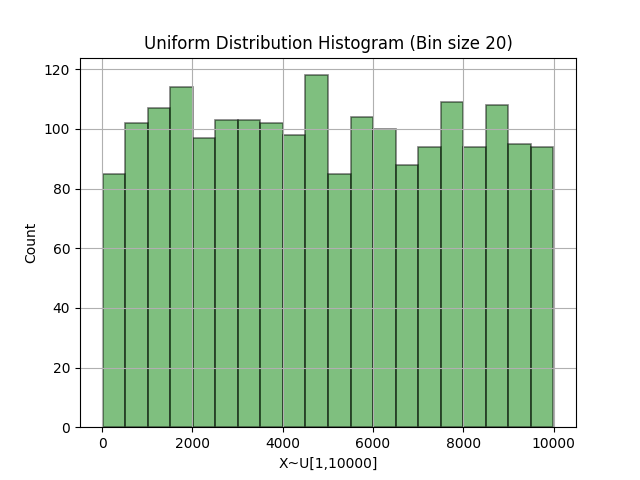
\includegraphics[width=7cm]{./images/dist.png}
\caption{\label{fig:orgd86d1b6}
Uniform(1,10000)}
\end{figure}


\subsection{Bayesian Hypothesis Testing Example}
\label{sec:org17db0ec}
A worked example is provided to demonstrate the power of this model.
\subsubsection{Input Data}
\label{sec:org6086ac9}
Given 20 data points of a simulated set of seed/grain lengths, it is generally not enough information to get a significant result from a T-Test. The data is sparse and not informative.

Figure:\ref{fig:org189a8a5} provides the simulated data in the form of a histogram where two groups, 'g1' and 'g2' have been used. These are considered the input for the model priors.
\begin{figure}[htbp]
\centering
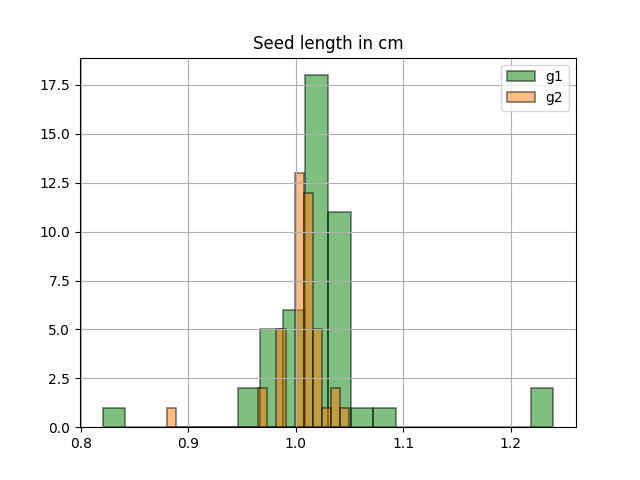
\includegraphics[width=7cm]{./images/exampledata.png}
\caption{\label{fig:org189a8a5}
Histogram of example input data}
\end{figure}

\subsubsection{Posterior Output}
\label{sec:org64eca83}
By applying the method outlined in code example:\ref{org995f521} and defined by equation:\ref{eq:orgaa8f721} the posterior predictions can generate 1000 random samples from the perceived distributions of the data. Based on the probability of each value existing within the priors' distribution.

Figure:\ref{fig:org564172a} demonstrates the expanded data set created by the posterior predictions.
\begin{figure}[htbp]
\centering
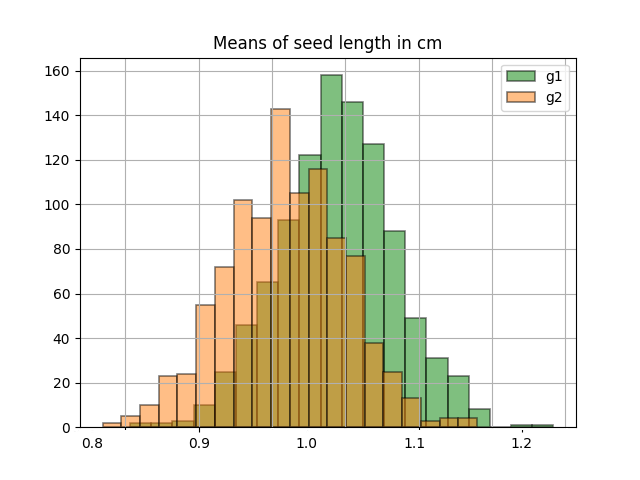
\includegraphics[width=7cm]{./images/examplebayes.png}
\caption{\label{fig:org564172a}
Histogram of example posterior data}
\end{figure}

\subsubsection{Difference of Means}
\label{sec:org9555e8b}
Using the created data, a simple \(\mu^1 - \mu^2\) will provide the difference of group 'g1' and group 'g2' means. Which can be used to interpret the significance likelihood of the groups having different means.

For the provided example data this model states that there is a 25.3\% chance that the two means of these groups are different. This is represented in figure:\ref{fig:org73534c8}.
\begin{figure}[htbp]
\centering
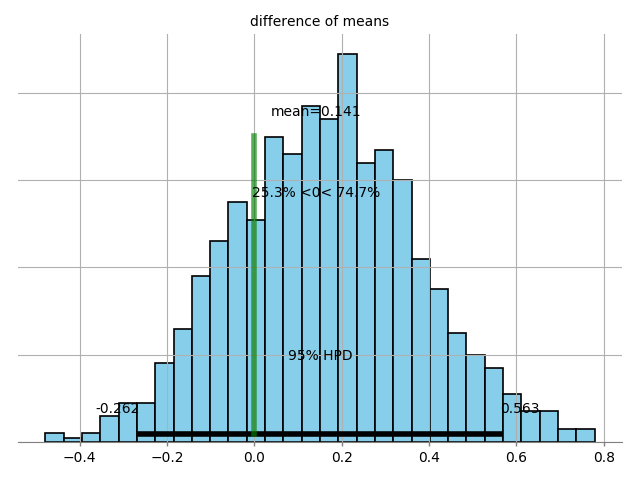
\includegraphics[width=7cm]{./images/examplebayes2.png}
\caption{\label{fig:org73534c8}
Difference of means plot - \(\mu^1 - \mu^2\)}
\end{figure}



\chapter{Results}
\label{sec:org0878180}
The research goals behind this project are focused on developing and modelling information on wheat domestication.

With statistical software created specifically to utilise \textmu{}-CT image data on wheat grains, five comparison groups were highlighted for investigation. Two main goals exist in these results, the chosen groupings aim to isolate both:

\begin{enumerate}
\item The Effects of ploidy on grain morphology
\item Domestication's influence on grain morphology
\end{enumerate}

Previous studies have used two dimensional morphometric analysis with flatbed scanning systems, Gegas et al. demonstrated through a \emph{Triticum} mapping population how these data could be used as a framework to partially explain variation in wheat \cite{Gegas2010}. This project expands by providing new phenotypes previously not examined.

\section{Bayesian Modelling}
\label{sec:orgcc7ca8f}
The designed Bayesian model previously described has been used as the basis for these results. Here a credible interval of 95\% of the data is presented. Null-hypothesis are tested against a difference of means. Data which present >99\% chance of different means are considered highly significant, >90\% is considered significant (similar to P<0.05 and P<0.01 is used).


\section{Grain Width is Not Affected by Domestication}
\label{sec:org4b024b3}

The groups \emph{T. beoticum} and \emph{T. monococcum} show (supplemental figure:\ref{fig:group1}) that width is significantly different, a 8.6\% chance that the mean of \emph{T. beoticum} width is greater than \emph{T. monococcum} is reported.

The reported change in width for tetraploids \emph{T. dicoccum} and \emph{T. dicoccoides} is not significant. A 36.3\% chance exists that the means of the groups are different, which is not a strong difference based on our model.

With one group agreeing to the null-hypothesis and one rejecting it, there is not enough evidence to fully reject that width is associated to solely domestication.

\clearpage
\section{Grain Length is Not Affected by Domestication}
\label{sec:org40b3787}

Here, this project has demonstrated that for the diploid genotypes \emph{T. beoticum} and \emph{T. monococcum} there is no significant difference in means. The provided model has predicted that there is a 49.6\% (figure:\ref{fig:lenmeansdiff}) that these two genotypes are different, this indicates a near perfect overlap of expected data.

\begin{figure}[!ht]
  \subfloat[\label{subfig-1:length}]{%
    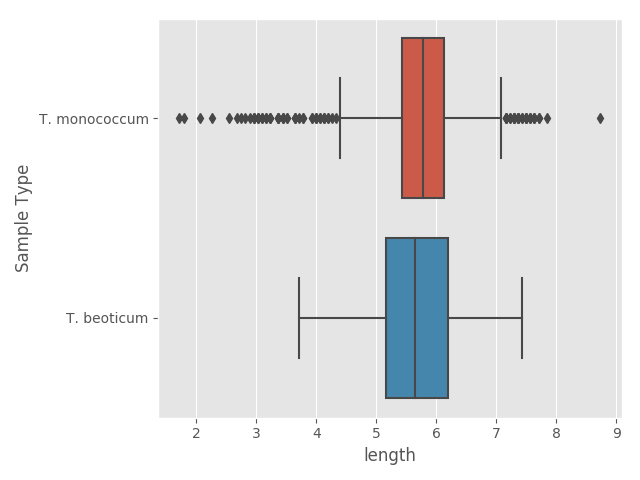
\includegraphics[width=0.45\textwidth]{./images/results/group1/length.png}
  }
  \hfill
  \subfloat[\label{subfig-2:Width}]{%
    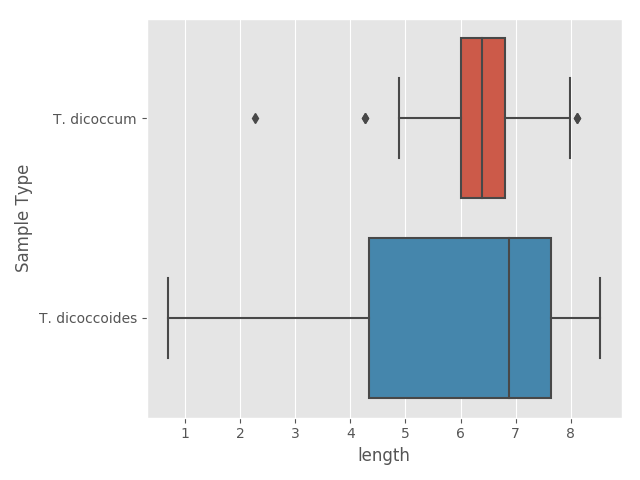
\includegraphics[width=0.45\textwidth]{./images/results/group2/length.png}
  }
  \caption{Boxplots for (a) diploid (2N) wild (red) and domesticated (blue) grains, (b) tetraploid (4N) wild (red) and domesticated (blue) grains}
  \label{fig:lendemest}
\end{figure}

For the tetraploid genotypes \emph{T. dicoccum} and \emph{T. dicoccoides} the effect of domestication appears statistically insignificant. A 27.3\% chance is reported as the likelihood of both means being independent. Whilst the data leans towards \emph{T. dicoccum} having a larger mean, there is insufficient evidence to reject that grain length is not effected by domestication.

Results from diploid and tetraploid genotypes, compared by domestication status, have shown no evidence to suggest that grain length is effected by domestication.


\begin{figure}[!ht]
  \subfloat[\label{subfig-1:length}]{%
    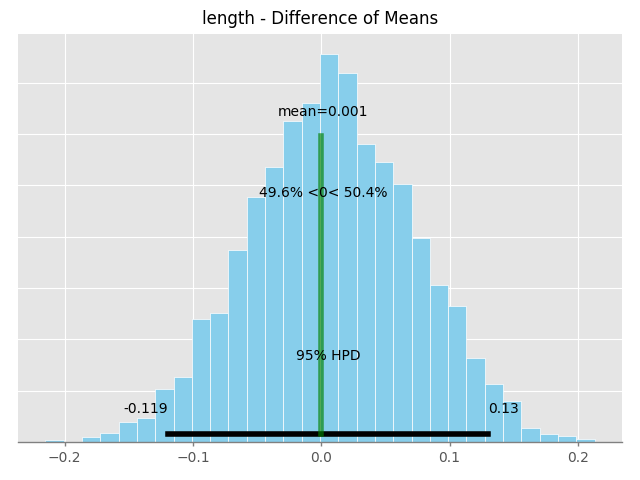
\includegraphics[width=0.45\textwidth]{./images/results/group1/bayes_difference_of_means_length.png}
  }
  \hfill
  \subfloat[\label{subfig-2:Width}]{%
    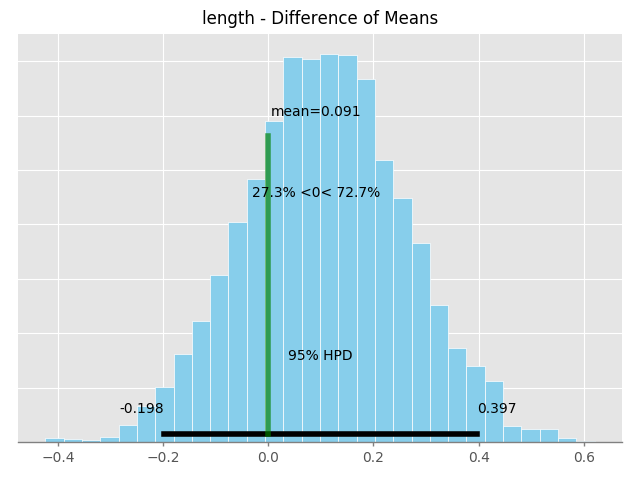
\includegraphics[width=0.45\textwidth]{./images/results/group2/bayes_difference_of_means_length.png}
  }
  \caption{Difference of means plots of wild and domesticated genotypes for length in (a) diploid (2N) grains,(b) tetraploid (4N) grains}
  \label{fig:lenmeansdiff}
\end{figure}
\clearpage

\section{Grain Volume Increases with Domestication}
\label{sec:org172e26b}

For volume, the diploid samples \emph{T. beoticum}, \emph{T. monococcum}  and the tetraploids \emph{T. dicoccum}  \emph{T. dicoccoides} when internally compared have shown that the difference in domestication is highly significant.

\begin{figure}[!ht]
  \subfloat[\label{subfig-1:length}]{%
    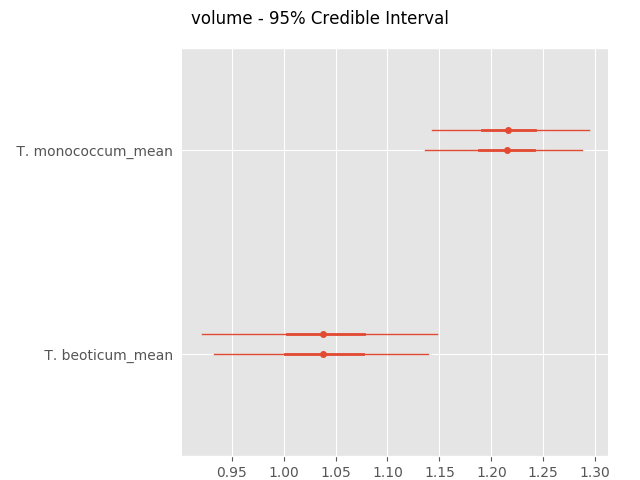
\includegraphics[width=0.45\textwidth]{./images/results/group1/bayes_volume.png}
  }
  \hfill
  \subfloat[\label{subfig-2:Width}]{%
    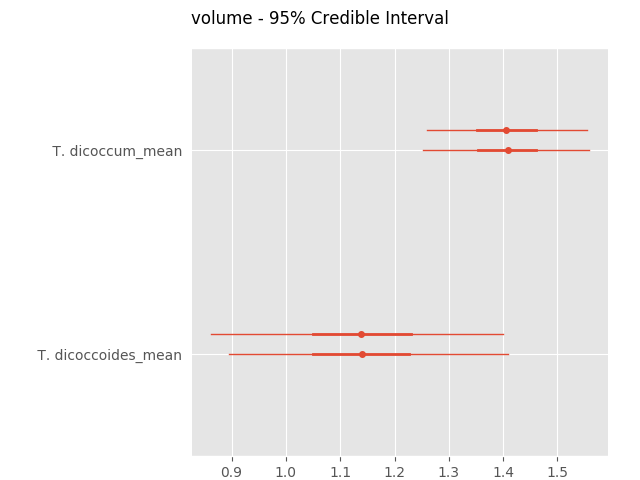
\includegraphics[width=0.45\textwidth]{./images/results/group2/bayes_volume.png}
  }
  \caption{Forest plots showing credible intervals of wild and domesticated genotypes for volume in (a) diploid (2N) grains,(b) tetraploid (4N) grains. (a) shows a 0.4\% chance of similar means  and (b) a 3.6\%}
  \label{fig:lenmeansvolume}
\end{figure}

The diploids show a 0.4\% chance of their means being similar, while the tetraploids show a 3.7\% chance of a same mean value.

\section{Hexaploid Genotypes Contain No Significant Variation}
\label{sec:org6371e2b}

Hexaploids \emph{T. aestivum} and \emph{T. spelta} are both elite cultivars. When compared show that there is a 77.2\% chance than there is a difference in the means of length. A 54.8\% chance of difference in width.

A 91.5\% chance and a 89.0\% chance of difference of means in volume and length X depth x width, respectively.

These values, with the exception of volume, do not provide sufficient evidence of significant variation in hexaploid varieties used in this study.


\clearpage


\section{Grain Volume Does Not Increase with Ploidy}
\label{sec:org0fd0027}

Diploids (\emph{T. beoticum}, \emph{T. monococcum}) , tetraploids (\emph{T. dicoccum}, \emph{T. dicoccoides})  show a significant difference in volume.

Hexaploids (\emph{T. aestivum}) when compared to tetraploids (\emph{T. dicoccum}) reports a 86.2\% chance of the two means being the same. Indicating that increasing of ploidy fron 4N to 6N does not produce a significant change in grain volume. Figure:\ref{fig:orgc3df192} shows this, with full results shown in supplemental figure:\ref{fig:group6}.

\begin{figure}[htbp]
\centering
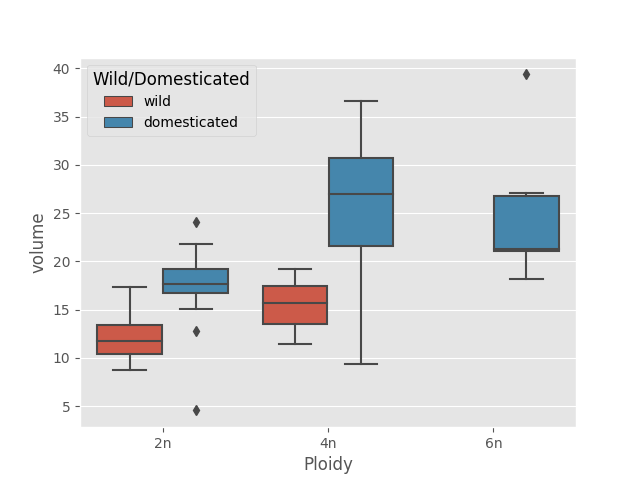
\includegraphics[width=10cm]{./images/results/ploidyvol.png}
\caption{\label{fig:orgc3df192}
A boxplot of all grains' volume plotted by ploidy and domestication status}
\end{figure}


Comparing \emph{T. durum} and \emph{T. aestivum} there is a 94.7\% chance that the means are similar, this indicates that volume is not dependant on ploidy fully.


\begin{figure}[htbp]
\centering
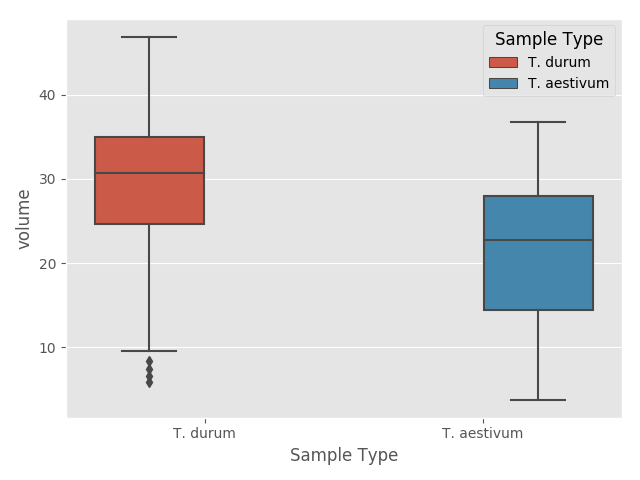
\includegraphics[width=8cm]{./images/results/group7/volume.png}
\caption{\label{fig:org5f2074c}
A boxplot of \emph{T. durum} and \emph{T. aestivum} volume}
\end{figure}

\clearpage
\chapter{Discussion}
\label{sec:org62f9fa1}

Here, this chapter will discuss the relevance of this research, its place in the wider field of plant sciences. The meaning of results and their agreement with current literature is also discussed. As well are some interesting findings, which while not statistically significant are cause of interest and further investigation.

\section{\textmu{}-CT As Tool For Exploring Domestication}
\label{sec:org35e1441}
In plant science \textmu{}-CT and other imaging techniques have been used to great effect \cite{Hubeau2015,Staedler2013,Metzner2015}. Here this project builds upon and adds to an established image analysis tool \cite{Hughes2017} where this method was designed for drought stress experiments this project has expanded functionality for use with a wide range of genotypes.

A wide range of attributes which previous studies could not access \cite{Gegas2010} is made available for study. In figure:\ref{fig:org9a4f6d7} the available phenotypes are displayed in a pairwise fashion, demonstrating how interesting relationships between attributes could provide more information if studied further.

The provided pairwise plots consist of scatter plots, each marker represents a single grain, and diagonals are kernel density estimation plots which show the distribution of the phenotypes. For each comparison group from the study a pairwise plot is provided in supplemental figures.

Primarily, this study has focused on the following phenotypes:

\begin{enumerate}
\item Length
\item Width
\item Volume
\item Surface Area
\end{enumerate}

Length and width have previously been studied through two dimensional imaging \cite{Gegas2010}, their availability through this method provides an interesting point of reference. Volume and surface area both present unstudied phenotypes. Grain studies often use spike weight or thousand-grain-weight (TGW) as an estimation of yield from crops, such large assumptions are unsuited when so much variation exists on a grain-to-grain basis. The relationship between spike weight and sum of spike volume has previously been shown to have been significantly correlated \cite{Hughes2017}. As such, this study proposes that grain volume is a much more useful measurement, reduces amount of data collection needed and that it can also be used as a proxy for TGW if required.

\begin{figure}[htbp]
\centering
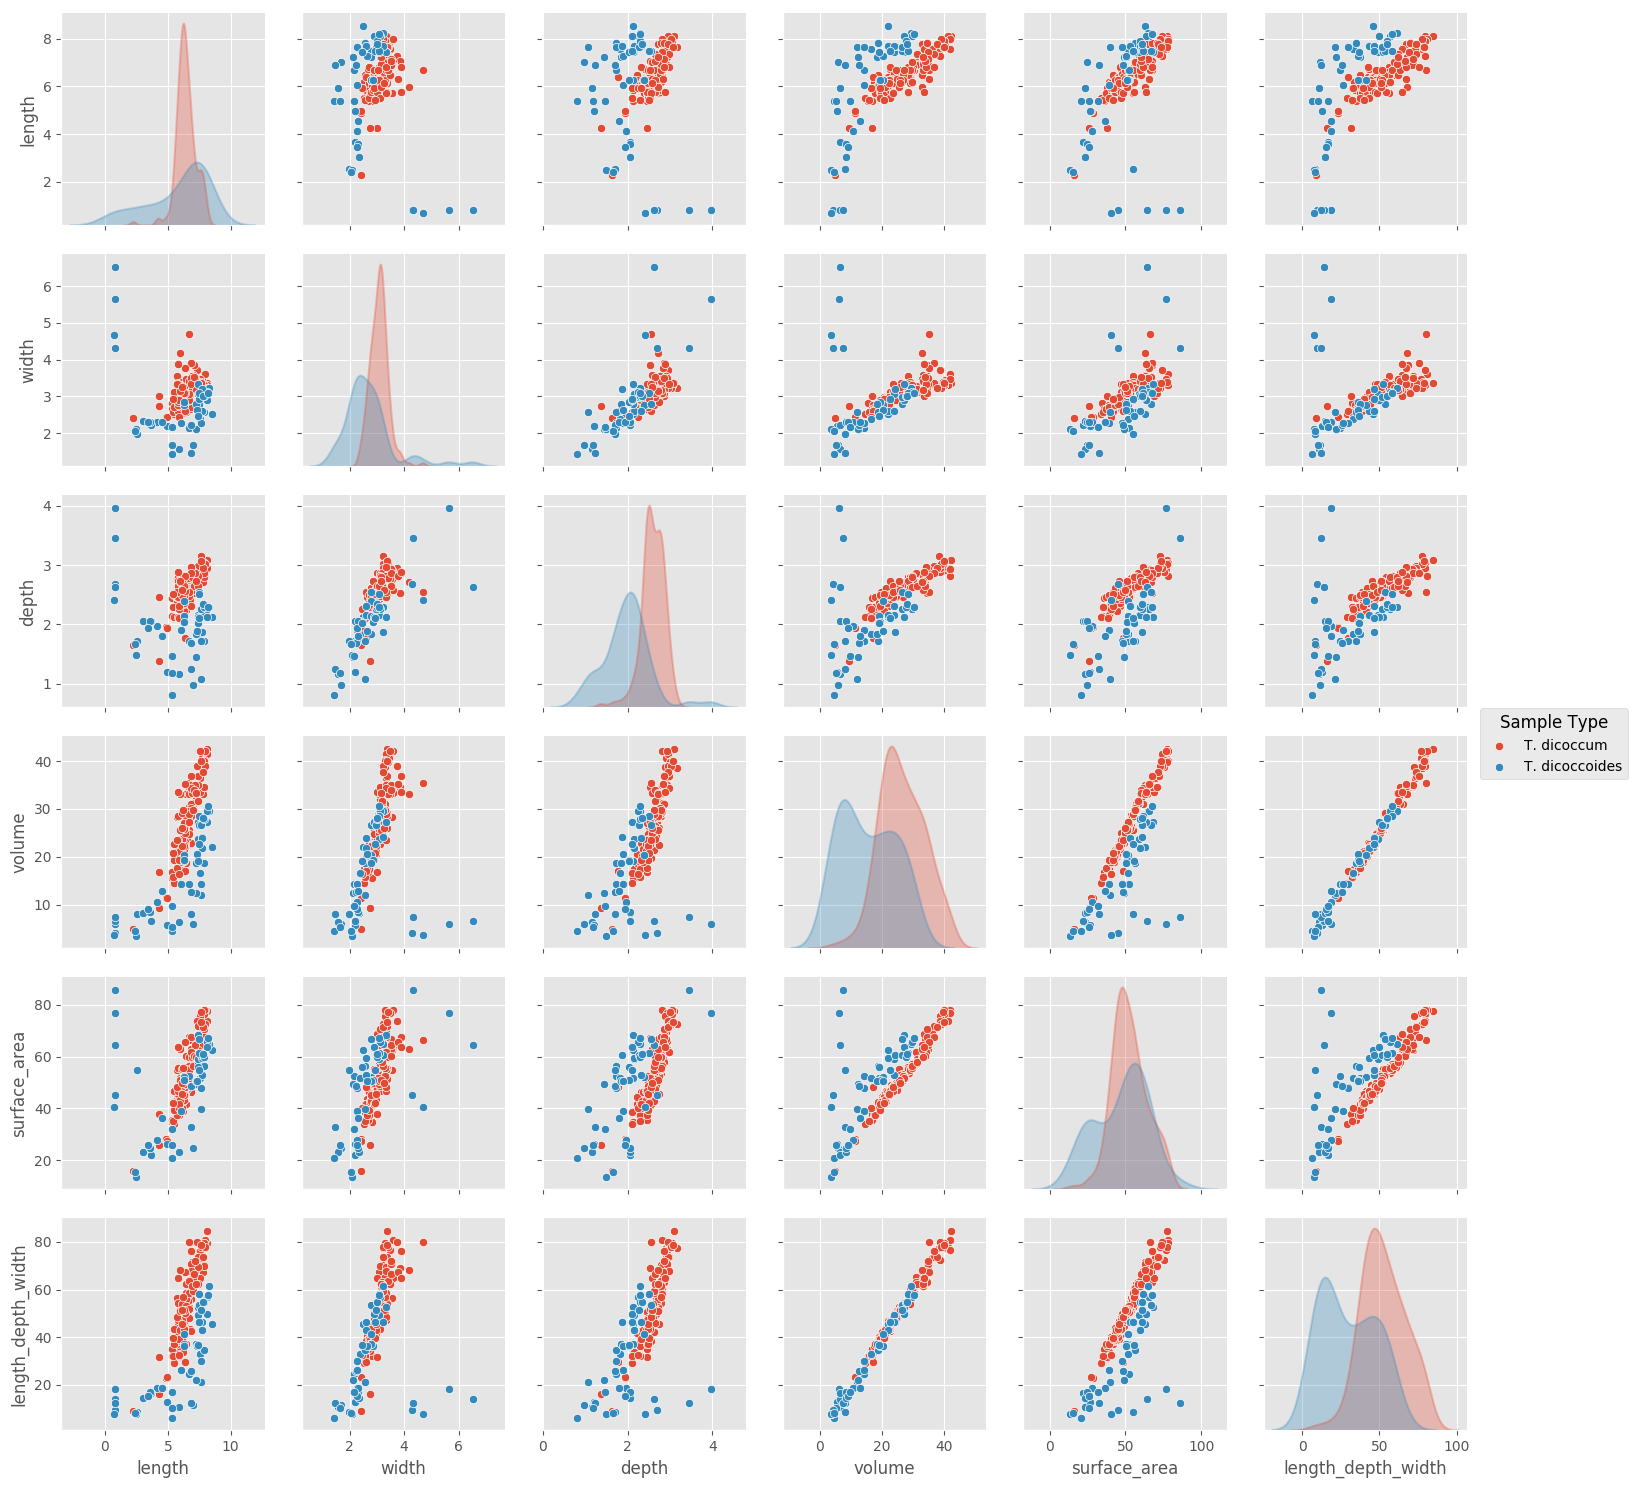
\includegraphics[width=18cm]{./images/results/group2/pairplot.png}
\caption{\label{fig:org9a4f6d7}
A pairplot of two tetraploid genotypes}
\end{figure}

\clearpage

\section{Effects of Ploidy on Grain Width}
\label{sec:orgb17f5a1}

Lin Qin et at. reported that an increased grain kernel width was observed in tetraploid genotypes. Furthermore, that this change can be accounted for by \emph{TaGW2} gene expression levels, where a decline was observed between diploid, tetraploid and hexaploid wheat \cite{Qin2017}.

It has been suggested that polyploidization events cause stronger effects in grain morphology than domestication or breeding \cite{Qin2017}. The data made available through this research has the potential to explore and contribute to this suggestion. Where similar effects have been observed but have not been cross compared to answer this question.

However, results from comparing primitive \emph{T. beoticum} and \emph{T. dicoccoides} show that an insignificant effect is present and that there is a high likelihood of width overlap. This effect could be down to a poor comparison choice as these genotypes may have arose from separate events \cite{Ozkan2002}.

\section{Grain Classification through PCA}
\label{sec:org53cf320}
Gegas et al. previously made great use of principal component analysis with wheat mapping populations. Using PCA afforded information on grain morphology specifically towards which traits could be traced to features from ancestral species.

With this data, similar solutions could be implemented. Figure:\ref{fig:org155d9f5} shows all grains in this study, grouped by origin spike and plotted by a two component PCA. Input is calculated through averaging across spike grains' length, width, depth, volume and the geometric interaction term, via equation:\ref{eq:org00f96ac}.

 \begin{align}
\label{eq:org00f96ac}
   &\begin{aligned}
\text{Phenotype}_i = \frac{1}{n}\times\sum^n_{j=1}{x^i_j}
   \end{aligned}
 \end{align}
\myequations{PCA Equation}


\begin{figure}[htbp]
\centering
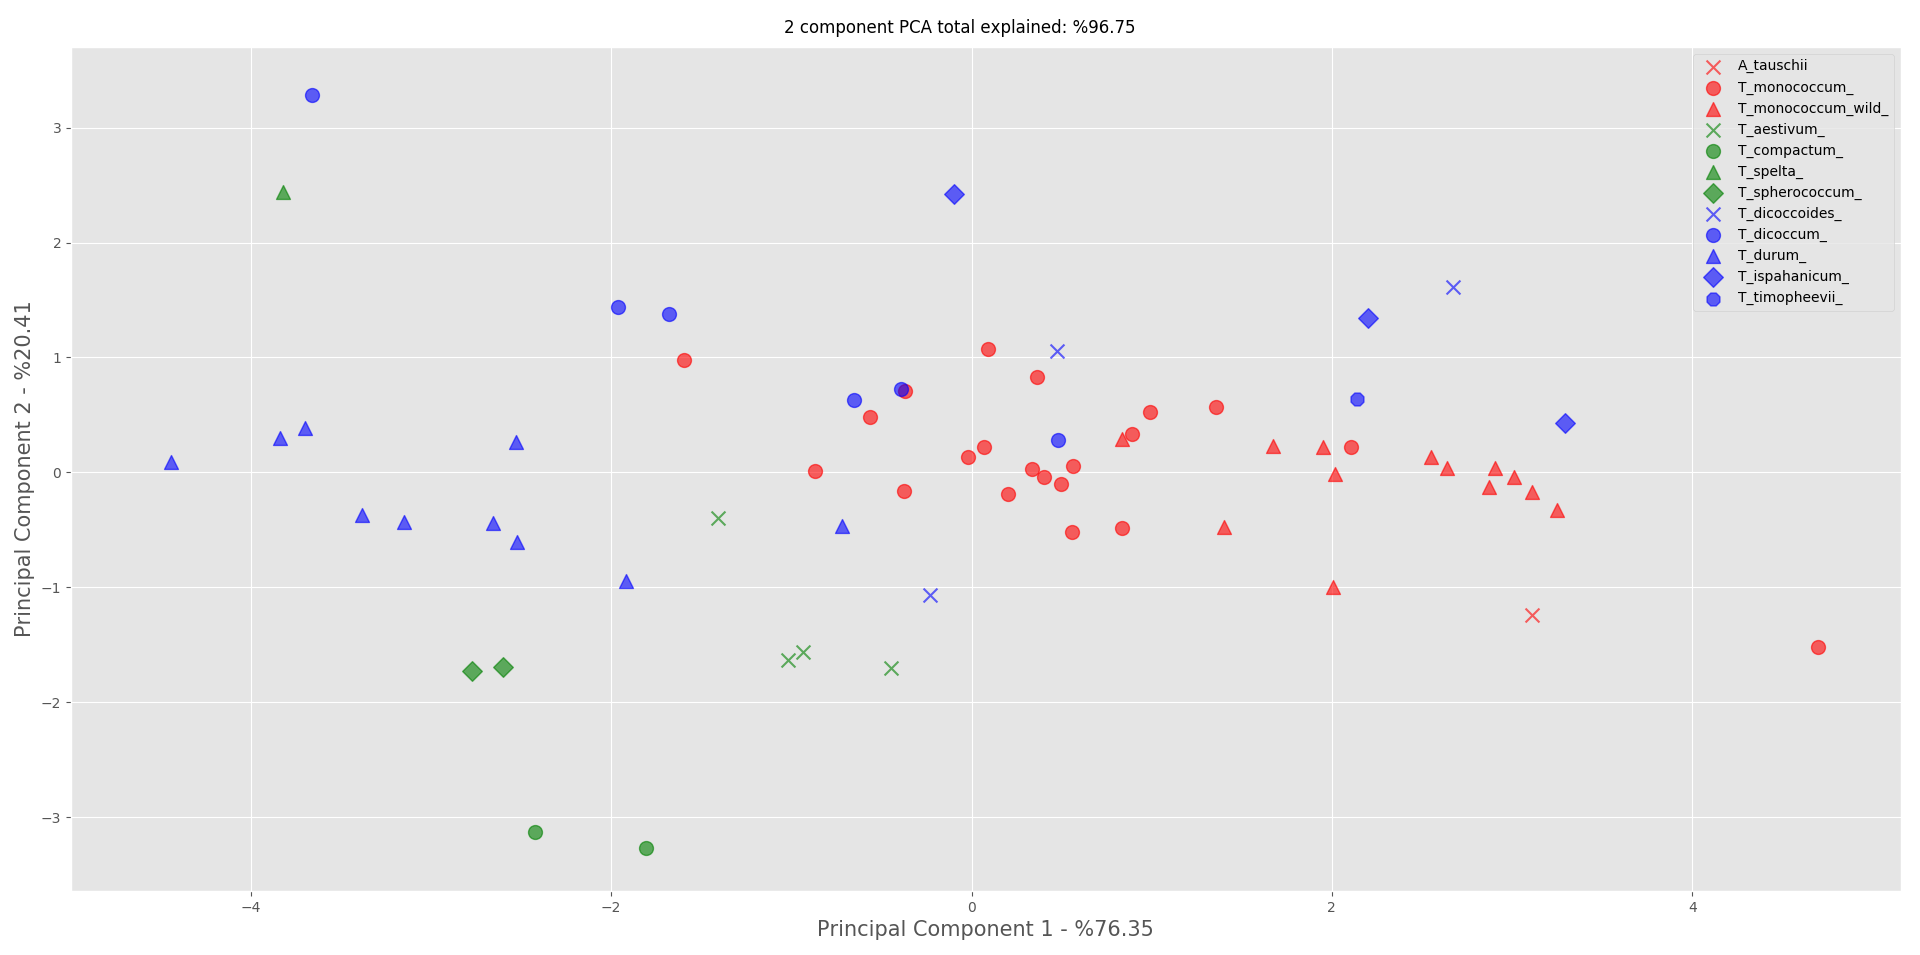
\includegraphics[width=.9\linewidth]{./images/pca_all.png}
\caption{\label{fig:org155d9f5}
A 2 component PCA showing all the spikes discussed in this study}
\end{figure}

\section{CT Library and CT GUI}
\label{sec:org8b55b27}

The library provided by this project ensures the standardisation and organising of \textmu{}-CT image data for crops. By creating a base line method of processing a lot of repeated work can be avoided. In addition it also provides a new hypothesis testing model which is yet unused in crop science or to study morphology in seeds. The introduction of a easy to use library will hopefully speed up future experiments and make them comparable to previous ones. This contributes to the robustness of the studies themselves and creates work which can be built upon.

The CT GUI application delivers a package in which a user can quickly view vast amounts of data, allowing clear and concise visual representation of thousands of seeds at once. Furthermore, this application gathers data and outputs it in a standard output, this allows for other external software such as \emph{R}-language packages or other \emph{Python} libraries to make use of it.

Both these pieces of software will be made freely available as research tools, the openness of them, and with the ability for others to modify and contribute to will ensure the ideologies of open science are kept.

Ideally a MIT style software license will be applied to these software packages, and they will also be made available on python library repositories for easy distribution


\chapter{Critical Evaluation}
\label{sec:orga827f2e}
\section{Organisational Methods}
\label{sec:org4e9265f}
\section{Relevance to Degree}
\label{sec:org7966887}
\section{Time Management}
\label{sec:org12a41eb}
\section{Collaborative Work}
\label{sec:org2a79afc}
\section{Other Issues}
\label{sec:org843e18a}


\appendix

\chapter{Glossary}
\label{sec:org45ffa6f}
\begin{table}[htbp]
\caption{\label{tab:org48f7e61}
Dictionary for Terms and acronyms}
\centering
\begin{tabularx}{\textwidth}{|l|X|}
\hline
\textbf{Term} & \textbf{Definition}\\
\hline
\textmu{}-CT & Micro Computed Tomography\\
\hline
Genotype & A genetically distinct individual or group\\
\hline
Phenotype & A physical/measurable trait\\
\hline
Alleles & A variant of a gene\\
\hline
Genus & Classification ranking, below the \emph{family} grouping\\
\hline
Genome & The complete genetic make up of an organism, which defines its individuality\\
\hline
Morphometric & The shape and form of an organism\\
\hline
GUI & Graphical User Interface\\
\hline
PCA & Principal Component Analysis\\
\hline
Spike & A singular stalk of wheat\\
\hline
Spikelet & A group of seeds all forming from the same node in a spike\\
\hline
MVC & Model View Controller - A design pattern for GUIs\\
\hline
OOP & Object Orientated Programming\\
\hline
\(X \sim \mathcal{N}(\mu,\,\sigma^{2})\) & Notation for Normal (Gaussian) Distribution\\
\hline
\end{tabularx}
\end{table}

\clearpage


\chapter{Libraries, Tools and Documentation}
\label{sec:org074b8b7}

\subsection{Libraries}
\label{sec:org658774c}
\begin{table}[htbp]
\caption{\label{tab:org8925f5a}
Software libraries used}
\centering
\begin{tabularx}{\textwidth}{|X|X|X|}
\hline
Seaborn & Scipy & Sklearn\\
\hline
MATLAB Image Processing Toolbox & Numpy & Matplotlib\\
\hline
Statsmodels & Pymc3 & Xlrd\\
\hline
PyQt5 & gcc & Pip\\
\hline
\end{tabularx}
\end{table}

\subsection{Tools}
\label{sec:orgc210de8}
\begin{table}[htbp]
\caption{\label{tab:org66c29b8}
Software tools used}
\centering
\begin{tabularx}{\textwidth}{|X|X|X|}
\hline
MATLAB & Python Debugger (PDB) & IPython\\
\hline
Emacs & git & org-mode\\
\hline
Tomviz & ImageJ & PlantUML\\
\hline
\end{tabularx}
\end{table}

\section{Documentation}
\label{sec:org524922d}
\clearpage

\chapter{Wheat Varieties}
\label{sec:org23d70e1}
\begin{table}[htbp]
\caption{\label{tab:orge0a0129}
Wheat used in this work and their common names}
\centering
\begin{tabularx}{\textwidth}{|X|X|}
\hline
\textbf{Species name} & \textbf{Common name}\\
\hline
\emph{Triticum monococcum} & Einkorn Domesticate\\
\hline
\emph{Triticum boeticum} & Einkorn Wild\\
\hline
\emph{Triticum durum} & Pasta Wheat\\
\hline
\emph{Triticum dicoccoides} & Emmer Domesticate\\
\hline
\emph{Triticum dicoccum} & Emmer Wild\\
\hline
\emph{Triticum ispahanicum} & n/a\\
\hline
\emph{Triticum timopheevii} & n/a\\
\hline
\emph{Triticum spelta} & Spelt\\
\hline
\emph{Triticum aestivum} & Bread Wheat\\
\hline
\emph{Triticum compactum} & Club Wheat\\
\hline
\end{tabularx}
\end{table}



\clearpage
\chapter{Code Segments and Examples}
\label{sec:orgb9b9e48}

\section{Setup.py}
\label{sec:orge48d769}
\begin{listing}[htbp]
\begin{minted}[linenos,firstnumber=1,frame=lines,linenos=true,fontfamily=DejaVuSans]{python}
from setuptools import setup
setup(name='CT_Analysing_Library',
      version='0.2',
      description='Library used for CT grain analysis at the NPPC',
      url='https://github.com/SirSharpest/CT_Analysing_Library',
      author='Nathan Hughes',
      author_email='nathan1hughes@gmail.com',
      license='MIT',
      packages=['ct_analysing_library'],
      install_requires=['pandas',
                        'numpy',
                        'matplotlib',
                        'seaborn',
                        'scipy',
                        'sklearn',
                        'statsmodels',
                        'pymc3',
                        'xlrd'],
      zip_safe=True)
\end{minted}
\caption{\label{org39ea4a7}
The \emph{setup.py} configuration for the CT Analyser Library}
\end{listing}

\clearpage
\section{Self-Documenting Code Example}
\label{sec:org5eb2d46}
\begin{listing}[htbp]
\begin{minted}[linenos,firstnumber=1,frame=lines,linenos=true,fontfamily=DejaVuSans]{python}
def get_spike_info(self, excel_file, join_column='Folder#'):
    """
    This function should do something akin to adding additional
    information to the data frame

    @note there is some confusion in the NPPC about whether to use
    folder name or file name as the unique id when this is made into
    end-user software, a toggle should be added to allow this

    @param excel_file a file to attach and read data from
    @param join_column if the column for joining data is
    different then it should be stated
    """
        # Grab the linking excel file
        info = pd.read_excel(excel_file,
                             index_col='Folder#')

        features = list(info.columns)
        # Lambda to look up the feature in excel spreadsheet
        def look_up(x, y): return info.loc[x['folderid']][y]

        # Lambda form a series (data row) and apply it to dataframe
        def gather_data(x): return pd.Series(
            [look_up(x, y) for y in features])

        self.df[features] = self.df.apply(gather_data, axis=1)
    except KeyError as e:
        print('Error matching data')
        print(e)
        raise NoDataFoundException
    except AttributeError as e:
        print(e)
        raise NoDataFoundException

\end{minted}
\caption{\label{orgeb46770}
Example of code documentation and readability from \emph{data\_transforms.py}}
\end{listing}
\clearpage


\section{Custom Documentation Generator}
\label{sec:org8ac4426}
\begin{listing}[htbp]
\begin{minted}[linenos,firstnumber=1,frame=lines,linenos=true,fontfamily=DejaVuSans]{common-lisp}
(defun populate-org-buffer (buffer filename root)
  (goto-char (point-min))
  (let ((to-insert (concat "* " (replace-regexp-in-string root "" filename) "\n") ))
    (while (re-search-forward
            (rx (group (or "def" "class"))
                space
                (group (+ (not (any "()"))))
                (? "(" (* nonl) "):" (+ "\n") (+ space)
                   (= 3 "\"")
                   (group (+? anything))
                   (= 3 "\"")))
            nil 'noerror)
      (setq to-insert
            (concat
             to-insert
             (if (string= "class" (match-string 1))
                 "** "
               "*** ")
             (match-string 2)
             "\n"
             (and (match-string 3)
                  (concat (match-string 3) "\n")))))helm-semantic-or-imenu
    (with-current-buffer buffer
      (insert to-insert))))
(defun org-documentation-from-dir (&optional dir)
  (interactive)
  (let* ((dir  (or dir (read-directory-name "Choose base directory: ")))
         (files (directory-files-recursively dir "\py$"))
         (doc-buf (get-buffer-create "org-docs")))
    (dolist (file files)
      (with-temp-buffer
        (insert-file-contents file)
        (populate-org-buffer doc-buf file dir)))
    (with-current-buffer doc-buf
      (org-mode))))
\end{minted}
\caption{\label{orgaf430bd}
Custom lisp code for generating easy to read documentation}
\end{listing}

\clearpage
\chapter{Full Comparison Plots}
\label{sec:orgbde7757}
\section{\emph{T. monococcum} and \emph{T. beoticum}}
\label{sec:org578d101}

\subsection{Data Distributions}
\label{sec:org97aa6a5}

\begin{figure}[!ht]
  \subfloat[Boxplot of \textit{T. monococcum} and \textit{T. beoticum} Length  \label{subfig-1:length}]{%
    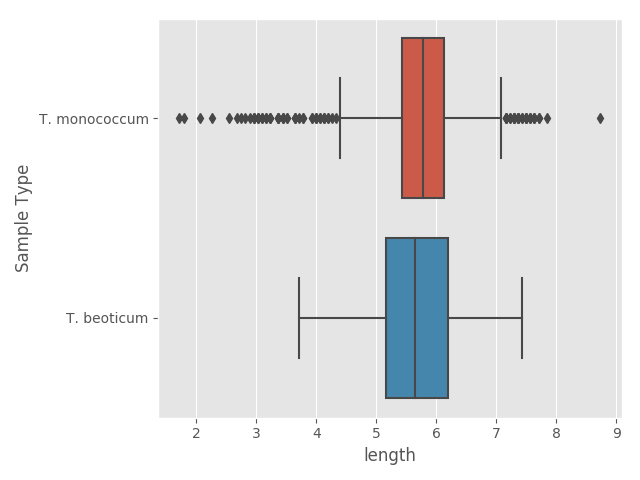
\includegraphics[width=0.45\textwidth]{./images/results/group1/length.png}
  }
  \hfill
  \subfloat[Boxplot of \textit{T. monococcum} and \textit{T. beoticum} Width  \label{subfig-2:Width}]{%
    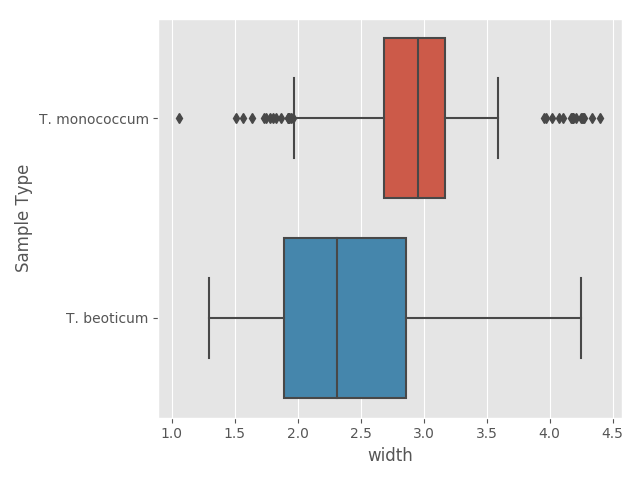
\includegraphics[width=0.45\textwidth]{./images/results/group1/width.png}
  }
  \hfill
  \subfloat[Boxplot of \textit{T. monococcum} and \textit{T. beoticum} Volume  \label{subfig-3:volume}]{%
    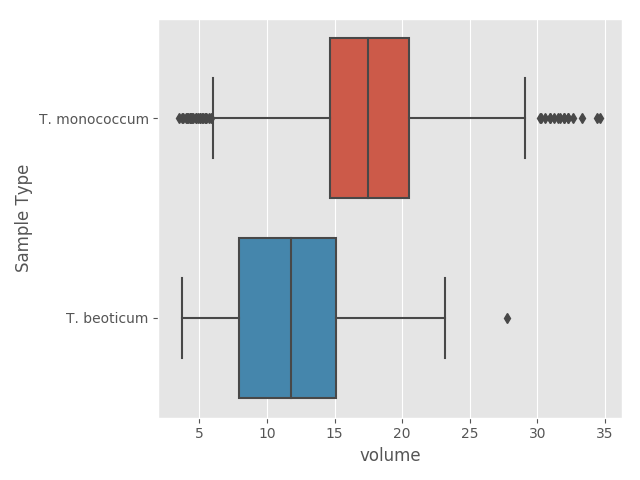
\includegraphics[width=0.45\textwidth]{./images/results/group1/volume.png}
  }
  \hfill
  \subfloat[Boxplot of \textit{T. monococcum} and \textit{T. beoticum} Length X depth X width \label{subfig-4:lengthwidthdepth}]{%
    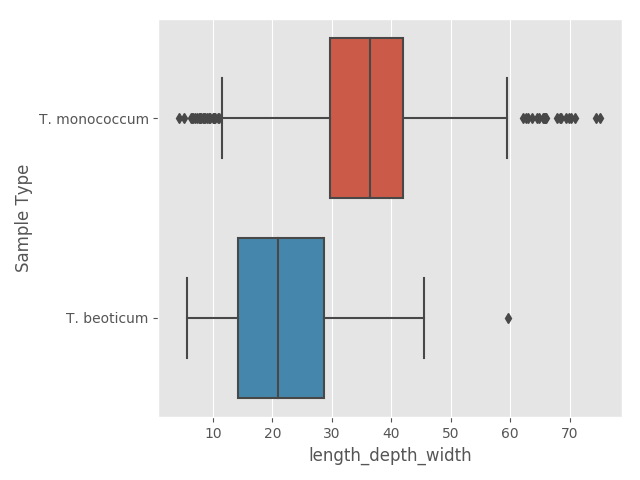
\includegraphics[width=0.45\textwidth]{./images/results/group1/length_depth_width.png}
    }
  \caption{Plots comparing means and distributions of \textit{T. monococcum} (red) and \textit{T. beoticum} (blue)}
  \label{fig:dummy}
\end{figure}
\clearpage
\subsection{Difference of Means}
\label{sec:org98768de}

\begin{figure}[!ht]
  \subfloat[Difference of means for \textit{T. monococcum} and \textit{T. beoticum} Length  \label{subfig-1:length}]{%
    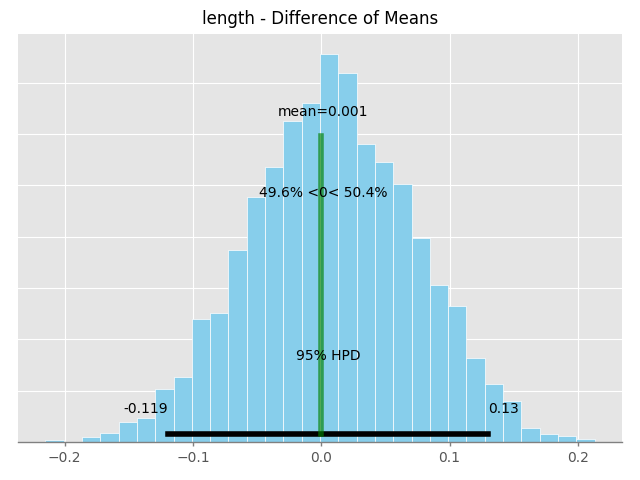
\includegraphics[width=0.45\textwidth]{./images/results/group1/bayes_difference_of_means_length.png}
  }
  \hfill
  \subfloat[Difference of means for \textit{T. monococcum} and \textit{T. beoticum} Width  \label{subfig-2:Width}]{%
    \includegraphics[width=0.45\textwidth]{./images/results/group1/bayes_difference_of_means_width.png}
  }
  \hfill
  \subfloat[Difference of means for \textit{T. monococcum} and \textit{T. beoticum} Volume  \label{subfig-3:volume}]{%
    \includegraphics[width=0.45\textwidth]{./images/results/group1/bayes_difference_of_means_volume.png}
  }
  \hfill
  \subfloat[Difference of means for \textit{T. monococcum} and \textit{T. beoticum} Length X depth X width \label{subfig-4:lengthwidthdepth}]{%
    \includegraphics[width=0.45\textwidth]{./images/results/group1/bayes_difference_of_means_length_depth_width.png}
    }
  \caption{Plots showing the differnce of means for  \textit{T. monococcum} -  \textit{T. beoticum}}
  \label{fig:group1}
\end{figure}
\clearpage
\subsection{Credible Intervals}
\label{sec:orgf9de6f4}
\begin{figure}[!ht]
  \subfloat[Credile Intervals for \textit{T. monococcum} and \textit{T. beoticum} Length  \label{subfig-1:length}]{%
    \includegraphics[width=0.45\textwidth]{./images/results/group1/bayes_length.png}
  }
  \hfill
  \subfloat[Credile Intervals for \textit{T. monococcum} and \textit{T. beoticum} Width  \label{subfig-2:Width}]{%
    \includegraphics[width=0.45\textwidth]{./images/results/group1/bayes_width.png}
  }
  \hfill
  \subfloat[Credile Intervals for \textit{T. monococcum} and \textit{T. beoticum} Volume  \label{subfig-3:volume}]{%
    \includegraphics[width=0.45\textwidth]{./images/results/group1/bayes_volume.png}
  }
  \hfill
  \subfloat[Credile Intervals for \textit{T. monococcum} and \textit{T. beoticum} Length X depth X width \label{subfig-4:lengthwidthdepth}]{%
    \includegraphics[width=0.45\textwidth]{./images/results/group1/bayes_length_depth_width.png}
    }
  \caption{Plots showing credible intervals for  \textit{T. monococcum} and  \textit{T. beoticum}}
  \label{fig:group1}
\end{figure}
\clearpage


\subsection{Pair Plot}
\label{sec:orgd859d1a}

\begin{figure}[htbp]
\centering
\includegraphics[width=18cm]{./images/results/group1/pairplot.png}
\label{fig:org04298e6}
\end{figure}

\clearpage
\subsection{PCA}
\label{sec:orgd68409a}
\begin{figure}[htbp]
\centering
\includegraphics[width=18cm]{./images/results/group1/pca.png}
\label{fig:org0e0823a}
\end{figure}

\clearpage
\section{\emph{T. dicoccum} and \emph{T. dicoccoides}}
\label{sec:org7e45b2d}

\subsection{Data Distributions}
\label{sec:org21e3ad4}

\begin{figure}[!ht]
  \subfloat[Boxplot of \textit{T. dicoccum} and \textit{T. dicoccoides} Length  \label{subfig-1:length}]{%
    \includegraphics[width=0.45\textwidth]{./images/results/group2/length.png}
  }
  \hfill
  \subfloat[Boxplot of \textit{T. dicoccum} and \textit{T. dicoccoides} Width  \label{subfig-2:Width}]{%
    \includegraphics[width=0.45\textwidth]{./images/results/group2/width.png}
  }
  \hfill
  \subfloat[Boxplot of \textit{T. dicoccum} and \textit{T. dicoccoides} Volume  \label{subfig-3:volume}]{%
    \includegraphics[width=0.45\textwidth]{./images/results/group2/volume.png}
  }
  \hfill
  \subfloat[Boxplot of \textit{T. dicoccum} and \textit{T. dicoccoides} Length X depth X width \label{subfig-4:lengthwidthdepth}]{%
    \includegraphics[width=0.45\textwidth]{./images/results/group2/length_depth_width.png}
    }
  \caption{Plots comparing means and distributions of \textit{T. dicoccum} (red) and \textit{T. dicoccoides} (blue)}
  \label{fig:dummy}
\end{figure}
\clearpage
\subsection{Difference of Means}
\label{sec:org76e7d10}

\begin{figure}[!ht]
  \subfloat[Difference of means for \textit{T. dicoccum} and \textit{T. dicoccoides} Length  \label{subfig-1:length}]{%
    \includegraphics[width=0.45\textwidth]{./images/results/group2/bayes_difference_of_means_length.png}
  }
  \hfill
  \subfloat[Difference of means for \textit{T. dicoccum} and \textit{T. dicoccoides} Width  \label{subfig-2:Width}]{%
    \includegraphics[width=0.45\textwidth]{./images/results/group2/bayes_difference_of_means_width.png}
  }
  \hfill
  \subfloat[Difference of means for \textit{T. dicoccum} and \textit{T. dicoccoides} Volume  \label{subfig-3:volume}]{%
    \includegraphics[width=0.45\textwidth]{./images/results/group2/bayes_difference_of_means_volume.png}
  }
  \hfill
  \subfloat[Difference of means for \textit{T. dicoccum} and \textit{T. dicoccoides} Length X depth X width \label{subfig-4:lengthwidthdepth}]{%
    \includegraphics[width=0.45\textwidth]{./images/results/group2/bayes_difference_of_means_length_depth_width.png}
    }
  \caption{Plots showing the differnce of means for  \textit{T. dicoccum} -  \textit{T. dicoccoides}}
  \label{fig:group2}
\end{figure}
\clearpage

\subsection{Credible Intervals}
\label{sec:org2496ddf}

\begin{figure}[!ht]
  \subfloat[Credible Intervalsfor \textit{T. dicoccum} and \textit{T. dicoccoides} Length  \label{subfig-1:length}]{%
    \includegraphics[width=0.45\textwidth]{./images/results/group2/bayes_length.png}
  }
  \hfill
  \subfloat[Credible Intervalsfor \textit{T. dicoccum} and \textit{T. dicoccoides} Width  \label{subfig-2:Width}]{%
    \includegraphics[width=0.45\textwidth]{./images/results/group2/bayes_width.png}
  }
  \hfill
  \subfloat[Credible Intervalsfor \textit{T. dicoccum} and \textit{T. dicoccoides} Volume  \label{subfig-3:volume}]{%
    \includegraphics[width=0.45\textwidth]{./images/results/group2/bayes_volume.png}
  }
  \hfill
  \subfloat[Credible Intervalsfor \textit{T. dicoccum} and \textit{T. dicoccoides} Length X depth X width \label{subfig-4:lengthwidthdepth}]{%
    \includegraphics[width=0.45\textwidth]{./images/results/group2/bayes_length_depth_width.png}
    }
  \caption{Plots showing credible intervals for  \textit{T. dicoccum} and  \textit{T. dicoccoides}}
  \label{fig:group2}
\end{figure}
\clearpage




\subsection{Pair Plot}
\label{sec:org2f74bf1}

\begin{figure}[htbp]
\centering
\includegraphics[width=18cm]{./images/results/group2/pairplot.png}
\label{fig:orgce0fb83}
\end{figure}

\clearpage
\subsection{PCA}
\label{sec:org94e4cd1}
\begin{figure}[htbp]
\centering
\includegraphics[width=18cm]{./images/results/group2/pca.png}
\label{fig:org926b01b}
\end{figure}



\clearpage
\section{\emph{T. spelta} and \emph{T. aestivum}}
\label{sec:org0fbd08e}

\subsection{Data Distributions}
\label{sec:org656a7fd}

\begin{figure}[!ht]
  \subfloat[Boxplot of \textit{T. spelta} and \textit{T. aestivum} Length  \label{subfig-1:length}]{%
    \includegraphics[width=0.45\textwidth]{./images/results/group3/length.png}
  }
  \hfill
  \subfloat[Boxplot of \textit{T. spelta} and \textit{T. aestivum} Width  \label{subfig-2:Width}]{%
    \includegraphics[width=0.45\textwidth]{./images/results/group3/width.png}
  }
  \hfill
  \subfloat[Boxplot of \textit{T. spelta} and \textit{T. aestivum} Volume  \label{subfig-3:volume}]{%
    \includegraphics[width=0.45\textwidth]{./images/results/group3/volume.png}
  }
  \hfill
  \subfloat[Boxplot of \textit{T. spelta} and \textit{T. aestivum} Length X depth X width \label{subfig-4:lengthwidthdepth}]{%
    \includegraphics[width=0.45\textwidth]{./images/results/group3/length_depth_width.png}
    }
  \caption{Plots comparing means and distributions of \textit{T. spelta} (red) and \textit{T. aestivum} (blue)}
  \label{fig:dummy}
\end{figure}
\clearpage
\subsection{Difference of Means}
\label{sec:org8c3ba58}

\begin{figure}[!ht]
  \subfloat[Difference of means for \textit{T. spelta} and \textit{T. aestivum} Length  \label{subfig-1:length}]{%
    \includegraphics[width=0.45\textwidth]{./images/results/group3/bayes_difference_of_means_length.png}
  }
  \hfill
  \subfloat[Difference of means for \textit{T. spelta} and \textit{T. aestivum} Width  \label{subfig-2:Width}]{%
    \includegraphics[width=0.45\textwidth]{./images/results/group3/bayes_difference_of_means_width.png}
  }
  \hfill
  \subfloat[Difference of means for \textit{T. spelta} and \textit{T. aestivum} Volume  \label{subfig-3:volume}]{%
    \includegraphics[width=0.45\textwidth]{./images/results/group3/bayes_difference_of_means_volume.png}
  }
  \hfill
  \subfloat[Difference of means for \textit{T. spelta} and \textit{T. aestivum} Length X depth X width \label{subfig-4:lengthwidthdepth}]{%
    \includegraphics[width=0.45\textwidth]{./images/results/group3/bayes_difference_of_means_length_depth_width.png}
    }
  \caption{Plots showing the differnce of means for  \textit{T. spelta} -  \textit{T. aestivum}}
  \label{fig:group3}
\end{figure}
\clearpage



\subsection{Credible Intervals}
\label{sec:orge681c71}

\begin{figure}[!ht]
  \subfloat[Credible Intervals for \textit{T. spelta} and \textit{T. aestivum} Length  \label{subfig-1:length}]{%
    \includegraphics[width=0.45\textwidth]{./images/results/group3/bayes_length.png}
  }
  \hfill
  \subfloat[Credible Intervals for \textit{T. spelta} and \textit{T. aestivum} Width  \label{subfig-2:Width}]{%
    \includegraphics[width=0.45\textwidth]{./images/results/group3/bayes_width.png}
  }
  \hfill
  \subfloat[Credible Intervals for \textit{T. spelta} and \textit{T. aestivum} Volume  \label{subfig-3:volume}]{%
    \includegraphics[width=0.45\textwidth]{./images/results/group3/bayes_volume.png}
  }
  \hfill
  \subfloat[Credible Intervals for \textit{T. spelta} and \textit{T. aestivum} Length X depth X width \label{subfig-4:lengthwidthdepth}]{%
    \includegraphics[width=0.45\textwidth]{./images/results/group3/bayes_length_depth_width.png}
    }
  \caption{Plots showing the credible intervals for  \textit{T. spelta} and  \textit{T. aestivum}}
  \label{fig:group3}
\end{figure}
\clearpage


\subsection{Pair Plot}
\label{sec:org789343d}

\begin{figure}[htbp]
\centering
\includegraphics[width=18cm]{./images/results/group3/pairplot.png}
\label{fig:orgd807d6e}
\end{figure}

\clearpage
\subsection{PCA}
\label{sec:org7eb3cd2}
\begin{figure}[htbp]
\centering
\includegraphics[width=18cm]{./images/results/group3/pca.png}
\label{fig:org935117f}
\end{figure}


\clearpage
\section{\emph{T. beoticum} and \emph{T. dicoccoides}}
\label{sec:orge23f08a}

\subsection{Data Distributions}
\label{sec:org77ab4b3}

\begin{figure}[!ht]
  \subfloat[Boxplot of \textit{T. beoticum} and \textit{T. dicoccoides} Length  \label{subfig-1:length}]{%
    \includegraphics[width=0.45\textwidth]{./images/results/group4/length.png}
  }
  \hfill
  \subfloat[Boxplot of \textit{T. beoticum} and \textit{T. dicoccoides} Width  \label{subfig-2:Width}]{%
    \includegraphics[width=0.45\textwidth]{./images/results/group4/width.png}
  }
  \hfill
  \subfloat[Boxplot of \textit{T. beoticum} and \textit{T. dicoccoides} Volume  \label{subfig-3:volume}]{%
    \includegraphics[width=0.45\textwidth]{./images/results/group4/volume.png}
  }
  \hfill
  \subfloat[Boxplot of \textit{T. beoticum} and \textit{T. dicoccoides} Length X depth X width \label{subfig-4:lengthwidthdepth}]{%
    \includegraphics[width=0.45\textwidth]{./images/results/group4/length_depth_width.png}
    }
  \caption{Plots comparing means and distributions of \textit{T. beoticum} (red) and \textit{T. dicoccoides} (blue)}
  \label{fig:dummy}
\end{figure}
\clearpage
\subsection{Difference of Means}
\label{sec:org556eb78}

\begin{figure}[!ht]
  \subfloat[Difference of means for \textit{T. beoticum} and \textit{T. dicoccoides} Length  \label{subfig-1:length}]{%
    \includegraphics[width=0.45\textwidth]{./images/results/group4/bayes_difference_of_means_length.png}
  }
  \hfill
  \subfloat[Difference of means for \textit{T. beoticum} and \textit{T. dicoccoides} Width  \label{subfig-2:Width}]{%
    \includegraphics[width=0.45\textwidth]{./images/results/group4/bayes_difference_of_means_width.png}
  }
  \hfill
  \subfloat[Difference of means for \textit{T. beoticum} and \textit{T. dicoccoides} Volume  \label{subfig-3:volume}]{%
    \includegraphics[width=0.45\textwidth]{./images/results/group4/bayes_difference_of_means_volume.png}
  }
  \hfill
  \subfloat[Difference of means for \textit{T. beoticum} and \textit{T. dicoccoides} Length X depth X width \label{subfig-4:lengthwidthdepth}]{%
    \includegraphics[width=0.45\textwidth]{./images/results/group4/bayes_difference_of_means_length_depth_width.png}
    }
  \caption{Plots showing the differnce of means for  \textit{T. beoticum} -  \textit{T. dicoccoides}}
  \label{fig:group4}
\end{figure}
\clearpage


\subsection{Credible Intervals}
\label{sec:org835f502}

\begin{figure}[!ht]
  \subfloat[Credible Intervals for \textit{T. beoticum} and \textit{T. dicoccoides} Length  \label{subfig-1:length}]{%
    \includegraphics[width=0.45\textwidth]{./images/results/group4/bayes_length.png}
  }
  \hfill
  \subfloat[Credible Intervals for \textit{T. beoticum} and \textit{T. dicoccoides} Width  \label{subfig-2:Width}]{%
    \includegraphics[width=0.45\textwidth]{./images/results/group4/bayes_width.png}
  }
  \hfill
  \subfloat[Credible Intervals for \textit{T. beoticum} and \textit{T. dicoccoides} Volume  \label{subfig-3:volume}]{%
    \includegraphics[width=0.45\textwidth]{./images/results/group4/bayes_volume.png}
  }
  \hfill
  \subfloat[Credible Intervals for \textit{T. beoticum} and \textit{T. dicoccoides} Length X depth X width \label{subfig-4:lengthwidthdepth}]{%
    \includegraphics[width=0.45\textwidth]{./images/results/group4/bayes_length_depth_width.png}
    }
  \caption{Plots showing the credible intervals for  \textit{T. beoticum} and  \textit{T. dicoccoides}}
  \label{fig:group4}
\end{figure}
\clearpage



\subsection{Pair Plot}
\label{sec:orga1a94e6}

\begin{figure}[htbp]
\centering
\includegraphics[width=18cm]{./images/results/group4/pairplot.png}
\label{fig:orgf0126a9}
\end{figure}

\clearpage
\subsection{PCA}
\label{sec:org4302026}
\begin{figure}[htbp]
\centering
\includegraphics[width=18cm]{./images/results/group4/pca.png}
\label{fig:org4109452}
\end{figure}


\clearpage
\section{\emph{T. dicoccum} and \emph{T. durum}}
\label{sec:orgbea187c}

\subsection{Data Distributions}
\label{sec:org0fea18f}

\begin{figure}[!ht]
  \subfloat[Boxplot of \textit{T. dicoccum} and \textit{T. durum} Length  \label{subfig-1:length}]{%
    \includegraphics[width=0.45\textwidth]{./images/results/group5/length.png}
  }
  \hfill
  \subfloat[Boxplot of \textit{T. dicoccum} and \textit{T. durum} Width  \label{subfig-2:Width}]{%
    \includegraphics[width=0.45\textwidth]{./images/results/group5/width.png}
  }
  \hfill
  \subfloat[Boxplot of \textit{T. dicoccum} and \textit{T. durum} Volume  \label{subfig-3:volume}]{%
    \includegraphics[width=0.45\textwidth]{./images/results/group5/volume.png}
  }
  \hfill
  \subfloat[Boxplot of \textit{T. dicoccum} and \textit{T. durum} Length X depth X width \label{subfig-4:lengthwidthdepth}]{%
    \includegraphics[width=0.45\textwidth]{./images/results/group5/length_depth_width.png}
    }
  \caption{Plots comparing means and distributions of \textit{T. dicoccum} (red) and \textit{T. durum} (blue)}
  \label{fig:dummy}
\end{figure}
\clearpage
\subsection{Difference of Means}
\label{sec:org502b1db}

\begin{figure}[!ht]
  \subfloat[Difference of means for \textit{T. dicoccum} and \textit{T. durum} Length  \label{subfig-1:length}]{%
    \includegraphics[width=0.45\textwidth]{./images/results/group5/bayes_difference_of_means_length.png}
  }
  \hfill
  \subfloat[Difference of means for \textit{T. dicoccum} and \textit{T. durum} Width  \label{subfig-2:Width}]{%
    \includegraphics[width=0.45\textwidth]{./images/results/group5/bayes_difference_of_means_width.png}
  }
  \hfill
  \subfloat[Difference of means for \textit{T. dicoccum} and \textit{T. durum} Volume  \label{subfig-3:volume}]{%
    \includegraphics[width=0.45\textwidth]{./images/results/group5/bayes_difference_of_means_volume.png}
  }
  \hfill
  \subfloat[Difference of means for \textit{T. dicoccum} and \textit{T. durum} Length X depth X width \label{subfig-4:lengthwidthdepth}]{%
    \includegraphics[width=0.45\textwidth]{./images/results/group5/bayes_difference_of_means_length_depth_width.png}
    }
  \caption{Plots showing the differnce of means for  \textit{T. dicoccum} -  \textit{T. durum}}
  \label{fig:group5}
\end{figure}
\clearpage

\subsection{Credible Intervals}
\label{sec:org0b0e647}

\begin{figure}[!ht]
  \subfloat[Credible Intervals for for \textit{T. dicoccum} and \textit{T. durum} Length  \label{subfig-1:length}]{%
    \includegraphics[width=0.45\textwidth]{./images/results/group5/bayes_length.png}
  }
  \hfill
  \subfloat[Credible Intervals for for \textit{T. dicoccum} and \textit{T. durum} Width  \label{subfig-2:Width}]{%
    \includegraphics[width=0.45\textwidth]{./images/results/group5/bayes_width.png}
  }
  \hfill
  \subfloat[Credible Intervals for for \textit{T. dicoccum} and \textit{T. durum} Volume  \label{subfig-3:volume}]{%
    \includegraphics[width=0.45\textwidth]{./images/results/group5/bayes_volume.png}
  }
  \hfill
  \subfloat[Credible Intervals for for \textit{T. dicoccum} and \textit{T. durum} Length X depth X width \label{subfig-4:lengthwidthdepth}]{%
    \includegraphics[width=0.45\textwidth]{./images/results/group5/bayes_length_depth_width.png}
    }
  \caption{Plots showing the credible intervals for  \textit{T. dicoccum} and  \textit{T. durum}}
  \label{fig:group5}
\end{figure}
\clearpage



\subsection{Pair Plot}
\label{sec:org1cf84a1}

\begin{figure}[htbp]
\centering
\includegraphics[width=18cm]{./images/results/group5/pairplot.png}
\label{fig:org75ad873}
\end{figure}

\clearpage
\subsection{PCA}
\label{sec:org7b2de85}
\begin{figure}[htbp]
\centering
\includegraphics[width=18cm]{./images/results/group5/pca.png}
\label{fig:org7991465}
\end{figure}

\clearpage


\section{\emph{T. dicoccum} and \emph{T. aestivum}}
\label{sec:org084928e}

\subsection{Data Distributions}
\label{sec:org03315ef}

\begin{figure}[!ht]
  \subfloat[Boxplot of \textit{T. dicoccum} and \textit{T. aestivum} Length  \label{subfig-1:length}]{%
    \includegraphics[width=0.45\textwidth]{./images/results/group6/length.png}
  }
  \hfill
  \subfloat[Boxplot of \textit{T. dicoccum} and \textit{T. aestivum} Width  \label{subfig-2:Width}]{%
    \includegraphics[width=0.45\textwidth]{./images/results/group6/width.png}
  }
  \hfill
  \subfloat[Boxplot of \textit{T. dicoccum} and \textit{T. aestivum} Volume  \label{subfig-3:volume}]{%
    \includegraphics[width=0.45\textwidth]{./images/results/group6/volume.png}
  }
  \hfill
  \subfloat[Boxplot of \textit{T. dicoccum} and \textit{T. aestivum} Length X depth X width \label{subfig-4:lengthwidthdepth}]{%
    \includegraphics[width=0.45\textwidth]{./images/results/group6/length_depth_width.png}
    }
  \caption{Plots comparing means and distributions of \textit{T. dicoccum} (red) and \textit{T. aestivum} (blue)}
  \label{fig:dummy}
\end{figure}
\clearpage
\subsection{Difference of Means}
\label{sec:orgba8e2e4}

\begin{figure}[!ht]
  \subfloat[Difference of means for \textit{T. dicoccum} and \textit{T. aestivum} Length  \label{subfig-1:length}]{%
    \includegraphics[width=0.45\textwidth]{./images/results/group6/bayes_difference_of_means_length.png}
  }
  \hfill
  \subfloat[Difference of means for \textit{T. dicoccum} and \textit{T. aestivum} Width  \label{subfig-2:Width}]{%
    \includegraphics[width=0.45\textwidth]{./images/results/group6/bayes_difference_of_means_width.png}
  }
  \hfill
  \subfloat[Difference of means for \textit{T. dicoccum} and \textit{T. aestivum} Volume  \label{subfig-3:volume}]{%
    \includegraphics[width=0.45\textwidth]{./images/results/group6/bayes_difference_of_means_volume.png}
  }
  \hfill
  \subfloat[Difference of means for \textit{T. dicoccum} and \textit{T. aestivum} Length X depth X width \label{subfig-4:lengthwidthdepth}]{%
    \includegraphics[width=0.45\textwidth]{./images/results/group6/bayes_difference_of_means_length_depth_width.png}
    }
  \caption{Plots showing the differnce of means for  \textit{T. dicoccum} -  \textit{T. aestivum}}
  \label{fig:group6}
\end{figure}
\clearpage

\subsection{Credible Intervals}
\label{sec:org23c59b7}

\begin{figure}[!ht]
  \subfloat[Credible Intervals for \textit{T. dicoccum} and \textit{T. aestivum} Length  \label{subfig-1:length}]{%
    \includegraphics[width=0.45\textwidth]{./images/results/group6/bayes_length.png}
  }
  \hfill
  \subfloat[Credible Intervals for \textit{T. dicoccum} and \textit{T. aestivum} Width  \label{subfig-2:Width}]{%
    \includegraphics[width=0.45\textwidth]{./images/results/group6/bayes_width.png}
  }
  \hfill
  \subfloat[Credible Intervals for \textit{T. dicoccum} and \textit{T. aestivum} Volume  \label{subfig-3:volume}]{%
    \includegraphics[width=0.45\textwidth]{./images/results/group6/bayes_volume.png}
  }
  \hfill
  \subfloat[Credible Intervals for \textit{T. dicoccum} and \textit{T. aestivum} Length X depth X width \label{subfig-4:lengthwidthdepth}]{%
    \includegraphics[width=0.45\textwidth]{./images/results/group6/bayes_length_depth_width.png}
    }
  \caption{Plots showing the credible intervals for  \textit{T. dicoccum} and  \textit{T. aestivum}}
  \label{fig:group6}
\end{figure}
\clearpage

\subsection{Pair Plot}
\label{sec:org16bd8fc}

\begin{figure}[htbp]
\centering
\includegraphics[width=18cm]{./images/results/group6/pairplot.png}
\label{fig:org5def482}
\end{figure}

\clearpage
\subsection{PCA}
\label{sec:orgb711a83}
\begin{figure}[htbp]
\centering
\includegraphics[width=18cm]{./images/results/group6/pca.png}
\label{fig:orgff19a99}
\end{figure}
\clearpage

\section{\emph{T. durum} and \emph{T. aestivum}}
\label{sec:orgebec24a}

\subsection{Data Distributions}
\label{sec:org59255c7}

\begin{figure}[!ht]
  \subfloat[Boxplot of \textit{T. durum} and \textit{T. aestivum} Length  \label{subfig-1:length}]{%
    \includegraphics[width=0.45\textwidth]{./images/results/group7/length.png}
  }
  \hfill
  \subfloat[Boxplot of \textit{T. durum} and \textit{T. aestivum} Width  \label{subfig-2:Width}]{%
    \includegraphics[width=0.45\textwidth]{./images/results/group7/width.png}
  }
  \hfill
  \subfloat[Boxplot of \textit{T. durum} and \textit{T. aestivum} Volume  \label{subfig-3:volume}]{%
    \includegraphics[width=0.45\textwidth]{./images/results/group7/volume.png}
  }
  \hfill
  \subfloat[Boxplot of \textit{T. durum} and \textit{T. aestivum} Length X depth X width \label{subfig-4:lengthwidthdepth}]{%
    \includegraphics[width=0.45\textwidth]{./images/results/group7/length_depth_width.png}
    }
  \caption{Plots comparing means and distributions of \textit{T. durum} (red) and \textit{T. aestivum} (blue)}
  \label{fig:dummy}
\end{figure}
\clearpage
\subsection{Difference of Means}
\label{sec:org696d380}

\begin{figure}[!ht]
  \subfloat[Difference of means for \textit{T. durum} and \textit{T. aestivum} Length  \label{subfig-1:length}]{%
    \includegraphics[width=0.45\textwidth]{./images/results/group7/difference_of_means_length.png}
  }
  \hfill
  \subfloat[Difference of means for \textit{T. durum} and \textit{T. aestivum} Width  \label{subfig-2:Width}]{%
    \includegraphics[width=0.45\textwidth]{./images/results/group7/difference_of_means_width.png}
  }
  \hfill
  \subfloat[Difference of means for \textit{T. durum} and \textit{T. aestivum} Volume  \label{subfig-3:volume}]{%
    \includegraphics[width=0.45\textwidth]{./images/results/group7/difference_of_means_volume.png}
  }
  \hfill
  \subfloat[Difference of means for \textit{T. durum} and \textit{T. aestivum} Length X depth X width \label{subfig-4:lengthwidthdepth}]{%
    \includegraphics[width=0.45\textwidth]{./images/results/group7/difference_of_means_length_depth_width.png}
    }
  \caption{Plots showing the differnce of means for  \textit{T. durum} -  \textit{T. aestivum}}
  \label{fig:group7}
\end{figure}
\clearpage

\subsection{Credible Intervals}
\label{sec:org4cd7806}

\begin{figure}[!ht]
  \subfloat[Credible Intervals for \textit{T. durum} and \textit{T. aestivum} Length  \label{subfig-1:length}]{%
    \includegraphics[width=0.45\textwidth]{./images/results/group7/bayes_length.png}
  }
  \hfill
  \subfloat[Credible Intervals for \textit{T. durum} and \textit{T. aestivum} Width  \label{subfig-2:Width}]{%
    \includegraphics[width=0.45\textwidth]{./images/results/group7/bayes_width.png}
  }
  \hfill
  \subfloat[Credible Intervals for \textit{T. durum} and \textit{T. aestivum} Volume  \label{subfig-3:volume}]{%
    \includegraphics[width=0.45\textwidth]{./images/results/group7/bayes_volume.png}
  }
  \hfill
  \subfloat[Credible Intervals for \textit{T. durum} and \textit{T. aestivum} Length X depth X width \label{subfig-4:lengthwidthdepth}]{%
    \includegraphics[width=0.45\textwidth]{./images/results/group7/bayes_length_depth_width.png}
    }
  \caption{Plots showing the credible intervals for  \textit{T. durum} and  \textit{T. aestivum}}
  \label{fig:group7}
\end{figure}
\clearpage

\subsection{Pair Plot}
\label{sec:org26a9125}

\begin{figure}[htbp]
\centering
\includegraphics[width=18cm]{./images/results/group7/pairplot.png}
\label{fig:org5822f25}
\end{figure}

\clearpage
\subsection{PCA}
\label{sec:orgb5c04d4}
\begin{figure}[htbp]
\centering
\includegraphics[width=18cm]{./images/results/group7/pca.png}
\label{fig:org7bfb453}
\end{figure}
\clearpage


\chapter{Sprint Timeline}
\label{sec:org9cdc406}
\label{org8882545}

\subsection{Sprint - Week 0}
\label{sec:org4c4248e}
Initial planning was taken out, discussions with researchers at the National Plant Phenomics Centre (NPPC), to create a general set of targets and research goals.

A website was built in order to host weekly progress reports, this was used to share with supervisors and with staff at the NPPC. It also provided a list of discussion points to go through at weekly meetings.

A bug was identified in image analysis software, this was raised to be fixed a later date.

A literature review was taken out to highlight the novelty of this research, as well as current trends in the field in terms of analysis and known/accepted information.

\subsection{Sprint - Week 1}
\label{sec:orgd08cf70}

Initial running of grain analysis software was performed multiple times, as per instructions in literature \cite{Hughes2017}, multiple parameters for minimum and maximum expected sizes of grains needed to be tested. Data which was produced was very noisy and would require further work.

Spike work was carried out in investigating the potential of using a skeletonising method on the wheat spikes. The hope behind this was to simplify structure in a three dimensional structure, of 1 pixel thick lines. This technique is often used in plant root analysis \cite{Mairhofer2015,Daly2017}. Experimentation with these methods were technically challenging and a decision was made to revisit if time permitted at the end of the project.

A key function of the CT Analysis Library was created, showing in listing:\ref{orgf059726}. The method enables additional experiment information to be joined with extracted seed data. This provides a way of grouping seeds into more useful groupings than just their scanning data.

An issue was identified in the choices of testing which are typically used in these studies, the use of ANOVA and Student's T-Test, for example, are best used with parametric data, that is to say data where distribution is normally distributed. Further reading into this presented the use of Box Cox transforms as a method to counter these issues.

An issue was raised; a method for visualising outliers in the data could provide greatly beneficial insight into finding errors. If time was available at the end of the project, this would be explored further.

\subsection{Sprint - Week 2}
\label{sec:orged8acc0}

Spikes of wheat are scanned in two separate imaging cycles sometimes, this is because the tube used by the \textmu{}-CT machine are 10cm tall and often a spike will exceed this. In order for full analysis to be carried out these separate scans need to be rejoined. A method for doing this was added to the python Analysis Library.

An initial Model-View-Controller (MVC) model was constructed for how a GUI might take form around. Using this several wire-frames were created

An idea for how data could be cleaned was created by using the information found in previous studies \cite{Hughes2017}. From this reported data minimum and maximum expected size could be assumed for wheat grains in terms of volume.

Decisions to move the CT Grain Analysing Library towards an object orientated model were made during this sprint, after evaluating the potential of a functionally programmed model or a object one. Handling everything in terms of classes was decidedly easier in terms of understanding how to use the library.

\subsection{Sprint - Week 3}
\label{sec:orgefd43a8}

A lot of progress was made on constructing a GUI here, dynamic plotting was put together as a proof of this concept. Histograms of the data were able to be made by using the mouse to select which attribute to measure.

GUI elements such as navigation, data tabs and file menus were added to make more clear to the user how functionality should work.

A novel and new method for generating documentation was created specifically for documenting this software library. Using a plain text format, doc strings from python code was used to make a single easy to read PDF to be distributed with the software package.

Another piece of functionality was introduced to the GUI that would enable the user to view the data they had loaded as a single 2 dimensional data frame. This is for quickly viewing data as a single source and all together. This had arisen as a functionality desired by researchers in a previous weeks meeting.

\subsection{Sprint - Week 4}
\label{sec:orgeac5a6d}
A new method for watershedding was developed and deployed in the data extraction pipeline, this moved towards using euclidean distance transforms. Allowing for the more complex shapes which this data set presented as a problem to be fully and properly segmented.

Further work was done in terms of the GUI to enable matplotlib and seaborn library integration with the dynamic plotting features which were developed previously.

Custom exceptions were written for the CT Analysing Library, these exceptions allow for more detailed feedback to a programmer when they perform actions which might result in erroneous data processing. In particular a "NoDataFoundException" was made for when empty data files where found in searching.

Current versions of doc strings were enhanced to match with newer functionality which had been added in recent weeks, and documentation was regenerated.

\subsection{Sprint - Week 5}
\label{sec:org0feea5b}
Functions were added to the CT Analysing Library which would allow for aggregation of data columns, this meant that averaging functions could be performed on a per-spike basis. Mean, standard deviation, sum and count functions were applied by default.

Further research was carried out into data transforms which are commonly used in data science; Principal component analysis, linear modelling and multivariate analysis were topics researched as possibilities for inclusion in this library.

\subsection{Sprint - Week 6}
\label{sec:org6e966d1}
Preparation for a mid-project demo took up the majority of this sprint, ensuring data which had been gathered to date was well understood was vital.

A presentation was created using data extracted via the CT Analysing Library, this was in the mode of figures and graphs which could then be used to better explain the theme of the project.

\subsection{Sprint - Week 7}
\label{sec:org3a1f53c}
An initial implementation of principal component analysis was tested and found to be useful, a considerable amount of time was dedicated to refactoring the code-base to allow for new data transforms to be easily incorporated.

Additions to the graphing section of the library also allowed for splitting data into multiple plots which could then be featured side-by-side, separation of data helped contribute to seeing the differences in the data.

Some initial ideas for unit testing were written up, an investigation into which platform and library were best to use was carried out. This had to be taken into consideration as testing a GUI required some additional software to simulate a user testing widgets and onscreen objects.

\subsection{Sprint - Week 8}
\label{sec:org070b868}
With data extraction parameters finalised, a new watershedding method implemented and a more robust selection process implemented the data was now fit for hypothesis to be tested.

Through meetings with researching staff, the five key hypothesis/null-hypothesis had been formed and the grouping of the data well defined. This allowed for initial Null-Hypothesis-Significance-Testing (NHST) to be carried out. The initial results found were not representative of the data. A requirement for new hypothesis testing was now required.

The \emph{PyTest} library was decided upon, this was used as a unit testing framework for both the Analysis Library and the GUI software. In total around 50 tests were devised.

\subsection{Sprint - Week 9}
\label{sec:orgf0dda1b}
More graphing options were added to the GUI, these came from the boxplot functionality which the updated CT Analysing Library made available. A new type of grouping by sub-type was added. This let multiple plots be displayed for the same feature i.e. viewing a histogram of volume but split by genotype. This new feature required a rework of the dynamic plotting functionality. This refactoring took a considerable amount of time and work.

An initial solution to hypothesis testing was added in the form of Welch and Student T-Tests to first the CT Analysing Library and then to the GUI also. The GUI now had an additional tab added specifically for testing groups of data.

\subsection{Sprint - Week 10}
\label{sec:org02195d6}

A previous issue was highlighted in meetings of the data being ill-suited to normally accepted statistical testing and NHST in general. Through research a new method was devised that was able to use Bayesian statistics to carry out hypothesis testing \cite{Kruschke2012}. This new method of hypothesis testing was added into the CT Analysing Library, requiring a lot of work in data transforming and preparation in order for correct, robust and repeatable model fitting to be carried out.
Previous research questions were repeated, using this method. This time new and significant findings were uncovered.

\subsection{Sprint - Week 11}
\label{sec:orgd4ebf73}
A feature freeze was enforced during the 11th week of the project. This was to ensure time was allocated for completing work, finalising unit tests and documentation. The > 50 unit tests were finalised, completed and ensured to be passing. Documentation was completed and exported.


\clearpage
\bibliography{library}
\bibliographystyle{IEEEannotU}
\end{document}
